\documentclass[twoside]{book}

% Packages required by doxygen
\usepackage{calc}
\usepackage{doxygen}
\usepackage{graphicx}
\usepackage[utf8]{inputenc}
\usepackage{makeidx}
\usepackage{multicol}
\usepackage{multirow}
\usepackage{textcomp}
\usepackage[table]{xcolor}

% Font selection
\usepackage[T1]{fontenc}
\usepackage{mathptmx}
\usepackage[scaled=.90]{helvet}
\usepackage{courier}
\usepackage{amssymb}
\usepackage{sectsty}
\renewcommand{\familydefault}{\sfdefault}
\allsectionsfont{%
  \fontseries{bc}\selectfont%
  \color{darkgray}%
}
\renewcommand{\DoxyLabelFont}{%
  \fontseries{bc}\selectfont%
  \color{darkgray}%
}

% Page & text layout
\usepackage{geometry}
\geometry{%
  a4paper,%
  top=2.5cm,%
  bottom=2.5cm,%
  left=2.5cm,%
  right=2.5cm%
}
\tolerance=750
\hfuzz=15pt
\hbadness=750
\setlength{\emergencystretch}{15pt}
\setlength{\parindent}{0cm}
\setlength{\parskip}{0.2cm}
\makeatletter
\renewcommand{\paragraph}{%
  \@startsection{paragraph}{4}{0ex}{-1.0ex}{1.0ex}{%
    \normalfont\normalsize\bfseries\SS@parafont%
  }%
}
\renewcommand{\subparagraph}{%
  \@startsection{subparagraph}{5}{0ex}{-1.0ex}{1.0ex}{%
    \normalfont\normalsize\bfseries\SS@subparafont%
  }%
}
\makeatother

% Headers & footers
\usepackage{fancyhdr}
\pagestyle{fancyplain}
\fancyhead[LE]{\fancyplain{}{\bfseries\thepage}}
\fancyhead[CE]{\fancyplain{}{}}
\fancyhead[RE]{\fancyplain{}{\bfseries\leftmark}}
\fancyhead[LO]{\fancyplain{}{\bfseries\rightmark}}
\fancyhead[CO]{\fancyplain{}{}}
\fancyhead[RO]{\fancyplain{}{\bfseries\thepage}}
\fancyfoot[LE]{\fancyplain{}{}}
\fancyfoot[CE]{\fancyplain{}{}}
\fancyfoot[RE]{\fancyplain{}{\bfseries\scriptsize 2015年12月19日(土) 20時25分30秒作成 -\/ Path\-Tracking\-And\-Induction\-Of\-The\-Robot / 構成\-:  Doxygen }}
\fancyfoot[LO]{\fancyplain{}{\bfseries\scriptsize 2015年12月19日(土) 20時25分30秒作成 -\/ Path\-Tracking\-And\-Induction\-Of\-The\-Robot / 構成\-:  Doxygen }}
\fancyfoot[CO]{\fancyplain{}{}}
\fancyfoot[RO]{\fancyplain{}{}}
\renewcommand{\footrulewidth}{0.4pt}
\renewcommand{\chaptermark}[1]{%
  \markboth{#1}{}%
}
\renewcommand{\sectionmark}[1]{%
  \markright{\thesection\ #1}%
}

% Indices & bibliography
\usepackage{natbib}
\usepackage[titles]{tocloft}
\setcounter{tocdepth}{3}
\setcounter{secnumdepth}{5}
\makeindex

% Custom commands
\newcommand{\clearemptydoublepage}{%
  \newpage{\pagestyle{empty}\cleardoublepage}%
}


%===== C O N T E N T S =====

\begin{document}

% Titlepage & ToC
\pagenumbering{roman}
\begin{titlepage}
\vspace*{7cm}
\begin{center}%
{\Large Path\-Tracking\-And\-Induction\-Of\-The\-Robot }\\
\vspace*{1cm}
{\large 構築\-: Doxygen 1.8.6}\\
\vspace*{0.5cm}
{\small 2015年12月19日(土) 20時25分30秒}\\
\end{center}
\end{titlepage}
\clearemptydoublepage
\tableofcontents
\clearemptydoublepage
\pagenumbering{arabic}

%--- Begin generated contents ---
\chapter{クラス索引}
\section{クラス一覧}
クラス・構造体・共用体・インターフェースの一覧です。\begin{DoxyCompactList}
\item\contentsline{section}{{\bf Attitude\-Angle} }{\pageref{struct_attitude_angle}}{}
\item\contentsline{section}{{\bf Do\-F} }{\pageref{struct_do_f}}{}
\item\contentsline{section}{{\bf Drawing} \\*経路描画用のクラス }{\pageref{class_drawing}}{}
\item\contentsline{section}{{\bf E\-V3\-Control} \\*E\-V3を制御するためのクラス }{\pageref{class_e_v3_control}}{}
\item\contentsline{section}{{\bf Image\-Processing} \\*画像処理用のクラス }{\pageref{class_image_processing}}{}
\item\contentsline{section}{{\bf Kinect} \\*Kinect操作用のクラス }{\pageref{class_kinect}}{}
\item\contentsline{section}{{\bf Least\-Square\-Method} \\*最小二乗法を行うクラス }{\pageref{class_least_square_method}}{}
\item\contentsline{section}{{\bf output\-Data} }{\pageref{structoutput_data}}{}
\item\contentsline{section}{{\bf Point3} }{\pageref{struct_point3}}{}
\item\contentsline{section}{{\bf Point\-Cloud\-Library} \\*点群処理を行うクラス }{\pageref{class_point_cloud_library}}{}
\item\contentsline{section}{{\bf System} }{\pageref{class_system}}{}
\end{DoxyCompactList}

\chapter{ファイル索引}
\section{ファイル一覧}
ファイル一覧です。\begin{DoxyCompactList}
\item\contentsline{section}{{\bf Drawing.\-cpp} }{\pageref{_drawing_8cpp}}{}
\item\contentsline{section}{{\bf Drawing.\-hpp} }{\pageref{_drawing_8hpp}}{}
\item\contentsline{section}{{\bf E\-V3\-Control.\-cpp} }{\pageref{_e_v3_control_8cpp}}{}
\item\contentsline{section}{{\bf E\-V3\-Control.\-hpp} }{\pageref{_e_v3_control_8hpp}}{}
\item\contentsline{section}{{\bf Image\-Processing.\-cpp} }{\pageref{_image_processing_8cpp}}{}
\item\contentsline{section}{{\bf Image\-Processing.\-hpp} }{\pageref{_image_processing_8hpp}}{}
\item\contentsline{section}{{\bf Kinect.\-cpp} }{\pageref{_kinect_8cpp}}{}
\item\contentsline{section}{{\bf Kinect.\-hpp} }{\pageref{_kinect_8hpp}}{}
\item\contentsline{section}{{\bf Least\-Square\-Method.\-cpp} }{\pageref{_least_square_method_8cpp}}{}
\item\contentsline{section}{{\bf Least\-Square\-Method.\-hpp} }{\pageref{_least_square_method_8hpp}}{}
\item\contentsline{section}{{\bf main.\-cpp} }{\pageref{main_8cpp}}{}
\item\contentsline{section}{{\bf Mouse.\-cpp} }{\pageref{_mouse_8cpp}}{}
\item\contentsline{section}{{\bf Path\-Tracking\-And\-Induction\-Of\-The\-Robot.\-hpp} }{\pageref{_path_tracking_and_induction_of_the_robot_8hpp}}{}
\item\contentsline{section}{{\bf Point\-Cloud\-Library.\-cpp} }{\pageref{_point_cloud_library_8cpp}}{}
\item\contentsline{section}{{\bf Point\-Cloud\-Library.\-hpp} }{\pageref{_point_cloud_library_8hpp}}{}
\item\contentsline{section}{{\bf stdafx.\-cpp} }{\pageref{stdafx_8cpp}}{}
\item\contentsline{section}{{\bf stdafx.\-h} }{\pageref{stdafx_8h}}{}
\item\contentsline{section}{{\bf System.\-cpp} }{\pageref{_system_8cpp}}{}
\item\contentsline{section}{{\bf System.\-hpp} }{\pageref{_system_8hpp}}{}
\end{DoxyCompactList}

\chapter{クラス詳解}
\section{Attitude\-Angle 構造体}
\label{struct_attitude_angle}\index{Attitude\-Angle@{Attitude\-Angle}}


{\ttfamily \#include $<$Path\-Tracking\-And\-Induction\-Of\-The\-Robot.\-hpp$>$}

\subsection*{公開変数類}
\begin{DoxyCompactItemize}
\item 
double {\bf yaw}
\item 
double {\bf roll}
\item 
double {\bf pitch}
\end{DoxyCompactItemize}


\subsection{詳解}


 Path\-Tracking\-And\-Induction\-Of\-The\-Robot.\-hpp の 38 行目に定義があります。



\subsection{メンバ詳解}
\index{Attitude\-Angle@{Attitude\-Angle}!pitch@{pitch}}
\index{pitch@{pitch}!AttitudeAngle@{Attitude\-Angle}}
\subsubsection[{pitch}]{\setlength{\rightskip}{0pt plus 5cm}double Attitude\-Angle\-::pitch}\label{struct_attitude_angle_ad8f6b5c2dc91fff26166d9b8516abf2c}


 Path\-Tracking\-And\-Induction\-Of\-The\-Robot.\-hpp の 41 行目に定義があります。



参照元 Least\-Square\-Method\-::calc\-Yaw\-Roll\-Pitch(), E\-V3\-Control\-::set6\-Do\-F\-E\-V3().

\index{Attitude\-Angle@{Attitude\-Angle}!roll@{roll}}
\index{roll@{roll}!AttitudeAngle@{Attitude\-Angle}}
\subsubsection[{roll}]{\setlength{\rightskip}{0pt plus 5cm}double Attitude\-Angle\-::roll}\label{struct_attitude_angle_ae41ffc4738b93a5ce00141fb8b535c74}


 Path\-Tracking\-And\-Induction\-Of\-The\-Robot.\-hpp の 40 行目に定義があります。



参照元 Least\-Square\-Method\-::calc\-Yaw\-Roll\-Pitch(), E\-V3\-Control\-::set6\-Do\-F\-E\-V3().

\index{Attitude\-Angle@{Attitude\-Angle}!yaw@{yaw}}
\index{yaw@{yaw}!AttitudeAngle@{Attitude\-Angle}}
\subsubsection[{yaw}]{\setlength{\rightskip}{0pt plus 5cm}double Attitude\-Angle\-::yaw}\label{struct_attitude_angle_a9a2b52b89e0f763cef36b623962ff998}


 Path\-Tracking\-And\-Induction\-Of\-The\-Robot.\-hpp の 39 行目に定義があります。



参照元 Least\-Square\-Method\-::calc\-Yaw\-Roll\-Pitch(), E\-V3\-Control\-::set6\-Do\-F\-E\-V3().



この構造体詳解は次のファイルから抽出されました\-:\begin{DoxyCompactItemize}
\item 
{\bf Path\-Tracking\-And\-Induction\-Of\-The\-Robot.\-hpp}\end{DoxyCompactItemize}

\section{Do\-F 構造体}
\label{struct_do_f}\index{Do\-F@{Do\-F}}


{\ttfamily \#include $<$Path\-Tracking\-And\-Induction\-Of\-The\-Robot.\-hpp$>$}

\subsection*{公開変数類}
\begin{DoxyCompactItemize}
\item 
double {\bf x}
\item 
double {\bf y}
\item 
double {\bf z}
\item 
double {\bf yaw}
\item 
double {\bf roll}
\item 
double {\bf pitch}
\end{DoxyCompactItemize}


\subsection{詳解}


 Path\-Tracking\-And\-Induction\-Of\-The\-Robot.\-hpp の 29 行目に定義があります。



\subsection{メンバ詳解}
\index{Do\-F@{Do\-F}!pitch@{pitch}}
\index{pitch@{pitch}!DoF@{Do\-F}}
\subsubsection[{pitch}]{\setlength{\rightskip}{0pt plus 5cm}double Do\-F\-::pitch}\label{struct_do_f_aafd25e3441a352a3feaa072fe58c61ab}


 Path\-Tracking\-And\-Induction\-Of\-The\-Robot.\-hpp の 35 行目に定義があります。



参照元 System\-::save\-Data\-Every\-Enter\-Key(), E\-V3\-Control\-::set6\-Do\-F\-E\-V3().

\index{Do\-F@{Do\-F}!roll@{roll}}
\index{roll@{roll}!DoF@{Do\-F}}
\subsubsection[{roll}]{\setlength{\rightskip}{0pt plus 5cm}double Do\-F\-::roll}\label{struct_do_f_ae281b05a1f55ab36e1648638d5de595c}


 Path\-Tracking\-And\-Induction\-Of\-The\-Robot.\-hpp の 34 行目に定義があります。



参照元 System\-::save\-Data\-Every\-Enter\-Key(), E\-V3\-Control\-::set6\-Do\-F\-E\-V3().

\index{Do\-F@{Do\-F}!x@{x}}
\index{x@{x}!DoF@{Do\-F}}
\subsubsection[{x}]{\setlength{\rightskip}{0pt plus 5cm}double Do\-F\-::x}\label{struct_do_f_ade12f9d2e1670795f645919e6ff013ef}


 Path\-Tracking\-And\-Induction\-Of\-The\-Robot.\-hpp の 30 行目に定義があります。



参照元 System\-::save\-Data\-Continuously(), System\-::save\-Data\-Every\-Enter\-Key(), E\-V3\-Control\-::set6\-Do\-F\-E\-V3().

\index{Do\-F@{Do\-F}!y@{y}}
\index{y@{y}!DoF@{Do\-F}}
\subsubsection[{y}]{\setlength{\rightskip}{0pt plus 5cm}double Do\-F\-::y}\label{struct_do_f_abfbe7d3335c98676e382a99d206b7509}


 Path\-Tracking\-And\-Induction\-Of\-The\-Robot.\-hpp の 31 行目に定義があります。



参照元 System\-::save\-Data\-Continuously(), System\-::save\-Data\-Every\-Enter\-Key(), E\-V3\-Control\-::set6\-Do\-F\-E\-V3().

\index{Do\-F@{Do\-F}!yaw@{yaw}}
\index{yaw@{yaw}!DoF@{Do\-F}}
\subsubsection[{yaw}]{\setlength{\rightskip}{0pt plus 5cm}double Do\-F\-::yaw}\label{struct_do_f_ad50a401c21ed40b7419edd1c1b6d194c}


 Path\-Tracking\-And\-Induction\-Of\-The\-Robot.\-hpp の 33 行目に定義があります。



参照元 System\-::save\-Data\-Every\-Enter\-Key(), E\-V3\-Control\-::set6\-Do\-F\-E\-V3().

\index{Do\-F@{Do\-F}!z@{z}}
\index{z@{z}!DoF@{Do\-F}}
\subsubsection[{z}]{\setlength{\rightskip}{0pt plus 5cm}double Do\-F\-::z}\label{struct_do_f_a85425df1c7f31461d90068c6f65f014d}


 Path\-Tracking\-And\-Induction\-Of\-The\-Robot.\-hpp の 32 行目に定義があります。



参照元 System\-::save\-Data\-Continuously(), System\-::save\-Data\-Every\-Enter\-Key(), E\-V3\-Control\-::set6\-Do\-F\-E\-V3().



この構造体詳解は次のファイルから抽出されました\-:\begin{DoxyCompactItemize}
\item 
{\bf Path\-Tracking\-And\-Induction\-Of\-The\-Robot.\-hpp}\end{DoxyCompactItemize}

\section{Drawing クラス}
\label{class_drawing}\index{Drawing@{Drawing}}


経路描画用のクラス  




{\ttfamily \#include $<$Drawing.\-hpp$>$}

\subsection*{公開メンバ関数}
\begin{DoxyCompactItemize}
\item 
{\bf Drawing} ()
\begin{DoxyCompactList}\small\item\em コンストラクタ \end{DoxyCompactList}\item 
{\bf $\sim$\-Drawing} ()
\begin{DoxyCompactList}\small\item\em デストラクタ \end{DoxyCompactList}\item 
void {\bf gnuplot\-Script\-E\-V3} (int save\-\_\-count, char $\ast$original\-\_\-dirpath, char $\ast$output\-\_\-filename, Eigen\-::\-Vector3f coefficient\-\_\-plane)
\begin{DoxyCompactList}\small\item\em E\-V3の点群をプロットするためのスクリプト(c78) \end{DoxyCompactList}\item 
void {\bf gnuplot\-Script\-E\-V3\-Route} (char $\ast$original\-\_\-dirpath, char $\ast$output\-\_\-filename)
\begin{DoxyCompactList}\small\item\em E\-V3の軌道をプロットするためのスクリプト \end{DoxyCompactList}\item 
void {\bf gnuplot\-Script\-Time2\-V} ()
\begin{DoxyCompactList}\small\item\em 時間と速度のプロット \end{DoxyCompactList}\item 
void {\bf gnuplot\-Script\-Time2\-Yaw} ()
\begin{DoxyCompactList}\small\item\em 時間とヨー角のプロット \end{DoxyCompactList}\end{DoxyCompactItemize}


\subsection{詳解}
経路描画用のクラス 

 Drawing.\-hpp の 19 行目に定義があります。



\subsection{構築子と解体子}
\index{Drawing@{Drawing}!Drawing@{Drawing}}
\index{Drawing@{Drawing}!Drawing@{Drawing}}
\subsubsection[{Drawing}]{\setlength{\rightskip}{0pt plus 5cm}Drawing\-::\-Drawing (
\begin{DoxyParamCaption}
{}
\end{DoxyParamCaption}
)}\label{class_drawing_a9fb3a5b171cda26bb4dfccce875642c3}


コンストラクタ 

メソッド\-Drawing\-::\-Drawing().コンストラクタ 

 Drawing.\-cpp の 15 行目に定義があります。

\index{Drawing@{Drawing}!$\sim$\-Drawing@{$\sim$\-Drawing}}
\index{$\sim$\-Drawing@{$\sim$\-Drawing}!Drawing@{Drawing}}
\subsubsection[{$\sim$\-Drawing}]{\setlength{\rightskip}{0pt plus 5cm}Drawing\-::$\sim$\-Drawing (
\begin{DoxyParamCaption}
{}
\end{DoxyParamCaption}
)}\label{class_drawing_a704a4be87976fca2f8b175a4aa257e9d}


デストラクタ 

メソッド\-Drawing\-::\-Drawing().デストラクタ 

 Drawing.\-cpp の 32 行目に定義があります。



\subsection{関数詳解}
\index{Drawing@{Drawing}!gnuplot\-Script\-E\-V3@{gnuplot\-Script\-E\-V3}}
\index{gnuplot\-Script\-E\-V3@{gnuplot\-Script\-E\-V3}!Drawing@{Drawing}}
\subsubsection[{gnuplot\-Script\-E\-V3}]{\setlength{\rightskip}{0pt plus 5cm}void Drawing\-::gnuplot\-Script\-E\-V3 (
\begin{DoxyParamCaption}
\item[{int}]{save\-\_\-count, }
\item[{char $\ast$}]{original\-\_\-dirpath, }
\item[{char $\ast$}]{output\-\_\-filename, }
\item[{Eigen\-::\-Vector3f}]{coefficient\-\_\-plane}
\end{DoxyParamCaption}
)}\label{class_drawing_a98e39cb40a24d5909954c17fc1eaaa4f}


E\-V3の点群をプロットするためのスクリプト(c78) 

メソッド\-Drawing\-::gnuplot\-Script\-E\-V3().\-E\-V3の点群をプロットするスクリプトを生成するメソッド(c78)


\begin{DoxyParams}{引数}
{\em save\-\_\-count} & int型.データの保存数のカウント \\
\hline
{\em original\-\_\-dirpath} & char$\ast$型.基となるディレクトリ名 \\
\hline
{\em output\-\_\-filename} & char$\ast$型.出力するファイル名 \\
\hline
{\em coefficient\-\_\-plane} & Eigen\-::\-Vector3f型.平面の係数 \\
\hline
\end{DoxyParams}


 Drawing.\-cpp の 49 行目に定義があります。



参照先 N\-O\-C.



参照元 main().



被呼び出し関係図\-:\nopagebreak
\begin{figure}[H]
\begin{center}
\leavevmode
\includegraphics[width=171pt]{class_drawing_a98e39cb40a24d5909954c17fc1eaaa4f_icgraph}
\end{center}
\end{figure}


\index{Drawing@{Drawing}!gnuplot\-Script\-E\-V3\-Route@{gnuplot\-Script\-E\-V3\-Route}}
\index{gnuplot\-Script\-E\-V3\-Route@{gnuplot\-Script\-E\-V3\-Route}!Drawing@{Drawing}}
\subsubsection[{gnuplot\-Script\-E\-V3\-Route}]{\setlength{\rightskip}{0pt plus 5cm}void Drawing\-::gnuplot\-Script\-E\-V3\-Route (
\begin{DoxyParamCaption}
\item[{char $\ast$}]{original\-\_\-dirpath, }
\item[{char $\ast$}]{output\-\_\-filename}
\end{DoxyParamCaption}
)}\label{class_drawing_ac6357919dea1fea41ae447837abcd16b}


E\-V3の軌道をプロットするためのスクリプト 

メソッド\-Drawing\-::gnuplot\-Script\-E\-V3\-Route().\-E\-V3の軌道をプロットするためのスクリプト


\begin{DoxyParams}{引数}
{\em original\-\_\-dirpath} & char$\ast$型.基となるディレクトリ名 \\
\hline
{\em output\-\_\-filename} & char$\ast$型.出力するファイル名 \\
\hline
\end{DoxyParams}


 Drawing.\-cpp の 72 行目に定義があります。



参照先 N\-O\-C.



参照元 main().



被呼び出し関係図\-:\nopagebreak
\begin{figure}[H]
\begin{center}
\leavevmode
\includegraphics[width=171pt]{class_drawing_ac6357919dea1fea41ae447837abcd16b_icgraph}
\end{center}
\end{figure}


\index{Drawing@{Drawing}!gnuplot\-Script\-Time2\-V@{gnuplot\-Script\-Time2\-V}}
\index{gnuplot\-Script\-Time2\-V@{gnuplot\-Script\-Time2\-V}!Drawing@{Drawing}}
\subsubsection[{gnuplot\-Script\-Time2\-V}]{\setlength{\rightskip}{0pt plus 5cm}void Drawing\-::gnuplot\-Script\-Time2\-V (
\begin{DoxyParamCaption}
{}
\end{DoxyParamCaption}
)}\label{class_drawing_aa1da1f33436ebf7bfc05cf7453a6395e}


時間と速度のプロット 

メソッド\-Drawing\-::gnuplot\-Script\-Time2\-V().時間と速度の関係をプロットするためのスクリプト 

 Drawing.\-cpp の 93 行目に定義があります。



参照先 directory\-Name, N\-O\-C.



参照元 main().



被呼び出し関係図\-:\nopagebreak
\begin{figure}[H]
\begin{center}
\leavevmode
\includegraphics[width=177pt]{class_drawing_aa1da1f33436ebf7bfc05cf7453a6395e_icgraph}
\end{center}
\end{figure}


\index{Drawing@{Drawing}!gnuplot\-Script\-Time2\-Yaw@{gnuplot\-Script\-Time2\-Yaw}}
\index{gnuplot\-Script\-Time2\-Yaw@{gnuplot\-Script\-Time2\-Yaw}!Drawing@{Drawing}}
\subsubsection[{gnuplot\-Script\-Time2\-Yaw}]{\setlength{\rightskip}{0pt plus 5cm}void Drawing\-::gnuplot\-Script\-Time2\-Yaw (
\begin{DoxyParamCaption}
{}
\end{DoxyParamCaption}
)}\label{class_drawing_a4f7e39ba7325c4311761db832d680407}


時間とヨー角のプロット 

メソッド\-Drawing\-::gnuplot\-Script\-Time2\-Yaw().時間とヨー角の関係をプロットするためのスクリプト 

 Drawing.\-cpp の 110 行目に定義があります。



参照先 directory\-Name, N\-O\-C.



参照元 main().



被呼び出し関係図\-:\nopagebreak
\begin{figure}[H]
\begin{center}
\leavevmode
\includegraphics[width=183pt]{class_drawing_a4f7e39ba7325c4311761db832d680407_icgraph}
\end{center}
\end{figure}




このクラス詳解は次のファイルから抽出されました\-:\begin{DoxyCompactItemize}
\item 
{\bf Drawing.\-hpp}\item 
{\bf Drawing.\-cpp}\end{DoxyCompactItemize}

\section{E\-V3\-Control クラス}
\label{class_e_v3_control}\index{E\-V3\-Control@{E\-V3\-Control}}


E\-V3を制御するためのクラス  




{\ttfamily \#include $<$E\-V3\-Control.\-hpp$>$}

\subsection*{公開メンバ関数}
\begin{DoxyCompactItemize}
\item 
{\bf E\-V3\-Control} ()
\begin{DoxyCompactList}\small\item\em コンストラクタ \end{DoxyCompactList}\item 
{\bf $\sim$\-E\-V3\-Control} ()
\begin{DoxyCompactList}\small\item\em デストラクタ \end{DoxyCompactList}\item 
void {\bf set6\-Do\-F\-E\-V3} (pcl\-::\-Point\-Cloud$<$ pcl\-::\-Point\-X\-Y\-Z\-R\-G\-B $>$\-::Ptr \&input\-Point\-Cloud, Point3d centroid, {\bf Attitude\-Angle} attitude\-\_\-angle)
\begin{DoxyCompactList}\small\item\em 最小二乗法によって求めた平均座標と位置を\-E\-V3の制御のために構造体に格納する(c80) \end{DoxyCompactList}\end{DoxyCompactItemize}
\subsection*{公開変数類}
\begin{DoxyCompactItemize}
\item 
{\bf Do\-F6d} {\bf ev3\-\_\-6dof}
\begin{DoxyCompactList}\small\item\em E\-V3の6自由度(c80) \end{DoxyCompactList}\end{DoxyCompactItemize}


\subsection{詳解}
E\-V3を制御するためのクラス 

 E\-V3\-Control.\-hpp の 19 行目に定義があります。



\subsection{構築子と解体子}
\index{E\-V3\-Control@{E\-V3\-Control}!E\-V3\-Control@{E\-V3\-Control}}
\index{E\-V3\-Control@{E\-V3\-Control}!EV3Control@{E\-V3\-Control}}
\subsubsection[{E\-V3\-Control}]{\setlength{\rightskip}{0pt plus 5cm}E\-V3\-Control\-::\-E\-V3\-Control (
\begin{DoxyParamCaption}
{}
\end{DoxyParamCaption}
)}\label{class_e_v3_control_a030f467b372dee725bb176d0b7cea259}


コンストラクタ 

メソッド\-E\-V3\-Control\-::\-E\-V3\-Control().コンストラクタ 

 E\-V3\-Control.\-cpp の 16 行目に定義があります。


\begin{DoxyCode}
17 \{
18     \textcolor{comment}{//コンストラクタはなし}
19 \}
\end{DoxyCode}
\index{E\-V3\-Control@{E\-V3\-Control}!$\sim$\-E\-V3\-Control@{$\sim$\-E\-V3\-Control}}
\index{$\sim$\-E\-V3\-Control@{$\sim$\-E\-V3\-Control}!EV3Control@{E\-V3\-Control}}
\subsubsection[{$\sim$\-E\-V3\-Control}]{\setlength{\rightskip}{0pt plus 5cm}E\-V3\-Control\-::$\sim$\-E\-V3\-Control (
\begin{DoxyParamCaption}
{}
\end{DoxyParamCaption}
)}\label{class_e_v3_control_a68c7fd119aa2f422f9eebbe9318e8ab9}


デストラクタ 

メソッド\-E\-V3\-Control\-::\-E\-V3\-Control().コンストラクタ 

 E\-V3\-Control.\-cpp の 24 行目に定義があります。


\begin{DoxyCode}
25 \{
26     \textcolor{comment}{//デストラクタはなし}
27 \}
\end{DoxyCode}


\subsection{関数詳解}
\index{E\-V3\-Control@{E\-V3\-Control}!set6\-Do\-F\-E\-V3@{set6\-Do\-F\-E\-V3}}
\index{set6\-Do\-F\-E\-V3@{set6\-Do\-F\-E\-V3}!EV3Control@{E\-V3\-Control}}
\subsubsection[{set6\-Do\-F\-E\-V3}]{\setlength{\rightskip}{0pt plus 5cm}void E\-V3\-Control\-::set6\-Do\-F\-E\-V3 (
\begin{DoxyParamCaption}
\item[{pcl\-::\-Point\-Cloud$<$ pcl\-::\-Point\-X\-Y\-Z\-R\-G\-B $>$\-::Ptr \&}]{input\-Point\-Cloud, }
\item[{Point3d}]{centroid, }
\item[{{\bf Attitude\-Angle}}]{attitude\-\_\-angle}
\end{DoxyParamCaption}
)}\label{class_e_v3_control_a8ef402279dc736292ae0cf780dd3aed8}


最小二乗法によって求めた平均座標と位置を\-E\-V3の制御のために構造体に格納する(c80) 

メソッド\-E\-V3\-Control\-::set6\-Do\-F\-E\-V3().最小二乗法によって求めた平均座標と位置を\-E\-V3の制御のために構造体に格納する


\begin{DoxyParams}{引数}
{\em pcl\-::\-Point\-Cloud$<$pcl\-::\-Point\-X\-Y\-Z\-R\-G\-B$>$\-::\-Ptr} & \&input\-Point\-Cloud, Point3d centroid, \doxyref{Attitude\-Angle}{p.}{struct_attitude_angle} attitude\-\_\-angle \\
\hline
\end{DoxyParams}


 E\-V3\-Control.\-cpp の 33 行目に定義があります。



参照先 ev3\-\_\-6dof, Do\-F\-::pitch, Attitude\-Angle\-::pitch, Do\-F\-::roll, Attitude\-Angle\-::roll, Do\-F\-::x, Do\-F\-::y, Do\-F\-::yaw, Attitude\-Angle\-::yaw, Do\-F\-::z.



参照元 main().


\begin{DoxyCode}
34 \{
35     \textcolor{comment}{//FILE *fp;}
36     \textcolor{comment}{//char filepath\_measuredata[NOC];}
37     \textcolor{comment}{//sprintf\_s(filepath\_measuredata, "data/%s/measuredata.dat", directoryName);}
38     \textcolor{comment}{//fopen\_s(&fp, filepath\_measuredata, "w");}
39 
40     ev3_6dof.x = centroid.x;
41     ev3_6dof.y = centroid.y;
42     ev3_6dof.z = centroid.z;
43     ev3_6dof.yaw = attitude\_angle.yaw;
44     ev3_6dof.roll = attitude\_angle.roll;
45     ev3_6dof.pitch = attitude\_angle.pitch;
46     cout << \textcolor{stringliteral}{"[X, Y, Z, Yaw, Roll, Pitch, PointCloudNum]"} << endl;
47     cout << \textcolor{stringliteral}{"[ "} << ev3_6dof.x << \textcolor{stringliteral}{", "} << ev3_6dof.y << \textcolor{stringliteral}{", "} << ev3_6dof.z << \textcolor{stringliteral}{", "} << 
      ev3_6dof.yaw << \textcolor{stringliteral}{", "} << ev3_6dof.roll << \textcolor{stringliteral}{", "} << ev3_6dof.pitch << \textcolor{stringliteral}{", "} << inputPointCloud->size() << \textcolor{stringliteral}{" ]"} 
      << endl;
48 
49     \textcolor{comment}{//fprintf\_s(fp, "[\(\backslash\)tX\(\backslash\)tY\(\backslash\)tZ\(\backslash\)tYaw\(\backslash\)tRoll\(\backslash\)tPitch\(\backslash\)tPointCloudNum\(\backslash\)t]\(\backslash\)n");}
50     \textcolor{comment}{//fprintf\_s(fp, "%f\(\backslash\)t%f\(\backslash\)t%f\(\backslash\)t%f\(\backslash\)t%f\(\backslash\)t%f\(\backslash\)t%d\(\backslash\)n", ev3\_6dof.x, ev3\_6dof.y, ev3\_6dof.z, ev3\_6dof.yaw,
       ev3\_6dof.roll, ev3\_6dof.pitch, inputPointCloud->size());}
51 
52     \textcolor{comment}{//fclose(fp);}
53     \textcolor{keywordflow}{return};
54 \}\end{DoxyCode}


\subsection{メンバ詳解}
\index{E\-V3\-Control@{E\-V3\-Control}!ev3\-\_\-6dof@{ev3\-\_\-6dof}}
\index{ev3\-\_\-6dof@{ev3\-\_\-6dof}!EV3Control@{E\-V3\-Control}}
\subsubsection[{ev3\-\_\-6dof}]{\setlength{\rightskip}{0pt plus 5cm}{\bf Do\-F6d} E\-V3\-Control\-::ev3\-\_\-6dof}\label{class_e_v3_control_a146d50ba64a58289ef7776013d21c4a0}


E\-V3の6自由度(c80) 



 E\-V3\-Control.\-hpp の 28 行目に定義があります。



参照元 main(), set6\-Do\-F\-E\-V3().



このクラス詳解は次のファイルから抽出されました\-:\begin{DoxyCompactItemize}
\item 
{\bf E\-V3\-Control.\-hpp}\item 
{\bf E\-V3\-Control.\-cpp}\end{DoxyCompactItemize}

\section{Image\-Processing クラス}
\label{class_image_processing}\index{Image\-Processing@{Image\-Processing}}


画像処理用のクラス  




{\ttfamily \#include $<$Image\-Processing.\-hpp$>$}

\subsection*{公開メンバ関数}
\begin{DoxyCompactItemize}
\item 
{\bf Image\-Processing} ()
\begin{DoxyCompactList}\small\item\em コンストラクタ \end{DoxyCompactList}\item 
{\bf $\sim$\-Image\-Processing} ()
\begin{DoxyCompactList}\small\item\em デストラクタ \end{DoxyCompactList}\item 
void {\bf show\-Image} (string window\-Name, Mat \&input\-\_\-image)
\begin{DoxyCompactList}\small\item\em ウインドウの名前を引数に追加(c31).\-Matの表示(c17) \end{DoxyCompactList}\item 
void {\bf show\-Image\-Together} (Mat \&image1, Mat \&image2)
\begin{DoxyCompactList}\small\item\em 2つの画像を一緒に表示(c36) \end{DoxyCompactList}\item 
void {\bf show\-Image\-Together} (Mat \&image1, Mat \&image2, Mat \&image3)
\begin{DoxyCompactList}\small\item\em 3つの画像を一緒に表示(c36) \end{DoxyCompactList}\item 
void {\bf load\-Internal\-Camera\-Parameter} (const string camera\-Param\-File)
\begin{DoxyCompactList}\small\item\em カメラキャリブレーションによって得られたパラメータを適用する(c54) \end{DoxyCompactList}\item 
Mat {\bf get\-Undistortion\-Image} (Mat \&input\-Original\-Image)
\begin{DoxyCompactList}\small\item\em キャリブレーションデータを用いて\-Kinectから取得した画像を補正する(c71) \end{DoxyCompactList}\item 
Mat {\bf get\-Background\-Substraction\-Bin\-Image} (Mat \&current\-\_\-image, Mat \&backgound\-\_\-gray\-\_\-image)
\begin{DoxyCompactList}\small\item\em 背景差分によって得られた二値画像(c75) \end{DoxyCompactList}\item 
Mat {\bf get\-Unit\-Mask} (Mat \&input\-\_\-binimage)
\end{DoxyCompactItemize}
\subsection*{公開変数類}
\begin{DoxyCompactItemize}
\item 
int {\bf th}
\begin{DoxyCompactList}\small\item\em 二値化するときの閾値(c82) \end{DoxyCompactList}\item 
int {\bf neighborhood}
\item 
int {\bf closing\-\_\-times}
\end{DoxyCompactItemize}


\subsection{詳解}
画像処理用のクラス 

 Image\-Processing.\-hpp の 20 行目に定義があります。



\subsection{構築子と解体子}
\index{Image\-Processing@{Image\-Processing}!Image\-Processing@{Image\-Processing}}
\index{Image\-Processing@{Image\-Processing}!ImageProcessing@{Image\-Processing}}
\subsubsection[{Image\-Processing}]{\setlength{\rightskip}{0pt plus 5cm}Image\-Processing\-::\-Image\-Processing (
\begin{DoxyParamCaption}
{}
\end{DoxyParamCaption}
)}\label{class_image_processing_a0090ffe36a912d6df5d7a1f507f6252e}


コンストラクタ 

メソッド\-Image\-Processing\-::\-Image\-Processing().コンストラクタ 

 Image\-Processing.\-cpp の 16 行目に定義があります。



参照先 closing\-\_\-times, neighborhood, th.


\begin{DoxyCode}
17 \{
18     \textcolor{comment}{//コンストラクタは今のところなし}
19     th = 13; \textcolor{comment}{//閾値の初期値(c82)}
20     neighborhood = 2;
21     closing_times = 3;
22 \}
\end{DoxyCode}
\index{Image\-Processing@{Image\-Processing}!$\sim$\-Image\-Processing@{$\sim$\-Image\-Processing}}
\index{$\sim$\-Image\-Processing@{$\sim$\-Image\-Processing}!ImageProcessing@{Image\-Processing}}
\subsubsection[{$\sim$\-Image\-Processing}]{\setlength{\rightskip}{0pt plus 5cm}Image\-Processing\-::$\sim$\-Image\-Processing (
\begin{DoxyParamCaption}
{}
\end{DoxyParamCaption}
)}\label{class_image_processing_a1d4bd00ec1862112552c663034cebabc}


デストラクタ 

メソッド\-Image\-Processing\-::$\sim$\-Image\-Processing().デストラクタ 

 Image\-Processing.\-cpp の 27 行目に定義があります。


\begin{DoxyCode}
28 \{
29     \textcolor{comment}{//デストラクタは今のところなし}
30 \}
\end{DoxyCode}


\subsection{関数詳解}
\index{Image\-Processing@{Image\-Processing}!get\-Background\-Substraction\-Bin\-Image@{get\-Background\-Substraction\-Bin\-Image}}
\index{get\-Background\-Substraction\-Bin\-Image@{get\-Background\-Substraction\-Bin\-Image}!ImageProcessing@{Image\-Processing}}
\subsubsection[{get\-Background\-Substraction\-Bin\-Image}]{\setlength{\rightskip}{0pt plus 5cm}Mat Image\-Processing\-::get\-Background\-Substraction\-Bin\-Image (
\begin{DoxyParamCaption}
\item[{Mat \&}]{current\-\_\-image, }
\item[{Mat \&}]{background\-\_\-gray\-\_\-image}
\end{DoxyParamCaption}
)}\label{class_image_processing_ae7dc0c506adedb62687e15f0a1b1c7f0}


背景差分によって得られた二値画像(c75) 

メソッド\-Image\-Processing\-::get\-Background\-Substraction\-Bin\-Image().背景差分によって得られた二値画像(c75)


\begin{DoxyParams}{引数}
{\em cv\-::\-Mat\&} & current\-\_\-image, cv\-::\-Mat\& background\-\_\-image \\
\hline
\end{DoxyParams}
\begin{DoxyReturn}{戻り値}
cv\-::\-Mat median\-\_\-bin\-\_\-image 
\end{DoxyReturn}
$<$現在のグレースケール画像(c75)

$<$背景差分画像(c74)

$<$背景差分画像の二値画像(c75)

$<$背景差分画像の二値画像を平滑化したもの(c75) 

 Image\-Processing.\-cpp の 126 行目に定義があります。



参照先 closing\-\_\-times, neighborhood, th.



参照元 main().


\begin{DoxyCode}
127 \{
128     Mat current\_gray\_image; 
129     Mat diff\_gray\_image; 
130     Mat diff\_bin\_image; 
131     Mat median\_bin\_image; 
132     \textcolor{comment}{//Mat opening\_image; //(仮)}
133     Mat closing\_image;
134 
135     cvtColor(current\_image, current\_gray\_image, CV\_BGR2GRAY); \textcolor{comment}{//現フレームの画像をグレースケールに}
136     absdiff(current\_gray\_image, background\_gray\_image, diff\_gray\_image); \textcolor{comment}{//差分画像取得}
137     \textcolor{comment}{//showImage("差分画像", diff\_gray\_image);}
138     
139     \textcolor{comment}{//EV3用}
140     \textcolor{comment}{//threshold(diff\_gray\_image, diff\_bin\_image, /*13*/20, 255, THRESH\_BINARY); //二値化}
142 \textcolor{comment}{}    \textcolor{comment}{//medianBlur(diff\_bin\_image, median\_bin\_image, 7); //ノイズ除去}
145 \textcolor{comment}{}    \textcolor{comment}{//morphologyEx(median\_bin\_image, closing\_image, MORPH\_CLOSE, Mat(), Point(-1, -1), 7);
       //クロージング(膨張→収縮)処理.穴埋めに使われる}
147 \textcolor{comment}{}
148 
149     threshold(diff\_gray\_image, diff\_bin\_image, th, 255, THRESH\_BINARY); \textcolor{comment}{//二値化}
150     \textcolor{comment}{//showImage("二値画像", diff\_bin\_image);}
151     medianBlur(diff\_bin\_image, median\_bin\_image, 2*neighborhood+1); \textcolor{comment}{//ノイズ除去}
152     \textcolor{comment}{//showImage("平滑化処理後", median\_bin\_image);}
153     \textcolor{comment}{//morphologyEx(median\_bin\_image, opening\_image, MORPH\_OPEN, Mat(), Point(-1, -1), 5); //オープニング(縮小→膨張)処理}
154     morphologyEx(median\_bin\_image, closing\_image, MORPH\_CLOSE, Mat(), Point(-1, -1), 2*
      closing_times+1); \textcolor{comment}{//クロージング(膨張→収縮)処理.穴埋めに使われる}
155     \textcolor{comment}{//showImage("穴埋め処理後", closing\_image);}
156     \textcolor{keywordflow}{return} closing\_image;
157     \textcolor{comment}{//return median\_bin\_image;}
158 \}
\end{DoxyCode}
\index{Image\-Processing@{Image\-Processing}!get\-Undistortion\-Image@{get\-Undistortion\-Image}}
\index{get\-Undistortion\-Image@{get\-Undistortion\-Image}!ImageProcessing@{Image\-Processing}}
\subsubsection[{get\-Undistortion\-Image}]{\setlength{\rightskip}{0pt plus 5cm}Mat Image\-Processing\-::get\-Undistortion\-Image (
\begin{DoxyParamCaption}
\item[{Mat \&}]{input\-Original\-Image}
\end{DoxyParamCaption}
)}\label{class_image_processing_a5fa5bf016a9d7f946919d0a34a47031c}


キャリブレーションデータを用いて\-Kinectから取得した画像を補正する(c71) 

メソッド\-Image\-Processing\-::get\-Undistortion\-Image().キャリブレーションデータを用いて\-Kinectから取得した画像を補正する


\begin{DoxyParams}{引数}
{\em cv\-::\-Mat\&} & input\-Original\-Image \\
\hline
\end{DoxyParams}
\begin{DoxyReturn}{戻り値}
cv\-::\-Mat undistortion\-Image 
\end{DoxyReturn}


 Image\-Processing.\-cpp の 112 行目に定義があります。



参照元 main().


\begin{DoxyCode}
113 \{
114     Mat undistotionImage;
115 
116     undistort(inputOriginalImage, undistotionImage, internal\_cameraparam, distortion\_coefficients, Mat());
117     
118     \textcolor{keywordflow}{return} undistotionImage;
119 \}
\end{DoxyCode}
\index{Image\-Processing@{Image\-Processing}!get\-Unit\-Mask@{get\-Unit\-Mask}}
\index{get\-Unit\-Mask@{get\-Unit\-Mask}!ImageProcessing@{Image\-Processing}}
\subsubsection[{get\-Unit\-Mask}]{\setlength{\rightskip}{0pt plus 5cm}Mat Image\-Processing\-::get\-Unit\-Mask (
\begin{DoxyParamCaption}
\item[{Mat \&}]{input\-\_\-binimage}
\end{DoxyParamCaption}
)}\label{class_image_processing_a691c472c29caaab27924bd469a2ea1f1}


 Image\-Processing.\-cpp の 160 行目に定義があります。


\begin{DoxyCode}
161 \{
162     \textcolor{keywordtype}{int} x\_min;
163     \textcolor{keywordtype}{int} x\_border1;
164     \textcolor{keywordtype}{int} x\_border2;
165     \textcolor{keywordtype}{int} x\_max;
166     \textcolor{keywordtype}{int} y\_min;
167     \textcolor{keywordtype}{int} y\_border;
168     \textcolor{keywordtype}{int} y\_max;
169 
170     \textcolor{keywordtype}{bool} ymin\_check = \textcolor{keyword}{false}; \textcolor{comment}{//y\_minが見つかっていないとき}
171 
172     \textcolor{comment}{//xの最大値と最小値の計測}
173     x\_min = input\_binimage.cols;
174     x\_max = 0;
175     \textcolor{comment}{//yの最大値と最小値の計測}
176     y\_min = 0;
177     y\_max = 0;
178 
179     \textcolor{comment}{//xとyの最大値と最小値を探す}
180     \textcolor{keywordflow}{for} (\textcolor{keywordtype}{int} y = 0; y < input\_binimage.rows;y++)\{
181         \textcolor{keywordflow}{for} (\textcolor{keywordtype}{int} x = 0; x < input\_binimage.cols;x++)\{
182             \textcolor{keywordflow}{if} (input\_binimage.at<\textcolor{keywordtype}{unsigned} \textcolor{keywordtype}{char}>(y, x) == 255) \textcolor{comment}{//白ピクセルなら特定の処理を行う}
183             \{
184                 \textcolor{keywordflow}{if} (x\_min > x)\{
185                     x\_min = x;
186                 \}
187                 \textcolor{keywordflow}{if} (x\_max < x)\{
188                     x\_max = x;
189                 \}
190                 \textcolor{keywordflow}{if} (ymin\_check == \textcolor{keyword}{false})\{ \textcolor{comment}{//y\_minがみつかっていなければ.一度しか実行されない}
191                     y\_min = y; \textcolor{comment}{//そのときのyを保存}
192                     ymin\_check = \textcolor{keyword}{true}; \textcolor{comment}{//フラグをtrueにする}
193                 \}
194                 \textcolor{keywordflow}{if} (y\_max < y)\{ \textcolor{comment}{//現代の最大より新しいyが大きければ}
195                     y\_max = y; \textcolor{comment}{//新しいyを最大値とする}
196                 \}
197             \}
198         \}
199     \}
200     cout << \textcolor{stringliteral}{"x\_min => "} << x\_min << \textcolor{stringliteral}{", x\_max => "} << x\_max << \textcolor{stringliteral}{", y\_min => "} << y\_min << \textcolor{stringliteral}{", y\_max => "} << 
      y\_max << endl;
201 
202     \textcolor{comment}{//x方向の切り取り}
203     x\_border1 = (x\_min + x\_max) * \textcolor{comment}{/*0.18*/}0.17;
204     x\_border2 = (x\_min + x\_max) * \textcolor{comment}{/*0.82*/}0.83;
205     \textcolor{comment}{//左部を白にする}
206     \textcolor{comment}{/*for (int y = 0; y < input\_binimage.rows; y++)\{}
207 \textcolor{comment}{        for (int x = x\_min; x < x\_border1; x++)\{}
208 \textcolor{comment}{            if (input\_binimage.at<unsigned char>(y, x) == 255)\{}
209 \textcolor{comment}{                input\_binimage.at<unsigned char>(y, x) = 0;}
210 \textcolor{comment}{            \}}
211 \textcolor{comment}{        \}}
212 \textcolor{comment}{    \}}
213 \textcolor{comment}{    //右部を白にする}
214 \textcolor{comment}{    for (int y = 0; y < input\_binimage.rows; y++)\{}
215 \textcolor{comment}{        for (int x = x\_border2; x < x\_max; x++)\{}
216 \textcolor{comment}{            if (input\_binimage.at<unsigned char>(y, x) == 255)\{}
217 \textcolor{comment}{                input\_binimage.at<unsigned char>(y, x) = 0;}
218 \textcolor{comment}{            \}}
219 \textcolor{comment}{        \}}
220 \textcolor{comment}{    \}*/}
221     \textcolor{comment}{//imwrite("before\_cut.jpg", input\_binimage);}
222     \textcolor{comment}{//上限と下限からカットするボーダーを決定する}
223     y\_border = (y\_max + y\_min) * \textcolor{comment}{/*0.45*/}0.47; \textcolor{comment}{//影の影響でy\_maxが増えるため少し大きめに設定するのが良い }
224     \textcolor{comment}{//下部を白にする}
225     \textcolor{keywordtype}{int} step;
226     step = 30;
227     \textcolor{keywordflow}{for} (\textcolor{keywordtype}{int} y = y\_min; y < y\_min + step; y++)\{
228         \textcolor{keywordflow}{for} (\textcolor{keywordtype}{int} x = 0; x < input\_binimage.cols; x++)\{
229             \textcolor{keywordflow}{if} (input\_binimage.at<\textcolor{keywordtype}{unsigned} \textcolor{keywordtype}{char}>(y, x) == 255)\{
230                 input\_binimage.at<\textcolor{keywordtype}{unsigned} \textcolor{keywordtype}{char}>(y, x) = 0;
231             \}
232         \}
233     \}
234 
235     \textcolor{comment}{//下部の切り取り}
236     \textcolor{keywordflow}{for} (\textcolor{keywordtype}{int} y = y\_border; y <= y\_max; y++)\{
237         \textcolor{keywordflow}{for} (\textcolor{keywordtype}{int} x = 0; x < input\_binimage.cols; x++)\{
238             \textcolor{keywordflow}{if} (input\_binimage.at<\textcolor{keywordtype}{unsigned} \textcolor{keywordtype}{char}>(y, x) == 255)\{
239                 input\_binimage.at<\textcolor{keywordtype}{unsigned} \textcolor{keywordtype}{char}>(y, x) = 0;
240             \}
241         \}
242     \}
243 
244     \textcolor{comment}{//showImage("TEST", input\_binimage);}
245     \textcolor{keywordflow}{return} input\_binimage;
246 \}
\end{DoxyCode}
\index{Image\-Processing@{Image\-Processing}!load\-Internal\-Camera\-Parameter@{load\-Internal\-Camera\-Parameter}}
\index{load\-Internal\-Camera\-Parameter@{load\-Internal\-Camera\-Parameter}!ImageProcessing@{Image\-Processing}}
\subsubsection[{load\-Internal\-Camera\-Parameter}]{\setlength{\rightskip}{0pt plus 5cm}void Image\-Processing\-::load\-Internal\-Camera\-Parameter (
\begin{DoxyParamCaption}
\item[{const string}]{camera\-Param\-File}
\end{DoxyParamCaption}
)}\label{class_image_processing_a58862a0cb31373a4d1a9d6a89fdd8e6c}


カメラキャリブレーションによって得られたパラメータを適用する(c54) 

Image\-Processing\-::load\-Internal\-Camera\-Param().カメラキャリブレーションによって得られたカメラパラメータを適用するメソッド(c54)


\begin{DoxyParams}{引数}
{\em const} & string camera\-Param\-File \\
\hline
\end{DoxyParams}


 Image\-Processing.\-cpp の 95 行目に定義があります。



参照元 main().


\begin{DoxyCode}
96 \{
97     \textcolor{comment}{//xmlファイルの読み込み}
98     FileStorage fs(cameraParamFile, FileStorage::READ); \textcolor{comment}{//読み込みモード}
99     \textcolor{comment}{//内部パラメータの読み込み}
100     fs[\textcolor{stringliteral}{"camera\_matrix"}] >> internal\_cameraparam; \textcolor{comment}{//内部パラメータを読み込む}
101     fs[\textcolor{stringliteral}{"distortion\_coefficients"}] >> distortion\_coefficients; \textcolor{comment}{//歪み係数を読み込む}
102 
103     cout << \textcolor{stringliteral}{"loaded "} << cameraParamFile << \textcolor{stringliteral}{". "} << endl;
104     \textcolor{keywordflow}{return};
105 \}
\end{DoxyCode}
\index{Image\-Processing@{Image\-Processing}!show\-Image@{show\-Image}}
\index{show\-Image@{show\-Image}!ImageProcessing@{Image\-Processing}}
\subsubsection[{show\-Image}]{\setlength{\rightskip}{0pt plus 5cm}void Image\-Processing\-::show\-Image (
\begin{DoxyParamCaption}
\item[{string}]{window\-Name, }
\item[{Mat \&}]{input\-\_\-image}
\end{DoxyParamCaption}
)}\label{class_image_processing_a77b6912e1d1182d29a7c8a8c639bb685}


ウインドウの名前を引数に追加(c31).\-Matの表示(c17) 

メソッド\-Image\-Processing\-::show\-Image().cv\-::\-Matを表示


\begin{DoxyParams}{引数}
{\em std\-::string} & window\-Name, cv\-::\-Mat\& input\-\_\-image \\
\hline
\end{DoxyParams}


 Image\-Processing.\-cpp の 36 行目に定義があります。



参照元 main(), show\-Image\-Together().


\begin{DoxyCode}
37 \{
38     namedWindow(windowName, CV\_WINDOW\_AUTOSIZE | CV\_WINDOW\_FREERATIO);
39     imshow(windowName, input\_image);
40     \textcolor{keywordflow}{return};
41 \}
\end{DoxyCode}
\index{Image\-Processing@{Image\-Processing}!show\-Image\-Together@{show\-Image\-Together}}
\index{show\-Image\-Together@{show\-Image\-Together}!ImageProcessing@{Image\-Processing}}
\subsubsection[{show\-Image\-Together}]{\setlength{\rightskip}{0pt plus 5cm}void Image\-Processing\-::show\-Image\-Together (
\begin{DoxyParamCaption}
\item[{Mat \&}]{image1, }
\item[{Mat \&}]{image2}
\end{DoxyParamCaption}
)}\label{class_image_processing_aece5b6cebfe47d9f65ce589168686189}


2つの画像を一緒に表示(c36) 

メソッド\-Image\-Processing\-::show\-Together\-Image().2つのcv\-::\-Matを1つのウインドウに表示


\begin{DoxyParams}{引数}
{\em cv\-::\-Mat\&} & image1, cv\-::\-Mat\& image2 \\
\hline
\end{DoxyParams}


 Image\-Processing.\-cpp の 47 行目に定義があります。



参照先 show\-Image().


\begin{DoxyCode}
48 \{
49     \textcolor{comment}{//ウインドウ名と合成画像を定義}
50     \textcolor{keywordtype}{char}* window\_name = \textcolor{stringliteral}{"処理結果"};
51     \textcolor{keywordtype}{int} win\_width = image1.cols + image2.cols;
52     \textcolor{keywordtype}{int} win\_height = max(image1.rows, image2.rows); \textcolor{comment}{//ウインドウの高さは高い方に合わせる}
53     Mat all\_img(Size(win\_width, win\_height), CV\_8UC3);
54 
55     \textcolor{comment}{//画像を合成}
56     Mat roi1(all\_img, Rect(0, 0, image1.cols, image1.rows));
57     Mat roi2(all\_img, Rect(image1.cols, 0, image2.cols, image2.rows));
58     image1.copyTo(roi1);
59     image2.copyTo(roi2);
60 
61     showImage(window\_name, all\_img); \textcolor{comment}{//合成した画像を表示}
62 
63     \textcolor{keywordflow}{return};
64 \}
\end{DoxyCode}
\index{Image\-Processing@{Image\-Processing}!show\-Image\-Together@{show\-Image\-Together}}
\index{show\-Image\-Together@{show\-Image\-Together}!ImageProcessing@{Image\-Processing}}
\subsubsection[{show\-Image\-Together}]{\setlength{\rightskip}{0pt plus 5cm}void Image\-Processing\-::show\-Image\-Together (
\begin{DoxyParamCaption}
\item[{Mat \&}]{image1, }
\item[{Mat \&}]{image2, }
\item[{Mat \&}]{image3}
\end{DoxyParamCaption}
)}\label{class_image_processing_a6651b85571d04f5f05d530a0c760f562}


3つの画像を一緒に表示(c36) 

メソッド\-Image\-Processing\-::show\-Together\-Image().3つのcv\-::\-Matを1つのウインドウに表示


\begin{DoxyParams}{引数}
{\em cv\-::\-Mat\&} & image1, cv\-::\-Mat\& image2, cv\-::\-Mat\& image3 \\
\hline
\end{DoxyParams}


 Image\-Processing.\-cpp の 70 行目に定義があります。



参照先 show\-Image().


\begin{DoxyCode}
71 \{
72     \textcolor{comment}{//ウインドウ名と合成画像を定義}
73     \textcolor{keywordtype}{char}* window\_name = \textcolor{stringliteral}{"処理結果"};
74     \textcolor{keywordtype}{int} win\_width = image1.cols + image2.cols + image3.cols;
75     \textcolor{keywordtype}{int} win\_height = max(\{ image1.rows, image2.rows, image3.rows \}); \textcolor{comment}{//ウインドウの高さは高い方に合わせる}
76     Mat all\_img(Size(win\_width, win\_height), CV\_8UC3);
77 
78     \textcolor{comment}{//画像を合成}
79     Mat roi1(all\_img, Rect(0, 0, image1.cols, image1.rows));
80     Mat roi2(all\_img, Rect(image1.cols, 0, image2.cols, image2.rows));
81     Mat roi3(all\_img, Rect(image1.cols + image2.cols, 0, image3.cols, image3.rows));
82     image1.copyTo(roi1);
83     image2.copyTo(roi2);
84     image3.copyTo(roi3);
85 
86     showImage(window\_name, all\_img); \textcolor{comment}{//合成した画像を表示}
87 
88     \textcolor{keywordflow}{return};
89 \}
\end{DoxyCode}


\subsection{メンバ詳解}
\index{Image\-Processing@{Image\-Processing}!closing\-\_\-times@{closing\-\_\-times}}
\index{closing\-\_\-times@{closing\-\_\-times}!ImageProcessing@{Image\-Processing}}
\subsubsection[{closing\-\_\-times}]{\setlength{\rightskip}{0pt plus 5cm}int Image\-Processing\-::closing\-\_\-times}\label{class_image_processing_ab2722ccf525edb1d42a45b7f6f530051}


 Image\-Processing.\-hpp の 41 行目に定義があります。



参照元 get\-Background\-Substraction\-Bin\-Image(), Image\-Processing(), main().

\index{Image\-Processing@{Image\-Processing}!neighborhood@{neighborhood}}
\index{neighborhood@{neighborhood}!ImageProcessing@{Image\-Processing}}
\subsubsection[{neighborhood}]{\setlength{\rightskip}{0pt plus 5cm}int Image\-Processing\-::neighborhood}\label{class_image_processing_a4047a0099a07190f555c5c99d311ee42}


 Image\-Processing.\-hpp の 40 行目に定義があります。



参照元 get\-Background\-Substraction\-Bin\-Image(), Image\-Processing(), main().

\index{Image\-Processing@{Image\-Processing}!th@{th}}
\index{th@{th}!ImageProcessing@{Image\-Processing}}
\subsubsection[{th}]{\setlength{\rightskip}{0pt plus 5cm}int Image\-Processing\-::th}\label{class_image_processing_a3b07a07726eed8b5e1da00017713068d}


二値化するときの閾値(c82) 



 Image\-Processing.\-hpp の 39 行目に定義があります。



参照元 get\-Background\-Substraction\-Bin\-Image(), Image\-Processing(), main().



このクラス詳解は次のファイルから抽出されました\-:\begin{DoxyCompactItemize}
\item 
{\bf Image\-Processing.\-hpp}\item 
{\bf Image\-Processing.\-cpp}\end{DoxyCompactItemize}

\section{Kinect クラス}
\label{class_kinect}\index{Kinect@{Kinect}}


Kinect操作用のクラス  




{\ttfamily \#include $<$Kinect.\-hpp$>$}

\subsection*{公開メンバ関数}
\begin{DoxyCompactItemize}
\item 
{\bf Kinect} ()
\begin{DoxyCompactList}\small\item\em コンストラクタ \end{DoxyCompactList}\item 
{\bf $\sim$\-Kinect} ()
\begin{DoxyCompactList}\small\item\em デストラクタ \end{DoxyCompactList}\item 
void {\bf initialize} ()
\begin{DoxyCompactList}\small\item\em Kinectの初期化 \end{DoxyCompactList}\item 
void {\bf create\-Instance} ()
\begin{DoxyCompactList}\small\item\em インスタンスの生成 \end{DoxyCompactList}\item 
Mat {\bf draw\-R\-G\-B\-Image} (Mat \&{\bf image})
\begin{DoxyCompactList}\small\item\em R\-G\-Bカメラの処理 \end{DoxyCompactList}\item 
pcl\-::\-Point\-Cloud\\*
$<$ pcl\-::\-Point\-X\-Y\-Z\-R\-G\-B $>$\-::Ptr {\bf get\-Point\-Cloud} (Mat \&Mat\-\_\-image)
\begin{DoxyCompactList}\small\item\em Depthカメラの処理(c57) \end{DoxyCompactList}\item 
int {\bf get\-Distance} (Mat \&{\bf image})
\begin{DoxyCompactList}\small\item\em 距離を取得(c49) \end{DoxyCompactList}\end{DoxyCompactItemize}
\subsection*{公開変数類}
\begin{DoxyCompactItemize}
\item 
H\-A\-N\-D\-L\-E {\bf stream\-Event}
\begin{DoxyCompactList}\small\item\em R\-G\-B,Depthカメラのフレーム更新イベントを待つためのイベントハンドル \end{DoxyCompactList}\item 
int {\bf key}
\begin{DoxyCompactList}\small\item\em ウィンドウ表示のウェイトタイム格納変数 \end{DoxyCompactList}\item 
int {\bf actual\-Extracted\-Num}
\begin{DoxyCompactList}\small\item\em 実際に距離が抽出された数(0以外だった数)(c31) \end{DoxyCompactList}\end{DoxyCompactItemize}


\subsection{詳解}
Kinect操作用のクラス 

 Kinect.\-hpp の 30 行目に定義があります。



\subsection{構築子と解体子}
\index{Kinect@{Kinect}!Kinect@{Kinect}}
\index{Kinect@{Kinect}!Kinect@{Kinect}}
\subsubsection[{Kinect}]{\setlength{\rightskip}{0pt plus 5cm}Kinect\-::\-Kinect (
\begin{DoxyParamCaption}
{}
\end{DoxyParamCaption}
)}\label{class_kinect_ab05389f710b912abff1d001edd77d847}


コンストラクタ 

メソッド\-Kinect\-::\-Kinect().コンストラクタ 

 Kinect.\-cpp の 15 行目に定義があります。

\index{Kinect@{Kinect}!$\sim$\-Kinect@{$\sim$\-Kinect}}
\index{$\sim$\-Kinect@{$\sim$\-Kinect}!Kinect@{Kinect}}
\subsubsection[{$\sim$\-Kinect}]{\setlength{\rightskip}{0pt plus 5cm}Kinect\-::$\sim$\-Kinect (
\begin{DoxyParamCaption}
{}
\end{DoxyParamCaption}
)}\label{class_kinect_a3f417dc4deed8106a97f217c26326e12}


デストラクタ 

メソッド\-Kinect\-::$\sim$\-Kinect().デストラクタ 

 Kinect.\-cpp の 23 行目に定義があります。



\subsection{関数詳解}
\index{Kinect@{Kinect}!create\-Instance@{create\-Instance}}
\index{create\-Instance@{create\-Instance}!Kinect@{Kinect}}
\subsubsection[{create\-Instance}]{\setlength{\rightskip}{0pt plus 5cm}void Kinect\-::create\-Instance (
\begin{DoxyParamCaption}
{}
\end{DoxyParamCaption}
)}\label{class_kinect_a90ebe68a239488b745a09213f88b4080}


インスタンスの生成 

メソッド\-Kinect\-::create\-Instance().インスタンスの生成 

 Kinect.\-cpp の 35 行目に定義があります。



参照先 E\-R\-R\-O\-R\-\_\-\-C\-H\-E\-C\-K.



参照元 initialize().



被呼び出し関係図\-:\nopagebreak
\begin{figure}[H]
\begin{center}
\leavevmode
\includegraphics[width=242pt]{class_kinect_a90ebe68a239488b745a09213f88b4080_icgraph}
\end{center}
\end{figure}


\index{Kinect@{Kinect}!draw\-R\-G\-B\-Image@{draw\-R\-G\-B\-Image}}
\index{draw\-R\-G\-B\-Image@{draw\-R\-G\-B\-Image}!Kinect@{Kinect}}
\subsubsection[{draw\-R\-G\-B\-Image}]{\setlength{\rightskip}{0pt plus 5cm}Mat Kinect\-::draw\-R\-G\-B\-Image (
\begin{DoxyParamCaption}
\item[{Mat \&}]{image}
\end{DoxyParamCaption}
)}\label{class_kinect_a00f185eb803cc53eb6273000913d9892}


R\-G\-Bカメラの処理 

メソッド\-Kinect\-::draw\-R\-G\-B\-Image().R\-G\-Bカメラの処理


\begin{DoxyParams}{引数}
{\em image} & cv\-::\-Mat\&.入力画像 \\
\hline
\end{DoxyParams}
\begin{DoxyReturn}{戻り値}
image cv\-::\-Mat.出力画像 
\end{DoxyReturn}


 Kinect.\-cpp の 81 行目に定義があります。



参照先 E\-R\-R\-O\-R\-\_\-\-C\-H\-E\-C\-K.



参照元 main().



被呼び出し関係図\-:\nopagebreak
\begin{figure}[H]
\begin{center}
\leavevmode
\includegraphics[width=165pt]{class_kinect_a00f185eb803cc53eb6273000913d9892_icgraph}
\end{center}
\end{figure}


\index{Kinect@{Kinect}!get\-Distance@{get\-Distance}}
\index{get\-Distance@{get\-Distance}!Kinect@{Kinect}}
\subsubsection[{get\-Distance}]{\setlength{\rightskip}{0pt plus 5cm}int Kinect\-::get\-Distance (
\begin{DoxyParamCaption}
\item[{Mat \&}]{image}
\end{DoxyParamCaption}
)}\label{class_kinect_a9f34af278ca313094fdf472298c3433f}


距離を取得(c49) 

\index{Kinect@{Kinect}!get\-Point\-Cloud@{get\-Point\-Cloud}}
\index{get\-Point\-Cloud@{get\-Point\-Cloud}!Kinect@{Kinect}}
\subsubsection[{get\-Point\-Cloud}]{\setlength{\rightskip}{0pt plus 5cm}pcl\-::\-Point\-Cloud$<$ pcl\-::\-Point\-X\-Y\-Z\-R\-G\-B $>$\-::Ptr Kinect\-::get\-Point\-Cloud (
\begin{DoxyParamCaption}
\item[{Mat \&}]{Mat\-\_\-image}
\end{DoxyParamCaption}
)}\label{class_kinect_a26f88eae66c74699487869d10adb0945}


Depthカメラの処理(c57) 



 Kinect.\-cpp の 109 行目に定義があります。



参照先 C\-A\-M\-E\-R\-A\-\_\-\-R\-E\-S\-O\-L\-U\-T\-I\-O\-N, E\-R\-R\-O\-R\-\_\-\-C\-H\-E\-C\-K, image.



参照元 main().



被呼び出し関係図\-:\nopagebreak
\begin{figure}[H]
\begin{center}
\leavevmode
\includegraphics[width=162pt]{class_kinect_a26f88eae66c74699487869d10adb0945_icgraph}
\end{center}
\end{figure}


\index{Kinect@{Kinect}!initialize@{initialize}}
\index{initialize@{initialize}!Kinect@{Kinect}}
\subsubsection[{initialize}]{\setlength{\rightskip}{0pt plus 5cm}void Kinect\-::initialize (
\begin{DoxyParamCaption}
{}
\end{DoxyParamCaption}
)}\label{class_kinect_a79f66d96dc810bf09a9d3cfe4f1f2671}


Kinectの初期化 

メソッド\-Kinect\-::initialize().Kinectの初期化 

 Kinect.\-cpp の 58 行目に定義があります。



参照先 C\-A\-M\-E\-R\-A\-\_\-\-R\-E\-S\-O\-L\-U\-T\-I\-O\-N, create\-Instance(), E\-R\-R\-O\-R\-\_\-\-C\-H\-E\-C\-K, stream\-Event.



参照元 main().



呼び出し関係図\-:\nopagebreak
\begin{figure}[H]
\begin{center}
\leavevmode
\includegraphics[width=177pt]{class_kinect_a79f66d96dc810bf09a9d3cfe4f1f2671_cgraph}
\end{center}
\end{figure}




被呼び出し関係図\-:\nopagebreak
\begin{figure}[H]
\begin{center}
\leavevmode
\includegraphics[width=151pt]{class_kinect_a79f66d96dc810bf09a9d3cfe4f1f2671_icgraph}
\end{center}
\end{figure}




\subsection{メンバ詳解}
\index{Kinect@{Kinect}!actual\-Extracted\-Num@{actual\-Extracted\-Num}}
\index{actual\-Extracted\-Num@{actual\-Extracted\-Num}!Kinect@{Kinect}}
\subsubsection[{actual\-Extracted\-Num}]{\setlength{\rightskip}{0pt plus 5cm}int Kinect\-::actual\-Extracted\-Num}\label{class_kinect_a0ca66b49a986c739058afb116f87a257}


実際に距離が抽出された数(0以外だった数)(c31) 



 Kinect.\-hpp の 54 行目に定義があります。

\index{Kinect@{Kinect}!key@{key}}
\index{key@{key}!Kinect@{Kinect}}
\subsubsection[{key}]{\setlength{\rightskip}{0pt plus 5cm}int Kinect\-::key}\label{class_kinect_afe9df20df1f2538ac9ce8b61c409095a}


ウィンドウ表示のウェイトタイム格納変数 



 Kinect.\-hpp の 53 行目に定義があります。



参照元 main().

\index{Kinect@{Kinect}!stream\-Event@{stream\-Event}}
\index{stream\-Event@{stream\-Event}!Kinect@{Kinect}}
\subsubsection[{stream\-Event}]{\setlength{\rightskip}{0pt plus 5cm}H\-A\-N\-D\-L\-E Kinect\-::stream\-Event}\label{class_kinect_a975c1de77489cffc0728ae9817e127c2}


R\-G\-B,Depthカメラのフレーム更新イベントを待つためのイベントハンドル 



 Kinect.\-hpp の 52 行目に定義があります。



参照元 initialize(), main().



このクラス詳解は次のファイルから抽出されました\-:\begin{DoxyCompactItemize}
\item 
{\bf Kinect.\-hpp}\item 
{\bf Kinect.\-cpp}\end{DoxyCompactItemize}

\section{Least\-Square\-Method クラス}
\label{class_least_square_method}\index{Least\-Square\-Method@{Least\-Square\-Method}}


最小二乗法を行うクラス  




{\ttfamily \#include $<$Least\-Square\-Method.\-hpp$>$}



Least\-Square\-Method 連携図\nopagebreak
\begin{figure}[H]
\begin{center}
\leavevmode
\includegraphics[width=96pt]{class_least_square_method__coll__graph}
\end{center}
\end{figure}
\subsection*{公開メンバ関数}
\begin{DoxyCompactItemize}
\item 
{\bf Least\-Square\-Method} ()
\begin{DoxyCompactList}\small\item\em コンストラクタ \end{DoxyCompactList}\item 
{\bf $\sim$\-Least\-Square\-Method} ()
\begin{DoxyCompactList}\small\item\em デストラクタ \end{DoxyCompactList}\item 
Eigen\-::\-Vector3f {\bf get\-Coefficient} (pcl\-::\-Point\-Cloud$<$ pcl\-::\-Point\-X\-Y\-Z\-R\-G\-B $>$\-::Ptr \&input\-Point\-Cloud)
\begin{DoxyCompactList}\small\item\em 最小二乗法によって平面ax+by+c=0の係数[a b c]'を求めるメソッド \end{DoxyCompactList}\item 
{\bf Attitude\-Angle3d} {\bf calc\-Yaw\-Roll\-Pitch} (Eigen\-::\-Vector3f {\bf coefficient\-\_\-plane})
\begin{DoxyCompactList}\small\item\em 最小二乗法によって求めた[a b c]'を用いて平面の姿勢を計算する \end{DoxyCompactList}\end{DoxyCompactItemize}
\subsection*{公開変数類}
\begin{DoxyCompactItemize}
\item 
Eigen\-::\-Vector3f {\bf coefficient\-\_\-plane}
\begin{DoxyCompactList}\small\item\em 平面の係数 \end{DoxyCompactList}\item 
{\bf Attitude\-Angle3d} {\bf attitude\-\_\-angle}
\begin{DoxyCompactList}\small\item\em 姿勢角(c78) \end{DoxyCompactList}\end{DoxyCompactItemize}


\subsection{詳解}
最小二乗法を行うクラス 

 Least\-Square\-Method.\-hpp の 19 行目に定義があります。



\subsection{構築子と解体子}
\index{Least\-Square\-Method@{Least\-Square\-Method}!Least\-Square\-Method@{Least\-Square\-Method}}
\index{Least\-Square\-Method@{Least\-Square\-Method}!LeastSquareMethod@{Least\-Square\-Method}}
\subsubsection[{Least\-Square\-Method}]{\setlength{\rightskip}{0pt plus 5cm}Least\-Square\-Method\-::\-Least\-Square\-Method (
\begin{DoxyParamCaption}
{}
\end{DoxyParamCaption}
)}\label{class_least_square_method_a15a1de9d76f1b0f476760297e0c98fd1}


コンストラクタ 

メソッド\-Least\-Square\-Method\-::\-Least\-Square\-Method().コンストラクタ 

 Least\-Square\-Method.\-cpp の 15 行目に定義があります。

\index{Least\-Square\-Method@{Least\-Square\-Method}!$\sim$\-Least\-Square\-Method@{$\sim$\-Least\-Square\-Method}}
\index{$\sim$\-Least\-Square\-Method@{$\sim$\-Least\-Square\-Method}!LeastSquareMethod@{Least\-Square\-Method}}
\subsubsection[{$\sim$\-Least\-Square\-Method}]{\setlength{\rightskip}{0pt plus 5cm}Least\-Square\-Method\-::$\sim$\-Least\-Square\-Method (
\begin{DoxyParamCaption}
{}
\end{DoxyParamCaption}
)}\label{class_least_square_method_a66e80e4ea9baa065f0bdbc9da48fb077}


デストラクタ 

メソッド\-Least\-Square\-Method\-::$\sim$\-Least\-Square\-Method().デストラクタ 

 Least\-Square\-Method.\-cpp の 23 行目に定義があります。



\subsection{関数詳解}
\index{Least\-Square\-Method@{Least\-Square\-Method}!calc\-Yaw\-Roll\-Pitch@{calc\-Yaw\-Roll\-Pitch}}
\index{calc\-Yaw\-Roll\-Pitch@{calc\-Yaw\-Roll\-Pitch}!LeastSquareMethod@{Least\-Square\-Method}}
\subsubsection[{calc\-Yaw\-Roll\-Pitch}]{\setlength{\rightskip}{0pt plus 5cm}{\bf Attitude\-Angle3d} Least\-Square\-Method\-::calc\-Yaw\-Roll\-Pitch (
\begin{DoxyParamCaption}
\item[{Eigen\-::\-Vector3f}]{coefficient\-\_\-plane}
\end{DoxyParamCaption}
)}\label{class_least_square_method_adf062bbbd7b380abc5f24d3a09d39e47}


最小二乗法によって求めた[a b c]'を用いて平面の姿勢を計算する 

メソッド\-Least\-Square\-Method\-::calc\-Yaw\-Roll\-Pitch().最小二乗法によって求めた[a b c]'を用いて平面の姿勢を計算する


\begin{DoxyParams}{引数}
{\em coefficient\-\_\-plane} & Eigen\-::\-Vector3f.平面の係数 \\
\hline
\end{DoxyParams}
\begin{DoxyReturn}{戻り値}
attitude\-\_\-angle\-\_\-deg Attitude\-Angle3d型.姿勢角[deg] 
\end{DoxyReturn}


 Least\-Square\-Method.\-cpp の 77 行目に定義があります。



参照先 Attitude\-Angle\-::pitch, Attitude\-Angle\-::roll, Attitude\-Angle\-::yaw.



参照元 main().



被呼び出し関係図\-:\nopagebreak
\begin{figure}[H]
\begin{center}
\leavevmode
\includegraphics[width=162pt]{class_least_square_method_adf062bbbd7b380abc5f24d3a09d39e47_icgraph}
\end{center}
\end{figure}


\index{Least\-Square\-Method@{Least\-Square\-Method}!get\-Coefficient@{get\-Coefficient}}
\index{get\-Coefficient@{get\-Coefficient}!LeastSquareMethod@{Least\-Square\-Method}}
\subsubsection[{get\-Coefficient}]{\setlength{\rightskip}{0pt plus 5cm}Eigen\-::\-Vector3f Least\-Square\-Method\-::get\-Coefficient (
\begin{DoxyParamCaption}
\item[{pcl\-::\-Point\-Cloud$<$ pcl\-::\-Point\-X\-Y\-Z\-R\-G\-B $>$\-::Ptr \&}]{input\-Point\-Cloud}
\end{DoxyParamCaption}
)}\label{class_least_square_method_a19559c76884063927045732a38fe043b}


最小二乗法によって平面ax+by+c=0の係数[a b c]'を求めるメソッド 

メソッド\-Least\-Square\-Method\-::get\-Coefficient().最小二乗法によって平面ax+by+c=0の係数[a b c]'を求めるメソッド


\begin{DoxyParams}{引数}
{\em \&input\-Point\-Cloud} & pcl\-::\-Point\-Cloud$<$pcl\-::\-Point\-X\-Y\-A\-R\-G\-B$>$\-::\-Ptr型.入力するポイントクラウド \\
\hline
\end{DoxyParams}
\begin{DoxyReturn}{戻り値}
coefficient\-\_\-plane Eigen\-::\-Vector3f型.平面の係数 
\end{DoxyReturn}


 Least\-Square\-Method.\-cpp の 33 行目に定義があります。



参照先 coefficient\-\_\-plane.



参照元 main().



被呼び出し関係図\-:\nopagebreak
\begin{figure}[H]
\begin{center}
\leavevmode
\includegraphics[width=162pt]{class_least_square_method_a19559c76884063927045732a38fe043b_icgraph}
\end{center}
\end{figure}




\subsection{メンバ詳解}
\index{Least\-Square\-Method@{Least\-Square\-Method}!attitude\-\_\-angle@{attitude\-\_\-angle}}
\index{attitude\-\_\-angle@{attitude\-\_\-angle}!LeastSquareMethod@{Least\-Square\-Method}}
\subsubsection[{attitude\-\_\-angle}]{\setlength{\rightskip}{0pt plus 5cm}{\bf Attitude\-Angle3d} Least\-Square\-Method\-::attitude\-\_\-angle}\label{class_least_square_method_a1ceee2394280e7d14411644de171782c}


姿勢角(c78) 



 Least\-Square\-Method.\-hpp の 31 行目に定義があります。



参照元 main().

\index{Least\-Square\-Method@{Least\-Square\-Method}!coefficient\-\_\-plane@{coefficient\-\_\-plane}}
\index{coefficient\-\_\-plane@{coefficient\-\_\-plane}!LeastSquareMethod@{Least\-Square\-Method}}
\subsubsection[{coefficient\-\_\-plane}]{\setlength{\rightskip}{0pt plus 5cm}Eigen\-::\-Vector3f Least\-Square\-Method\-::coefficient\-\_\-plane}\label{class_least_square_method_a3b3f2a5f264c576367c3fb3e5d70dcf2}


平面の係数 



 Least\-Square\-Method.\-hpp の 29 行目に定義があります。



参照元 get\-Coefficient(), main().



このクラス詳解は次のファイルから抽出されました\-:\begin{DoxyCompactItemize}
\item 
{\bf Least\-Square\-Method.\-hpp}\item 
{\bf Least\-Square\-Method.\-cpp}\end{DoxyCompactItemize}

\section{output\-Data 構造体}
\label{structoutput_data}\index{output\-Data@{output\-Data}}


{\ttfamily \#include $<$Path\-Tracking\-And\-Induction\-Of\-The\-Robot.\-hpp$>$}

\subsection*{公開変数類}
\begin{DoxyCompactItemize}
\item 
double {\bf total\-Time}
\item 
float {\bf x}
\item 
float {\bf y}
\item 
float {\bf z}
\end{DoxyCompactItemize}


\subsection{詳解}


 Path\-Tracking\-And\-Induction\-Of\-The\-Robot.\-hpp の 21 行目に定義があります。



\subsection{メンバ詳解}
\index{output\-Data@{output\-Data}!total\-Time@{total\-Time}}
\index{total\-Time@{total\-Time}!outputData@{output\-Data}}
\subsubsection[{total\-Time}]{\setlength{\rightskip}{0pt plus 5cm}double output\-Data\-::total\-Time}\label{structoutput_data_a79c4eabc287b3d1783b3d9d3c036a625}


 Path\-Tracking\-And\-Induction\-Of\-The\-Robot.\-hpp の 22 行目に定義があります。

\index{output\-Data@{output\-Data}!x@{x}}
\index{x@{x}!outputData@{output\-Data}}
\subsubsection[{x}]{\setlength{\rightskip}{0pt plus 5cm}float output\-Data\-::x}\label{structoutput_data_a6bbddab2722a262bf2c3f5b11cfab280}


 Path\-Tracking\-And\-Induction\-Of\-The\-Robot.\-hpp の 23 行目に定義があります。

\index{output\-Data@{output\-Data}!y@{y}}
\index{y@{y}!outputData@{output\-Data}}
\subsubsection[{y}]{\setlength{\rightskip}{0pt plus 5cm}float output\-Data\-::y}\label{structoutput_data_a9b56dfa893983cda30d0e082f1a60757}


 Path\-Tracking\-And\-Induction\-Of\-The\-Robot.\-hpp の 24 行目に定義があります。

\index{output\-Data@{output\-Data}!z@{z}}
\index{z@{z}!outputData@{output\-Data}}
\subsubsection[{z}]{\setlength{\rightskip}{0pt plus 5cm}float output\-Data\-::z}\label{structoutput_data_abca4e28577dd94f230bcff94199905e8}


 Path\-Tracking\-And\-Induction\-Of\-The\-Robot.\-hpp の 25 行目に定義があります。



この構造体詳解は次のファイルから抽出されました\-:\begin{DoxyCompactItemize}
\item 
{\bf Path\-Tracking\-And\-Induction\-Of\-The\-Robot.\-hpp}\end{DoxyCompactItemize}

\section{Point3 構造体}
\label{struct_point3}\index{Point3@{Point3}}


{\ttfamily \#include $<$Path\-Tracking\-And\-Induction\-Of\-The\-Robot.\-hpp$>$}

\subsection*{公開変数類}
\begin{DoxyCompactItemize}
\item 
int {\bf x}
\item 
int {\bf y}
\item 
U\-S\-H\-O\-R\-T {\bf z}
\end{DoxyCompactItemize}


\subsection{詳解}


 Path\-Tracking\-And\-Induction\-Of\-The\-Robot.\-hpp の 15 行目に定義があります。



\subsection{メンバ詳解}
\index{Point3@{Point3}!x@{x}}
\index{x@{x}!Point3@{Point3}}
\subsubsection[{x}]{\setlength{\rightskip}{0pt plus 5cm}int Point3\-::x}\label{struct_point3_a92f702275b1efaf2f94dd1ec4906eddc}


 Path\-Tracking\-And\-Induction\-Of\-The\-Robot.\-hpp の 16 行目に定義があります。

\index{Point3@{Point3}!y@{y}}
\index{y@{y}!Point3@{Point3}}
\subsubsection[{y}]{\setlength{\rightskip}{0pt plus 5cm}int Point3\-::y}\label{struct_point3_ab6971f71fa10eb79349cd2fdb88ec3f2}


 Path\-Tracking\-And\-Induction\-Of\-The\-Robot.\-hpp の 17 行目に定義があります。

\index{Point3@{Point3}!z@{z}}
\index{z@{z}!Point3@{Point3}}
\subsubsection[{z}]{\setlength{\rightskip}{0pt plus 5cm}U\-S\-H\-O\-R\-T Point3\-::z}\label{struct_point3_a205a0d0ecf33c38941118591a5b5a1e2}


 Path\-Tracking\-And\-Induction\-Of\-The\-Robot.\-hpp の 18 行目に定義があります。



この構造体詳解は次のファイルから抽出されました\-:\begin{DoxyCompactItemize}
\item 
{\bf Path\-Tracking\-And\-Induction\-Of\-The\-Robot.\-hpp}\end{DoxyCompactItemize}

\section{Point\-Cloud\-Library クラス}
\label{class_point_cloud_library}\index{Point\-Cloud\-Library@{Point\-Cloud\-Library}}


点群処理を行うクラス  




{\ttfamily \#include $<$Point\-Cloud\-Library.\-hpp$>$}

\subsection*{公開メンバ関数}
\begin{DoxyCompactItemize}
\item 
{\bf Point\-Cloud\-Library} ()
\begin{DoxyCompactList}\small\item\em メソッド\-Point\-Cloud\-Library\-::\-Point\-Cloud\-Library().コンストラクタ \end{DoxyCompactList}\item 
{\bf Point\-Cloud\-Library} (bool passthroughflag, bool downsamplingflag, bool statisticaloutlierremovalflag, bool mlsflag, bool extractplaneflag)
\begin{DoxyCompactList}\small\item\em メソッド\-Point\-Cloud\-Library\-::\-Point\-Cloud\-Library().コンストラクタ(c64) \end{DoxyCompactList}\item 
{\bf $\sim$\-Point\-Cloud\-Library} ()
\begin{DoxyCompactList}\small\item\em メソッド\-Point\-Cloud\-Library\-::$\sim$\-Point\-Cloud\-Library().デストラクタ \end{DoxyCompactList}\item 
void {\bf initialize\-Point\-Cloud\-Viewer} (string cloudviewer\-\_\-name)
\begin{DoxyCompactList}\small\item\em ポイントクラウドビューアーを初期化 \end{DoxyCompactList}\item 
void {\bf initialize\-P\-C\-L\-Visualizer} (string pclvisualizer\-\_\-name)
\item 
void {\bf load\-P\-L\-Y} (char $\ast$ply\-\_\-name)
\begin{DoxyCompactList}\small\item\em メソッド\-Point\-Cloud\-Library\-::load\-P\-L\-Y().plyファイルを読み込む \end{DoxyCompactList}\item 
void {\bf flag\-Checker} ()
\begin{DoxyCompactList}\small\item\em メソッド\-Point\-Cloud\-Library\-::flag\-Checker().P\-C\-L処理に関する処理の有無を判定するフラグ変数を反転させるメソッド(c64) \end{DoxyCompactList}\item 
pcl\-::\-Point\-Cloud\\*
$<$ pcl\-::\-Point\-X\-Y\-Z\-R\-G\-B $>$\-::Ptr {\bf pass\-Through\-Filter} (pcl\-::\-Point\-Cloud$<$ pcl\-::\-Point\-X\-Y\-Z\-R\-G\-B $>$\-::Ptr \&input\-Point\-Cloud, char $\ast$axis, float min, float max)
\begin{DoxyCompactList}\small\item\em パススルーフィルタ.zの値の距離に応じてカット可能 \end{DoxyCompactList}\item 
pcl\-::\-Point\-Cloud\\*
$<$ pcl\-::\-Point\-X\-Y\-Z\-R\-G\-B $>$\-::Ptr {\bf remove\-Outlier} (pcl\-::\-Point\-Cloud$<$ pcl\-::\-Point\-X\-Y\-Z\-R\-G\-B $>$\-::Ptr \&input\-Point\-Cloud)
\begin{DoxyCompactList}\small\item\em メソッド\-Point\-Cloud\-Library\-::remove\-Outlier().外れ値を除去するメソッド(c59) \end{DoxyCompactList}\item 
pcl\-::\-Point\-Cloud\\*
$<$ pcl\-::\-Point\-X\-Y\-Z\-R\-G\-B $>$\-::Ptr {\bf radius\-Outlier\-Removal} (pcl\-::\-Point\-Cloud$<$ pcl\-::\-Point\-X\-Y\-Z\-R\-G\-B $>$\-::Ptr \&input\-Point\-Cloud)
\begin{DoxyCompactList}\small\item\em メソッド\-Point\-Cloud\-Library\-::radius\-Outlier\-Removal().外れ値を除去するメソッド(c60) \end{DoxyCompactList}\item 
pcl\-::\-Point\-Cloud\\*
$<$ pcl\-::\-Point\-X\-Y\-Z\-R\-G\-B $>$\-::Ptr {\bf down\-Sampling\-Using\-Voxel\-Grid\-Filter} (pcl\-::\-Point\-Cloud$<$ pcl\-::\-Point\-X\-Y\-Z\-R\-G\-B $>$\-::Ptr \&input\-Point\-Cloud, float leaf\-Size\-X, float leaf\-Size\-Y, float leaf\-Size\-Z)
\begin{DoxyCompactList}\small\item\em ダウンサンプリングの \end{DoxyCompactList}\item 
pcl\-::\-Point\-Cloud\\*
$<$ pcl\-::\-Point\-X\-Y\-Z\-R\-G\-B $>$\-::Ptr {\bf smoothing\-Using\-Moving\-Least\-Square} (pcl\-::\-Point\-Cloud$<$ pcl\-::\-Point\-X\-Y\-Z\-R\-G\-B $>$\-::Ptr \&input\-Point\-Cloud, bool compute\-\_\-normals, bool polynomial\-\_\-fit, double radius)
\begin{DoxyCompactList}\small\item\em スムージング \end{DoxyCompactList}\item 
pcl\-::\-Point\-Cloud\\*
$<$ pcl\-::\-Point\-X\-Y\-Z\-R\-G\-B $>$\-::Ptr {\bf get\-Extract\-Plane\-And\-Clustering} (pcl\-::\-Point\-Cloud$<$ pcl\-::\-Point\-X\-Y\-Z\-R\-G\-B $>$\-::Ptr \&input\-Point\-Cloud, bool optimize, int max\-Iterations, double threshold, bool negative1, bool negative2, double tolerance, int min\-Cluster\-Size, int max\-Cluster\-Size)
\begin{DoxyCompactList}\small\item\em 平面検出とクラスタリング \end{DoxyCompactList}\item 
Point3d {\bf get\-Centroid\-Coordinate3d} (pcl\-::\-Point\-Cloud$<$ pcl\-::\-Point\-X\-Y\-Z\-R\-G\-B $>$\-::Ptr \&input\-Point\-Cloud)
\begin{DoxyCompactList}\small\item\em メソッドget\-Centroid\-Coordinate \end{DoxyCompactList}\item 
pcl\-::\-Point\-Cloud$<$ pcl\-::\-Normal $>$\-::Ptr {\bf get\-Surface\-Normals} (pcl\-::\-Point\-Cloud$<$ pcl\-::\-Point\-X\-Y\-Z\-R\-G\-B $>$\-::Ptr \&input\-Point\-Cloud)
\begin{DoxyCompactList}\small\item\em 法線を計算する \end{DoxyCompactList}\end{DoxyCompactItemize}
\subsection*{公開変数類}
\begin{DoxyCompactItemize}
\item 
pcl\-::\-Point\-Cloud\\*
$<$ pcl\-::\-Point\-X\-Y\-Z\-R\-G\-B $>$\-::Ptr {\bf model}
\item 
Point3d {\bf centroid}
\begin{DoxyCompactList}\small\item\em 平均座標 \end{DoxyCompactList}\item 
pcl\-::visualization\-::\-Cloud\-Viewer $\ast$ {\bf viewer}
\item 
pcl\-::visualization\-::\-P\-C\-L\-Visualizer $\ast$ {\bf visualizer}
\item 
bool {\bf passthrough\-\_\-flag}
\item 
bool {\bf downsampling\-\_\-flag}
\item 
bool {\bf statisticaloutlierremoval\-\_\-flag}
\item 
bool {\bf mls\-\_\-flag}
\item 
bool {\bf extractplane\-\_\-flag}
\end{DoxyCompactItemize}


\subsection{詳解}
点群処理を行うクラス 

 Point\-Cloud\-Library.\-hpp の 20 行目に定義があります。



\subsection{構築子と解体子}
\index{Point\-Cloud\-Library@{Point\-Cloud\-Library}!Point\-Cloud\-Library@{Point\-Cloud\-Library}}
\index{Point\-Cloud\-Library@{Point\-Cloud\-Library}!PointCloudLibrary@{Point\-Cloud\-Library}}
\subsubsection[{Point\-Cloud\-Library}]{\setlength{\rightskip}{0pt plus 5cm}Point\-Cloud\-Library\-::\-Point\-Cloud\-Library (
\begin{DoxyParamCaption}
{}
\end{DoxyParamCaption}
)}\label{class_point_cloud_library_afade3ec02d4cdcf848e2ab972292f0c4}


メソッド\-Point\-Cloud\-Library\-::\-Point\-Cloud\-Library().コンストラクタ 



 Point\-Cloud\-Library.\-cpp の 16 行目に定義があります。


\begin{DoxyCode}
17 \{
18     \textcolor{comment}{//繧ウ繝ウ繧ケ繝医Λ繧ッ繧ソ}
19 \}
\end{DoxyCode}
\index{Point\-Cloud\-Library@{Point\-Cloud\-Library}!Point\-Cloud\-Library@{Point\-Cloud\-Library}}
\index{Point\-Cloud\-Library@{Point\-Cloud\-Library}!PointCloudLibrary@{Point\-Cloud\-Library}}
\subsubsection[{Point\-Cloud\-Library}]{\setlength{\rightskip}{0pt plus 5cm}Point\-Cloud\-Library\-::\-Point\-Cloud\-Library (
\begin{DoxyParamCaption}
\item[{bool}]{passthroughflag, }
\item[{bool}]{downsamplingflag, }
\item[{bool}]{statisticaloutlierremovalflag, }
\item[{bool}]{mlsflag, }
\item[{bool}]{extractplaneflag}
\end{DoxyParamCaption}
)}\label{class_point_cloud_library_ae9975b76a6035d433bcabd076be4c3ee}


メソッド\-Point\-Cloud\-Library\-::\-Point\-Cloud\-Library().コンストラクタ(c64) 


\begin{DoxyParams}{引数}
{\em bool} & flag\-\_\-remove\-Outlier, bool flag\-\_\-downsampling, bool flag\-\_\-\-M\-L\-S, bool flag\-\_\-extract\-Plane \\
\hline
\end{DoxyParams}


 Point\-Cloud\-Library.\-cpp の 25 行目に定義があります。



参照先 downsampling\-\_\-flag, extractplane\-\_\-flag, mls\-\_\-flag, passthrough\-\_\-flag, statisticaloutlierremoval\-\_\-flag.


\begin{DoxyCode}
26 \{
27     \textcolor{comment}{//繧ウ繝ウ繧ケ繝医Λ繧ッ繧ソ}
28     passthrough_flag = passthroughflag;
29     downsampling_flag = downsamplingflag;
30     statisticaloutlierremoval_flag = statisticaloutlierremovalflag;
31     mls_flag = mlsflag;
32     extractplane_flag= extractplaneflag;
33 \}
\end{DoxyCode}
\index{Point\-Cloud\-Library@{Point\-Cloud\-Library}!$\sim$\-Point\-Cloud\-Library@{$\sim$\-Point\-Cloud\-Library}}
\index{$\sim$\-Point\-Cloud\-Library@{$\sim$\-Point\-Cloud\-Library}!PointCloudLibrary@{Point\-Cloud\-Library}}
\subsubsection[{$\sim$\-Point\-Cloud\-Library}]{\setlength{\rightskip}{0pt plus 5cm}Point\-Cloud\-Library\-::$\sim$\-Point\-Cloud\-Library (
\begin{DoxyParamCaption}
{}
\end{DoxyParamCaption}
)}\label{class_point_cloud_library_ab592f569c2ac402971f0b176af8b8c1e}


メソッド\-Point\-Cloud\-Library\-::$\sim$\-Point\-Cloud\-Library().デストラクタ 



 Point\-Cloud\-Library.\-cpp の 38 行目に定義があります。


\begin{DoxyCode}
39 \{
40     \textcolor{comment}{//デストラクタ}
41 \}
\end{DoxyCode}


\subsection{関数詳解}
\index{Point\-Cloud\-Library@{Point\-Cloud\-Library}!down\-Sampling\-Using\-Voxel\-Grid\-Filter@{down\-Sampling\-Using\-Voxel\-Grid\-Filter}}
\index{down\-Sampling\-Using\-Voxel\-Grid\-Filter@{down\-Sampling\-Using\-Voxel\-Grid\-Filter}!PointCloudLibrary@{Point\-Cloud\-Library}}
\subsubsection[{down\-Sampling\-Using\-Voxel\-Grid\-Filter}]{\setlength{\rightskip}{0pt plus 5cm}pcl\-::\-Point\-Cloud$<$ pcl\-::\-Point\-X\-Y\-Z\-R\-G\-B $>$\-::Ptr Point\-Cloud\-Library\-::down\-Sampling\-Using\-Voxel\-Grid\-Filter (
\begin{DoxyParamCaption}
\item[{pcl\-::\-Point\-Cloud$<$ pcl\-::\-Point\-X\-Y\-Z\-R\-G\-B $>$\-::Ptr \&}]{input\-Point\-Cloud, }
\item[{float}]{leaf\-Size\-X, }
\item[{float}]{leaf\-Size\-Y, }
\item[{float}]{leaf\-Size\-Z}
\end{DoxyParamCaption}
)}\label{class_point_cloud_library_abf4a5840ba484d07a775c2c0c9e41a99}


ダウンサンプリングの 

メソッド\-Point\-Cloud\-Library\-::down\-Sampling\-Using\-Voxel\-Grid\-Filter().ダウンサンプリング処理を行うメソッド(c59)


\begin{DoxyParams}{引数}
{\em pcl\-::\-Point\-Cloud$<$pcl\-::\-Point\-X\-Y\-Z$>$\-::\-Ptr} & \&input\-Point\-Cloud \\
\hline
\end{DoxyParams}
\begin{DoxyReturn}{戻り値}
pcl\-::\-Point\-Cloud$<$pcl\-::\-Point\-X\-Y\-Z$>$\-::\-Ptr filtered 
\end{DoxyReturn}


 Point\-Cloud\-Library.\-cpp の 167 行目に定義があります。



参照元 main().


\begin{DoxyCode}
168 \{
169     cout << \textcolor{stringliteral}{"before\(\backslash\)tVoxel Grid Filter\(\backslash\)t=>\(\backslash\)t"} << inputPointCloud->size() << endl;
170 
171     pcl::PointCloud<pcl::PointXYZRGB>::Ptr filtered(\textcolor{keyword}{new} pcl::PointCloud<pcl::PointXYZRGB>()); \textcolor{comment}{//
      フィルタリング後用のポイントクラウドを宣言}
172     pcl::VoxelGrid<pcl::PointXYZRGB> vg;
173 
174     vg.setInputCloud(inputPointCloud);
175     \textcolor{comment}{//sor.setLeafSize()でダウンサンプリングの程度を変更}
176     vg.setLeafSize(leafSizeX, leafSizeY, leafSizeZ);
177     vg.filter(*filtered);
178 
179     \textcolor{comment}{//ポイントクラウドをしっかり保持できているかサイズを確認}
180     cout << \textcolor{stringliteral}{"after\(\backslash\)tVoxel Grid Filter\(\backslash\)t=>\(\backslash\)t"} << filtered->size() << endl; \textcolor{comment}{//出力されるポイントクラウドのサイズ}
181     \textcolor{keywordflow}{return} filtered;
182 \}
\end{DoxyCode}
\index{Point\-Cloud\-Library@{Point\-Cloud\-Library}!flag\-Checker@{flag\-Checker}}
\index{flag\-Checker@{flag\-Checker}!PointCloudLibrary@{Point\-Cloud\-Library}}
\subsubsection[{flag\-Checker}]{\setlength{\rightskip}{0pt plus 5cm}void Point\-Cloud\-Library\-::flag\-Checker (
\begin{DoxyParamCaption}
{}
\end{DoxyParamCaption}
)}\label{class_point_cloud_library_a1ee163b625dc199c44149db55c84bafd}


メソッド\-Point\-Cloud\-Library\-::flag\-Checker().P\-C\-L処理に関する処理の有無を判定するフラグ変数を反転させるメソッド(c64) 



 Point\-Cloud\-Library.\-cpp の 77 行目に定義があります。



参照先 downsampling\-\_\-flag, extractplane\-\_\-flag, mls\-\_\-flag, passthrough\-\_\-flag, statisticaloutlierremoval\-\_\-flag.



参照元 main().


\begin{DoxyCode}
78 \{
79     \textcolor{keywordflow}{if} (GetAsyncKeyState(\textcolor{charliteral}{'X'}))\{ \textcolor{comment}{//Xが入力されたので、パススルーフィルターのフラグを反転}
80         passthrough_flag = !passthrough_flag;
81     \}
82     \textcolor{keywordflow}{if} (GetAsyncKeyState(\textcolor{charliteral}{'C'}))\{ \textcolor{comment}{//Cが入力されたので、ダウンサンプリング処理のフラグを反転}
83         downsampling_flag = !downsampling_flag;
84     \}
85     \textcolor{keywordflow}{if} (GetAsyncKeyState(\textcolor{charliteral}{'V'}))\{ \textcolor{comment}{//Vが入力されたので、統計的な外れ値除去処理のフラグを反転}
86         statisticaloutlierremoval_flag = !statisticaloutlierremoval_flag;
87     \}
88     \textcolor{keywordflow}{if} (GetAsyncKeyState(\textcolor{charliteral}{'B'}))\{  \textcolor{comment}{//Nが入力されたので、MLS処理のフラグを反転}
89         mls_flag = !mls_flag;
90     \}
91     \textcolor{keywordflow}{if} (GetAsyncKeyState(\textcolor{charliteral}{'N'}))\{ \textcolor{comment}{//Mが入力されたので、平面検出のフラグを反転}
92         extractplane_flag = !extractplane_flag;
93     \}
94 
95     cout << \textcolor{stringliteral}{"範囲外除去(X) => "} << passthrough_flag << \textcolor{stringliteral}{" ダウンサンプリング(C) => "} << 
      downsampling_flag << \textcolor{stringliteral}{" 外れ値(V) => "} << statisticaloutlierremoval_flag << \textcolor{stringliteral}{" MLS(B) => "} << 
      mls_flag << \textcolor{stringliteral}{" 平面検出(N) => "} << extractplane_flag << endl;
96     \textcolor{keywordflow}{return};
97 \}
\end{DoxyCode}
\index{Point\-Cloud\-Library@{Point\-Cloud\-Library}!get\-Centroid\-Coordinate3d@{get\-Centroid\-Coordinate3d}}
\index{get\-Centroid\-Coordinate3d@{get\-Centroid\-Coordinate3d}!PointCloudLibrary@{Point\-Cloud\-Library}}
\subsubsection[{get\-Centroid\-Coordinate3d}]{\setlength{\rightskip}{0pt plus 5cm}Point3d Point\-Cloud\-Library\-::get\-Centroid\-Coordinate3d (
\begin{DoxyParamCaption}
\item[{pcl\-::\-Point\-Cloud$<$ pcl\-::\-Point\-X\-Y\-Z\-R\-G\-B $>$\-::Ptr \&}]{input\-Point\-Cloud}
\end{DoxyParamCaption}
)}\label{class_point_cloud_library_ad6ce847f97bd8bc4621a4c6a2c380b78}


メソッドget\-Centroid\-Coordinate 


\begin{DoxyParams}{引数}
{\em pcl\-::\-Point\-Cloud$<$pcl\-::\-Point\-X\-Y\-Z\-R\-G\-B$>$\-::\-Ptr} & \&input\-Point\-Cloud \\
\hline
\end{DoxyParams}
\begin{DoxyReturn}{戻り値}
Point3f centroid 
\end{DoxyReturn}


 Point\-Cloud\-Library.\-cpp の 316 行目に定義があります。



参照元 main().


\begin{DoxyCode}
317 \{
318     \textcolor{comment}{//cout << "inputPointCloud => " << inputPointCloud->size() << endl; //最大のクラスタを受け取れているか確認(c76)}
319     \textcolor{comment}{//FILE *pointcloud; //最終1フレーム分.gnuplotで表示するために点群をファイルに出力する用}
320     \textcolor{comment}{//FILE *centroid; //最終1フレーム分.gnuplotで表示するために平均座標(重心)をファイルに出力する用}
321     Point3d centroid\_coordinate = 0; \textcolor{comment}{//重心座標}
322     Point3d sum\_pointcloud = 0; \textcolor{comment}{//座標の合計}
323 
324     \textcolor{comment}{//char filepath\_pointcloud[NOC];}
325     \textcolor{comment}{//char filepath\_centroid[NOC];}
326     \textcolor{comment}{//sprintf\_s(filepath\_pointcloud, "data/%s/pointcloud.dat", directoryName);}
327     \textcolor{comment}{//sprintf\_s(filepath\_centroid, "data/%s/centroid.dat", directoryName);}
328 
329     \textcolor{comment}{//ファイルオープンgnuplotの確認用}
330     \textcolor{comment}{//fopen\_s(&pointcloud, filepath\_pointcloud, "w"); //}
331     \textcolor{comment}{//fopen\_s(&centroid, filepath\_centroid, "w");}
332 
333     \textcolor{comment}{//summention coordinate. ※inputPointCloud->width == inputPointCloud->size().}
334     \textcolor{keywordflow}{for} (\textcolor{keywordtype}{int} i = 1; i < inputPointCloud->size(); i++)\{
335         \textcolor{comment}{//cout << i << " : " << "[x, y, z] => [ " << inputPointCloud->points[i].x << ", " <<
       inputPointCloud->points[i].y << ", " << inputPointCloud->points[i].z << " ] " << endl;}
336         \textcolor{comment}{//fprintf\_s(pointcloud, "%f %f %f\(\backslash\)n", inputPointCloud->points[i].x, inputPointCloud->points[i].y,
       inputPointCloud->points[i].z); //ファイルに出力}
337         sum\_pointcloud.x = sum\_pointcloud.x + inputPointCloud->points[i].x; \textcolor{comment}{//点群のx座標を足し合わせていく}
338         sum\_pointcloud.y = sum\_pointcloud.y + inputPointCloud->points[i].y; \textcolor{comment}{//点群のy座標を足し合わせていく}
339         sum\_pointcloud.z = sum\_pointcloud.z + inputPointCloud->points[i].z; \textcolor{comment}{//点群のz座標を足し合わせていく}
340         \textcolor{comment}{//cout << i << " : " << "sum\_x => " << sum\_pointcloud.x << ", sum\_y => " << sum\_pointcloud.y << ",
       sum\_z => " << sum\_pointcloud.z << endl;}
341         \textcolor{comment}{//cout << sum\_pointcloud << endl; //確認用}
342     \}
343     \textcolor{comment}{//cout << "SUM => " << sum\_pointcloud << endl; //合計の確認用}
344     centroid\_coordinate.x = sum\_pointcloud.x / inputPointCloud->size(); \textcolor{comment}{//x座標の平均(重心)}
345     centroid\_coordinate.y = sum\_pointcloud.y / inputPointCloud->size(); \textcolor{comment}{//y座標の平均(重心)}
346     centroid\_coordinate.z = sum\_pointcloud.z / inputPointCloud->size(); \textcolor{comment}{//z座標の平均(重心)}
347     \textcolor{comment}{//cout << "Centroid" << centroid\_coordinate << endl; //確認用}
348     
349     \textcolor{comment}{//平均座標(重心)をファイルに出力(確認用)}
350     \textcolor{comment}{//fprintf\_s(centroid, "%f %f %f\(\backslash\)n",centroid\_coordinate.x,centroid\_coordinate.y,centroid\_coordinate.z);}
351 
352     \textcolor{comment}{//ファイルを閉じる(核に尿)}
353     \textcolor{comment}{//fclose(pointcloud);}
354     \textcolor{comment}{//fclose(centroid);}
355 
356     \textcolor{keywordflow}{return} centroid\_coordinate;
357 \}
\end{DoxyCode}
\index{Point\-Cloud\-Library@{Point\-Cloud\-Library}!get\-Extract\-Plane\-And\-Clustering@{get\-Extract\-Plane\-And\-Clustering}}
\index{get\-Extract\-Plane\-And\-Clustering@{get\-Extract\-Plane\-And\-Clustering}!PointCloudLibrary@{Point\-Cloud\-Library}}
\subsubsection[{get\-Extract\-Plane\-And\-Clustering}]{\setlength{\rightskip}{0pt plus 5cm}pcl\-::\-Point\-Cloud$<$ pcl\-::\-Point\-X\-Y\-Z\-R\-G\-B $>$\-::Ptr Point\-Cloud\-Library\-::get\-Extract\-Plane\-And\-Clustering (
\begin{DoxyParamCaption}
\item[{pcl\-::\-Point\-Cloud$<$ pcl\-::\-Point\-X\-Y\-Z\-R\-G\-B $>$\-::Ptr \&}]{input\-Point\-Cloud, }
\item[{bool}]{optimize, }
\item[{int}]{max\-Iterations, }
\item[{double}]{threshold, }
\item[{bool}]{negative1, }
\item[{bool}]{negative2, }
\item[{double}]{tolerance, }
\item[{int}]{min\-Cluster\-Size, }
\item[{int}]{max\-Cluster\-Size}
\end{DoxyParamCaption}
)}\label{class_point_cloud_library_a02bfccb26f68ce7498f0054f7bdd5517}


平面検出とクラスタリング 

メソッド\-Point\-Cloud\-Library\-::extract\-Plane().平面を検出するメソッド


\begin{DoxyParams}{引数}
{\em pcl\-::\-Point\-Cloud$<$pcl\-::\-Point\-X\-Y\-Z$>$\-::\-Ptr} & \&input\-Point\-Cloud \\
\hline
\end{DoxyParams}
\begin{DoxyReturn}{戻り値}
pcl\-::\-Point\-Cloud$<$pcl\-::\-Point\-X\-Y\-Z$>$\-::\-Ptr filtered 
\end{DoxyReturn}


 Point\-Cloud\-Library.\-cpp の 214 行目に定義があります。



参照元 main().


\begin{DoxyCode}
215 \{
216     cout << \textcolor{stringliteral}{"before\(\backslash\)tExtract Plane\(\backslash\)t\(\backslash\)t=>\(\backslash\)t"} << inputPointCloud->size() << endl;
217 
218     pcl::PointCloud<pcl::PointXYZRGB>::Ptr cloud\_plane(\textcolor{keyword}{new} pcl::PointCloud<pcl::PointXYZRGB>());
219     pcl::PointCloud<pcl::PointXYZRGB>::Ptr filtered(\textcolor{keyword}{new} pcl::PointCloud<pcl::PointXYZRGB>());
220     pcl::ModelCoefficients::Ptr coefficients(\textcolor{keyword}{new} pcl::ModelCoefficients);
221     pcl::PointIndices::Ptr inliers(\textcolor{keyword}{new} pcl::PointIndices);
222 
223     \textcolor{comment}{//セグメンテーションオブジェクトの生成}
224     pcl::SACSegmentation<pcl::PointXYZRGB> seg;
225 
226     \textcolor{comment}{//オプション}
227     seg.setOptimizeCoefficients(optimize);
228 
229     \textcolor{comment}{//Mandatory}
230     seg.setModelType(pcl::SACMODEL\_PLANE);
231     seg.setMethodType(pcl::SAC\_RANSAC);
232 
233     \textcolor{comment}{//クラスタリング}
234     seg.setMaxIterations(maxIterations); \textcolor{comment}{//Default->100}
235     \textcolor{comment}{//}
236 
237     seg.setDistanceThreshold(threshold);
238 
239     \textcolor{keywordtype}{int} i = 0, nr\_points = (int)inputPointCloud->points.size();
240     \textcolor{keywordflow}{while} (inputPointCloud->points.size() > 0.3*nr\_points)
241     \{
242         seg.setInputCloud(inputPointCloud);
243         seg.segment(*inliers, *coefficients);
244         \textcolor{keywordflow}{if} (inliers->indices.size() == 0)
245         \{
246             cout << \textcolor{stringliteral}{"Could not estimate a planar model for the given dataset."} << endl;
247             \textcolor{keywordflow}{break};
248         \}
249         pcl::ExtractIndices<pcl::PointXYZRGB> extract;
250         extract.setInputCloud(inputPointCloud);
251         extract.setIndices(inliers);
252         extract.setNegative(negative1); \textcolor{comment}{//true:平面以外を残す.false:平面を残す}
253 
254         extract.filter(*cloud\_plane);
255         \textcolor{comment}{//cout << "PointCloud representing the planar component: " << cloud\_plane->points.size() << endl;
       //平面のサイズ}
256 
257         extract.setNegative(negative2);
258         extract.filter(*filtered);
259         pcl::copyPointCloud(*filtered, *inputPointCloud);
260     \}
261 
262     pcl::search::KdTree<pcl::PointXYZRGB>::Ptr tree(\textcolor{keyword}{new} pcl::search::KdTree<pcl::PointXYZRGB>);
263     tree->setInputCloud(inputPointCloud);
264 
265     std::vector<pcl::PointIndices> cluster\_indices;
266     pcl::EuclideanClusterExtraction<pcl::PointXYZRGB> ec;
267     ec.setClusterTolerance(tolerance); \textcolor{comment}{//単位[m]}
268     ec.setMinClusterSize(minClusterSize); \textcolor{comment}{//最小クラスタの値}
269     ec.setMaxClusterSize(maxClusterSize); \textcolor{comment}{//最大クラスタの値}
270     ec.setSearchMethod(tree); \textcolor{comment}{//検索手法}
271     ec.setInputCloud(inputPointCloud); \textcolor{comment}{//点群を入力}
272     ec.extract(cluster\_indices); \textcolor{comment}{//クラスタ情報を出力}
273 
274     \textcolor{keywordtype}{int} j = 0; \textcolor{comment}{//クラスタのカウント}
275     pcl::PointCloud<pcl::PointXYZRGB>::Ptr cloud\_cluster(\textcolor{keyword}{new} pcl::PointCloud<pcl::PointXYZRGB>); \textcolor{comment}{//
      クラスタに色付後の点群用}
276     pcl::PointCloud<pcl::PointXYZRGB>::Ptr max\_cluster(\textcolor{keyword}{new} pcl::PointCloud<pcl::PointXYZRGB>); \textcolor{comment}{//
      最大のクラスタを探す(c76)}
277     max\_cluster = cloud\_cluster; \textcolor{comment}{//最初のクラスタを最大クラスタとする(c76)}
278 
279     \textcolor{keywordtype}{float} colors[6][3] = \{ \{ 255, 0, 0 \}, \{ 0, 255, 0 \}, \{ 0, 0, 255 \}, \{ 255, 255, 0 \}, \{ 0, 255, 255 \}, \{
       255, 0, 255 \} \}; \textcolor{comment}{//クラスタに色を付ける用}
280     \textcolor{keywordflow}{for} (std::vector<pcl::PointIndices>::const\_iterator it = cluster\_indices.begin(); it != cluster\_indices
      .end(); ++it) \textcolor{comment}{//クラスタを1塊ごとに出力}
281     \{
282         \textcolor{keywordflow}{for} (std::vector<int>::const\_iterator pit = it->indices.begin(); pit != it->indices.end(); ++pit)\{
283             inputPointCloud->points[*pit].r = colors[j % 6][0];
284             inputPointCloud->points[*pit].g = colors[j % 6][1];
285             inputPointCloud->points[*pit].b = colors[j % 6][2];
286             cloud\_cluster->points.push\_back(inputPointCloud->points[*pit]);
287         \}
288 
289         \textcolor{comment}{//最大のクラスタを探す.元のmac\_clusterより新しいクラスタの方が大きければ新しいクラスタをmax\_clusterとする(c76)}
290         \textcolor{keywordflow}{if} (max\_cluster->size() < cloud\_cluster->size())\{
291             pcl::copyPointCloud(*cloud\_cluster, *max\_cluster);
292         \}
293 
294         \textcolor{comment}{//cloud\_cluster->width = cloud\_cluster->points.size();}
295         \textcolor{comment}{//cloud\_cluster->height = 1;}
296         cloud\_cluster->is\_dense = \textcolor{keyword}{true};
297         cout << \textcolor{stringliteral}{"Cluster "} << j << \textcolor{stringliteral}{"\(\backslash\)t\(\backslash\)t\(\backslash\)t=>\(\backslash\)t"} << cloud\_cluster->size() << endl;
298 
299         j++;
300     \}
301 
302     \textcolor{comment}{//cout << "width => " << max\_cluster->width << " height => " << max\_cluster->height << endl;}
303 
304     \textcolor{comment}{//cout << "cloud\_cluster => " << cloud\_cluster->size() << ", max\_cluster => " << max\_cluster->size() <<
       endl;}
305     \textcolor{comment}{//pcl::copyPointCloud(*cloud\_cluster, *filtered); //カラーリングしたクラスタ全てを出力}
306     pcl::copyPointCloud(*max\_cluster, *filtered); \textcolor{comment}{//最大のクラスタのみ出力(c76)}
307     cout << \textcolor{stringliteral}{"after\(\backslash\)tExtract Plane\(\backslash\)t\(\backslash\)t=>\(\backslash\)t"} << filtered->size() << endl;
308     \textcolor{keywordflow}{return} filtered;
309 \}
\end{DoxyCode}
\index{Point\-Cloud\-Library@{Point\-Cloud\-Library}!get\-Surface\-Normals@{get\-Surface\-Normals}}
\index{get\-Surface\-Normals@{get\-Surface\-Normals}!PointCloudLibrary@{Point\-Cloud\-Library}}
\subsubsection[{get\-Surface\-Normals}]{\setlength{\rightskip}{0pt plus 5cm}pcl\-::\-Point\-Cloud$<$ pcl\-::\-Normal $>$\-::Ptr Point\-Cloud\-Library\-::get\-Surface\-Normals (
\begin{DoxyParamCaption}
\item[{pcl\-::\-Point\-Cloud$<$ pcl\-::\-Point\-X\-Y\-Z\-R\-G\-B $>$\-::Ptr \&}]{input\-Point\-Cloud}
\end{DoxyParamCaption}
)}\label{class_point_cloud_library_a08edbe28c7fbc3f0f9b1e857d45ac610}


法線を計算する 

メソッド\-Point\-Cloud\-Library\-::get\-Surface\-Normals().法線を計算する


\begin{DoxyParams}{引数}
{\em pcl\-::\-Point\-Cloud$<$pcl\-::\-Point\-X\-Y\-Z\-R\-G\-B$>$\-::\-Ptr} & \&input\-Point\-Cloud \\
\hline
\end{DoxyParams}
\begin{DoxyReturn}{戻り値}
pcl\-::\-Point\-Cloud$<$pcl\-::\-Normal$>$\-::\-Ptr cloud\-\_\-normals 
\end{DoxyReturn}


 Point\-Cloud\-Library.\-cpp の 364 行目に定義があります。


\begin{DoxyCode}
365 \{
366     pcl::NormalEstimation<pcl::PointXYZRGB, pcl::Normal> ne;
367     ne.setInputCloud(inputPointCloud); \textcolor{comment}{//入力された点群の法線を計算する}
368     pcl::search::KdTree<pcl::PointXYZRGB>::Ptr tree(\textcolor{keyword}{new} pcl::search::KdTree<pcl::PointXYZRGB>());
369     ne.setSearchMethod(tree);
370     pcl::PointCloud<pcl::Normal>::Ptr cloud\_normals(\textcolor{keyword}{new} pcl::PointCloud<pcl::Normal>);
371     ne.setRadiusSearch(0.005);
372     ne.compute(*cloud\_normals);
373 
374     cout << *cloud\_normals << endl;
375     \textcolor{keywordflow}{return} cloud\_normals;
376 \}\end{DoxyCode}
\index{Point\-Cloud\-Library@{Point\-Cloud\-Library}!initialize\-P\-C\-L\-Visualizer@{initialize\-P\-C\-L\-Visualizer}}
\index{initialize\-P\-C\-L\-Visualizer@{initialize\-P\-C\-L\-Visualizer}!PointCloudLibrary@{Point\-Cloud\-Library}}
\subsubsection[{initialize\-P\-C\-L\-Visualizer}]{\setlength{\rightskip}{0pt plus 5cm}void Point\-Cloud\-Library\-::initialize\-P\-C\-L\-Visualizer (
\begin{DoxyParamCaption}
\item[{string}]{pclvisualizer\-\_\-name}
\end{DoxyParamCaption}
)}\label{class_point_cloud_library_a7c0232fc05e878dd58f64c1e6ed8e0b4}


 Point\-Cloud\-Library.\-cpp の 53 行目に定義があります。



参照先 visualizer.



参照元 main().


\begin{DoxyCode}
54 \{
55     visualizer = \textcolor{keyword}{new} pcl::visualization::PCLVisualizer(pclvisualizer\_name); \textcolor{comment}{//PCLVisualizerのウインドウ名}
56     visualizer->setBackgroundColor(0, 0, 0); \textcolor{comment}{//PCLVisualizerの背景色}
57     \textcolor{comment}{//visualizer->setPointCloudRenderingProperties(pcl::visualization::PCL\_VISUALIZER\_POINT\_SIZE, 1, "show
       cloud");}
58     visualizer->addCoordinateSystem(1.0);
59     visualizer->initCameraParameters();
60     \textcolor{keywordflow}{return};
61 \}
\end{DoxyCode}
\index{Point\-Cloud\-Library@{Point\-Cloud\-Library}!initialize\-Point\-Cloud\-Viewer@{initialize\-Point\-Cloud\-Viewer}}
\index{initialize\-Point\-Cloud\-Viewer@{initialize\-Point\-Cloud\-Viewer}!PointCloudLibrary@{Point\-Cloud\-Library}}
\subsubsection[{initialize\-Point\-Cloud\-Viewer}]{\setlength{\rightskip}{0pt plus 5cm}void Point\-Cloud\-Library\-::initialize\-Point\-Cloud\-Viewer (
\begin{DoxyParamCaption}
\item[{string}]{cloudviewer\-\_\-name}
\end{DoxyParamCaption}
)}\label{class_point_cloud_library_a7539694c0625f14897552f4536008757}


ポイントクラウドビューアーを初期化 

メソッド\-Point\-Cloud\-Library\-::initialize\-Point\-Cloud\-Viewer().ポイントクラウドビューアーを初期化するメソッド(c57)


\begin{DoxyParams}{引数}
{\em string} & cloudviewer\-\_\-name \\
\hline
\end{DoxyParams}


 Point\-Cloud\-Library.\-cpp の 47 行目に定義があります。



参照先 viewer.


\begin{DoxyCode}
48 \{
49     viewer = \textcolor{keyword}{new} pcl::visualization::CloudViewer(cloudviewer\_name);
50     \textcolor{keywordflow}{return};
51 \}
\end{DoxyCode}
\index{Point\-Cloud\-Library@{Point\-Cloud\-Library}!load\-P\-L\-Y@{load\-P\-L\-Y}}
\index{load\-P\-L\-Y@{load\-P\-L\-Y}!PointCloudLibrary@{Point\-Cloud\-Library}}
\subsubsection[{load\-P\-L\-Y}]{\setlength{\rightskip}{0pt plus 5cm}void Point\-Cloud\-Library\-::load\-P\-L\-Y (
\begin{DoxyParamCaption}
\item[{char $\ast$}]{ply\-\_\-name}
\end{DoxyParamCaption}
)}\label{class_point_cloud_library_a4cbedddc1feb21c4653d128de7dcd690}


メソッド\-Point\-Cloud\-Library\-::load\-P\-L\-Y().plyファイルを読み込む 


\begin{DoxyParams}{引数}
{\em char$\ast$} & ply\-\_\-name \\
\hline
\end{DoxyParams}


 Point\-Cloud\-Library.\-cpp の 67 行目に定義があります。



参照先 model.


\begin{DoxyCode}
68 \{
69     pcl::io::loadPLYFile(ply\_name, *model); \textcolor{comment}{//plyファイルを読み込みmodelに格納する}
70     cout << \textcolor{stringliteral}{"load "} << ply\_name << \textcolor{stringliteral}{". "} << endl;
71     \textcolor{keywordflow}{return};
72 \}
\end{DoxyCode}
\index{Point\-Cloud\-Library@{Point\-Cloud\-Library}!pass\-Through\-Filter@{pass\-Through\-Filter}}
\index{pass\-Through\-Filter@{pass\-Through\-Filter}!PointCloudLibrary@{Point\-Cloud\-Library}}
\subsubsection[{pass\-Through\-Filter}]{\setlength{\rightskip}{0pt plus 5cm}pcl\-::\-Point\-Cloud$<$ pcl\-::\-Point\-X\-Y\-Z\-R\-G\-B $>$\-::Ptr Point\-Cloud\-Library\-::pass\-Through\-Filter (
\begin{DoxyParamCaption}
\item[{pcl\-::\-Point\-Cloud$<$ pcl\-::\-Point\-X\-Y\-Z\-R\-G\-B $>$\-::Ptr \&}]{input\-Point\-Cloud, }
\item[{char $\ast$}]{axis, }
\item[{float}]{min, }
\item[{float}]{max}
\end{DoxyParamCaption}
)}\label{class_point_cloud_library_a1381846354368f5925e3b4e7d649c902}


パススルーフィルタ.zの値の距離に応じてカット可能 

メソッド\-Point\-Cloud\-Library\-::pass\-Through\-Filter().パススルーフィルタ


\begin{DoxyParams}{引数}
{\em pcl\-::\-Point\-Cloud$<$pcl\-::\-Point\-X\-Y\-Z$>$\-::\-Ptr} & \&input\-Point\-Cloud \\
\hline
\end{DoxyParams}
\begin{DoxyReturn}{戻り値}
pcl\-::\-Point\-Cloud$<$pcl\-::\-Point\-X\-Y\-Z$>$\-::\-Ptr filtered 
\end{DoxyReturn}


 Point\-Cloud\-Library.\-cpp の 103 行目に定義があります。



参照元 main().


\begin{DoxyCode}
104 \{
105     cout << \textcolor{stringliteral}{"before\(\backslash\)tPassThroughFilter\(\backslash\)t=>\(\backslash\)t"} << inputPointCloud->size() << endl;
106 
107     pcl::PointCloud<pcl::PointXYZRGB>::Ptr filtered(\textcolor{keyword}{new} pcl::PointCloud<pcl::PointXYZRGB>()); \textcolor{comment}{//
      フィルター後用のポイントクラウド}
108     pcl::PassThrough<pcl::PointXYZRGB> pass;
109     pass.setInputCloud(inputPointCloud);
110     pass.setFilterFieldName(axis);
111     pass.setFilterLimitsNegative(\textcolor{keyword}{false}); \textcolor{comment}{//setFilterLimits(float min, float max)で指定した範囲以外を削除(c69)}
112     pass.setFilterLimits(min, max);
113     pass.filter(*filtered);
114     
115     cout << \textcolor{stringliteral}{"after\(\backslash\)tPassThroughFilter\(\backslash\)t=>\(\backslash\)t"} << filtered->size() << endl;
116     \textcolor{keywordflow}{return} filtered;
117 \}
\end{DoxyCode}
\index{Point\-Cloud\-Library@{Point\-Cloud\-Library}!radius\-Outlier\-Removal@{radius\-Outlier\-Removal}}
\index{radius\-Outlier\-Removal@{radius\-Outlier\-Removal}!PointCloudLibrary@{Point\-Cloud\-Library}}
\subsubsection[{radius\-Outlier\-Removal}]{\setlength{\rightskip}{0pt plus 5cm}pcl\-::\-Point\-Cloud$<$ pcl\-::\-Point\-X\-Y\-Z\-R\-G\-B $>$\-::Ptr Point\-Cloud\-Library\-::radius\-Outlier\-Removal (
\begin{DoxyParamCaption}
\item[{pcl\-::\-Point\-Cloud$<$ pcl\-::\-Point\-X\-Y\-Z\-R\-G\-B $>$\-::Ptr \&}]{input\-Point\-Cloud}
\end{DoxyParamCaption}
)}\label{class_point_cloud_library_a3731df64289fac15009df853c94bc537}


メソッド\-Point\-Cloud\-Library\-::radius\-Outlier\-Removal().外れ値を除去するメソッド(c60) 


\begin{DoxyParams}{引数}
{\em pcl\-::\-Point\-Cloud$<$pcl\-::\-Point\-X\-Y\-Z$>$\-::\-Ptr} & \&input\-Point\-Cloud \\
\hline
\end{DoxyParams}
\begin{DoxyReturn}{戻り値}
pcl\-::\-Point\-Cloud$<$pcl\-::\-Point\-X\-Y\-Z$>$\-::\-Ptr filtered 
\end{DoxyReturn}


 Point\-Cloud\-Library.\-cpp の 146 行目に定義があります。


\begin{DoxyCode}
147 \{
148     cout << \textcolor{stringliteral}{"before\(\backslash\)tRadiusOutlierRemoval\(\backslash\)t=>\(\backslash\)t"} << inputPointCloud->size() << endl;
149 
150     pcl::PointCloud<pcl::PointXYZRGB>::Ptr filtered(\textcolor{keyword}{new} pcl::PointCloud<pcl::PointXYZRGB>()); \textcolor{comment}{//
      フィルタリング後用のポイントクラウドを宣言}
151     pcl::RadiusOutlierRemoval<pcl::PointXYZRGB> ror;
152 
153     ror.setInputCloud(inputPointCloud);
154     ror.setRadiusSearch(0.8);
155     ror.setMinNeighborsInRadius(2);
156     ror.filter(*filtered);
157 
158     cout << \textcolor{stringliteral}{"after\(\backslash\)tRadiusOutlierRemoval\(\backslash\)t=>\(\backslash\)t"} << filtered->size() << endl;
159     \textcolor{keywordflow}{return} filtered;
160 \}
\end{DoxyCode}
\index{Point\-Cloud\-Library@{Point\-Cloud\-Library}!remove\-Outlier@{remove\-Outlier}}
\index{remove\-Outlier@{remove\-Outlier}!PointCloudLibrary@{Point\-Cloud\-Library}}
\subsubsection[{remove\-Outlier}]{\setlength{\rightskip}{0pt plus 5cm}pcl\-::\-Point\-Cloud$<$ pcl\-::\-Point\-X\-Y\-Z\-R\-G\-B $>$\-::Ptr Point\-Cloud\-Library\-::remove\-Outlier (
\begin{DoxyParamCaption}
\item[{pcl\-::\-Point\-Cloud$<$ pcl\-::\-Point\-X\-Y\-Z\-R\-G\-B $>$\-::Ptr \&}]{input\-Point\-Cloud}
\end{DoxyParamCaption}
)}\label{class_point_cloud_library_a4f27c0dfaae2be0174d733e295d1bf36}


メソッド\-Point\-Cloud\-Library\-::remove\-Outlier().外れ値を除去するメソッド(c59) 


\begin{DoxyParams}{引数}
{\em pcl\-::\-Point\-Cloud$<$pcl\-::\-Point\-X\-Y\-Z$>$\-::\-Ptr} & \&input\-Point\-Cloud \\
\hline
\end{DoxyParams}
\begin{DoxyReturn}{戻り値}
pcl\-::\-Point\-Cloud$<$pcl\-::\-Point\-X\-Y\-Z$>$\-::\-Ptr filtered 
\end{DoxyReturn}


 Point\-Cloud\-Library.\-cpp の 124 行目に定義があります。



参照元 main().


\begin{DoxyCode}
125 \{
126     cout << \textcolor{stringliteral}{"before\(\backslash\)tRemove Outlier\(\backslash\)t\(\backslash\)t=>\(\backslash\)t"} << inputPointCloud->size() << endl;
127 
128     pcl::PointCloud<pcl::PointXYZRGB>::Ptr filtered(\textcolor{keyword}{new} pcl::PointCloud<pcl::PointXYZRGB>()); \textcolor{comment}{//
      フィルタリング後用のポイントクラウドを宣言}
129     pcl::StatisticalOutlierRemoval<pcl::PointXYZRGB> fl;
130     
131     fl.setInputCloud(inputPointCloud);
132     fl.setMeanK(10);
133     fl.setStddevMulThresh(0.1);
134     fl.filter(*filtered);
135     fl.setNegative(\textcolor{keyword}{true});
136 
137     cout << \textcolor{stringliteral}{"after\(\backslash\)tRemove Outlier\(\backslash\)t\(\backslash\)t=>\(\backslash\)t"} << filtered->size() << endl;
138     \textcolor{keywordflow}{return} filtered;
139 \}
\end{DoxyCode}
\index{Point\-Cloud\-Library@{Point\-Cloud\-Library}!smoothing\-Using\-Moving\-Least\-Square@{smoothing\-Using\-Moving\-Least\-Square}}
\index{smoothing\-Using\-Moving\-Least\-Square@{smoothing\-Using\-Moving\-Least\-Square}!PointCloudLibrary@{Point\-Cloud\-Library}}
\subsubsection[{smoothing\-Using\-Moving\-Least\-Square}]{\setlength{\rightskip}{0pt plus 5cm}pcl\-::\-Point\-Cloud$<$ pcl\-::\-Point\-X\-Y\-Z\-R\-G\-B $>$\-::Ptr Point\-Cloud\-Library\-::smoothing\-Using\-Moving\-Least\-Square (
\begin{DoxyParamCaption}
\item[{pcl\-::\-Point\-Cloud$<$ pcl\-::\-Point\-X\-Y\-Z\-R\-G\-B $>$\-::Ptr \&}]{input\-Point\-Cloud, }
\item[{bool}]{compute\-\_\-normals, }
\item[{bool}]{polynomial\-\_\-fit, }
\item[{double}]{radius}
\end{DoxyParamCaption}
)}\label{class_point_cloud_library_a2899ca3f4f6b2f8bce39524fba686e74}


スムージング 

メソッド\-Point\-Cloud\-Library\-::smoothing\-Using\-Moving\-Least\-Square().スムージングを行うメソッド(c60)


\begin{DoxyParams}{引数}
{\em pcl\-::\-Point\-Cloud$<$pcl\-::\-Point\-X\-Y\-Z$>$\-::\-Ptr} & \&input\-Point\-Cloud \\
\hline
\end{DoxyParams}
\begin{DoxyReturn}{戻り値}
pcl\-::\-Point\-Cloud$<$pcl\-::\-Point\-X\-Y\-Z$>$\-::\-Ptr filtered 
\end{DoxyReturn}


 Point\-Cloud\-Library.\-cpp の 189 行目に定義があります。



参照元 main().


\begin{DoxyCode}
190 \{
191     cout << \textcolor{stringliteral}{"before\(\backslash\)tMLS\(\backslash\)t\(\backslash\)t\(\backslash\)t=>\(\backslash\)t"} << inputPointCloud->size() << endl;
192 
193     pcl::PointCloud<pcl::PointXYZRGB>::Ptr filtered(\textcolor{keyword}{new} pcl::PointCloud<pcl::PointXYZRGB>()); \textcolor{comment}{//
      フィルタリング処理後用のポイントクラウド}
194     pcl::search::KdTree<pcl::PointXYZRGB>::Ptr tree(\textcolor{keyword}{new} pcl::search::KdTree<pcl::PointXYZRGB>()); \textcolor{comment}{//
      KdTreeの作成}
195     pcl::MovingLeastSquares<pcl::PointXYZRGB, pcl::PointXYZRGB> mls; \textcolor{comment}{//スムージング処理}
196 
197     mls.setComputeNormals(compute\_normals); \textcolor{comment}{//法線の計算}
198     \textcolor{comment}{//各パラメータの設定}
199     mls.setInputCloud(inputPointCloud);
200     mls.setPolynomialFit(polynomial\_fit);
201     mls.setSearchMethod(tree);
202     mls.setSearchRadius(radius);
203     mls.process(*filtered); \textcolor{comment}{// 出力}
204 
205     cout << \textcolor{stringliteral}{"after\(\backslash\)tMLS\(\backslash\)t\(\backslash\)t\(\backslash\)t=>\(\backslash\)t"} << filtered->size() << endl;
206     \textcolor{keywordflow}{return} filtered;
207 \}
\end{DoxyCode}


\subsection{メンバ詳解}
\index{Point\-Cloud\-Library@{Point\-Cloud\-Library}!centroid@{centroid}}
\index{centroid@{centroid}!PointCloudLibrary@{Point\-Cloud\-Library}}
\subsubsection[{centroid}]{\setlength{\rightskip}{0pt plus 5cm}Point3d Point\-Cloud\-Library\-::centroid}\label{class_point_cloud_library_aa8b11edec4c6910b0a9ad5c5340dcfa2}


平均座標 



 Point\-Cloud\-Library.\-hpp の 44 行目に定義があります。



参照元 main().

\index{Point\-Cloud\-Library@{Point\-Cloud\-Library}!downsampling\-\_\-flag@{downsampling\-\_\-flag}}
\index{downsampling\-\_\-flag@{downsampling\-\_\-flag}!PointCloudLibrary@{Point\-Cloud\-Library}}
\subsubsection[{downsampling\-\_\-flag}]{\setlength{\rightskip}{0pt plus 5cm}bool Point\-Cloud\-Library\-::downsampling\-\_\-flag}\label{class_point_cloud_library_a6bb70f323f325576a505c45edd1f2ebe}


 Point\-Cloud\-Library.\-hpp の 57 行目に定義があります。



参照元 flag\-Checker(), main(), Point\-Cloud\-Library().

\index{Point\-Cloud\-Library@{Point\-Cloud\-Library}!extractplane\-\_\-flag@{extractplane\-\_\-flag}}
\index{extractplane\-\_\-flag@{extractplane\-\_\-flag}!PointCloudLibrary@{Point\-Cloud\-Library}}
\subsubsection[{extractplane\-\_\-flag}]{\setlength{\rightskip}{0pt plus 5cm}bool Point\-Cloud\-Library\-::extractplane\-\_\-flag}\label{class_point_cloud_library_a76c829d2feea3efcb84449a0c360ec43}


 Point\-Cloud\-Library.\-hpp の 60 行目に定義があります。



参照元 flag\-Checker(), main(), Point\-Cloud\-Library().

\index{Point\-Cloud\-Library@{Point\-Cloud\-Library}!mls\-\_\-flag@{mls\-\_\-flag}}
\index{mls\-\_\-flag@{mls\-\_\-flag}!PointCloudLibrary@{Point\-Cloud\-Library}}
\subsubsection[{mls\-\_\-flag}]{\setlength{\rightskip}{0pt plus 5cm}bool Point\-Cloud\-Library\-::mls\-\_\-flag}\label{class_point_cloud_library_a0745fdcbdae44048793a4dce33dfeb4f}


 Point\-Cloud\-Library.\-hpp の 59 行目に定義があります。



参照元 flag\-Checker(), main(), Point\-Cloud\-Library().

\index{Point\-Cloud\-Library@{Point\-Cloud\-Library}!model@{model}}
\index{model@{model}!PointCloudLibrary@{Point\-Cloud\-Library}}
\subsubsection[{model}]{\setlength{\rightskip}{0pt plus 5cm}pcl\-::\-Point\-Cloud$<$pcl\-::\-Point\-X\-Y\-Z\-R\-G\-B$>$\-::Ptr Point\-Cloud\-Library\-::model}\label{class_point_cloud_library_a9353ff5d5de9f4d0cc755c3f6bff8417}


 Point\-Cloud\-Library.\-hpp の 32 行目に定義があります。



参照元 load\-P\-L\-Y().

\index{Point\-Cloud\-Library@{Point\-Cloud\-Library}!passthrough\-\_\-flag@{passthrough\-\_\-flag}}
\index{passthrough\-\_\-flag@{passthrough\-\_\-flag}!PointCloudLibrary@{Point\-Cloud\-Library}}
\subsubsection[{passthrough\-\_\-flag}]{\setlength{\rightskip}{0pt plus 5cm}bool Point\-Cloud\-Library\-::passthrough\-\_\-flag}\label{class_point_cloud_library_a29aa3ebced9106bfc070d557efdbdbcf}


 Point\-Cloud\-Library.\-hpp の 56 行目に定義があります。



参照元 flag\-Checker(), main(), Point\-Cloud\-Library().

\index{Point\-Cloud\-Library@{Point\-Cloud\-Library}!statisticaloutlierremoval\-\_\-flag@{statisticaloutlierremoval\-\_\-flag}}
\index{statisticaloutlierremoval\-\_\-flag@{statisticaloutlierremoval\-\_\-flag}!PointCloudLibrary@{Point\-Cloud\-Library}}
\subsubsection[{statisticaloutlierremoval\-\_\-flag}]{\setlength{\rightskip}{0pt plus 5cm}bool Point\-Cloud\-Library\-::statisticaloutlierremoval\-\_\-flag}\label{class_point_cloud_library_a25f7509ec80771a394266cc98c117a9b}


 Point\-Cloud\-Library.\-hpp の 58 行目に定義があります。



参照元 flag\-Checker(), main(), Point\-Cloud\-Library().

\index{Point\-Cloud\-Library@{Point\-Cloud\-Library}!viewer@{viewer}}
\index{viewer@{viewer}!PointCloudLibrary@{Point\-Cloud\-Library}}
\subsubsection[{viewer}]{\setlength{\rightskip}{0pt plus 5cm}pcl\-::visualization\-::\-Cloud\-Viewer$\ast$ Point\-Cloud\-Library\-::viewer}\label{class_point_cloud_library_a43d9e8806ab9f7e52782604020922339}


 Point\-Cloud\-Library.\-hpp の 50 行目に定義があります。



参照元 initialize\-Point\-Cloud\-Viewer().

\index{Point\-Cloud\-Library@{Point\-Cloud\-Library}!visualizer@{visualizer}}
\index{visualizer@{visualizer}!PointCloudLibrary@{Point\-Cloud\-Library}}
\subsubsection[{visualizer}]{\setlength{\rightskip}{0pt plus 5cm}pcl\-::visualization\-::\-P\-C\-L\-Visualizer$\ast$ Point\-Cloud\-Library\-::visualizer}\label{class_point_cloud_library_a00af6b104220e288f26c2d6f890ccd86}


 Point\-Cloud\-Library.\-hpp の 53 行目に定義があります。



参照元 initialize\-P\-C\-L\-Visualizer(), main().



このクラス詳解は次のファイルから抽出されました\-:\begin{DoxyCompactItemize}
\item 
{\bf Point\-Cloud\-Library.\-hpp}\item 
{\bf Point\-Cloud\-Library.\-cpp}\end{DoxyCompactItemize}

\section{System クラス}
\label{class_system}\index{System@{System}}


システム関連の処理を行うクラス  




{\ttfamily \#include $<$System.\-hpp$>$}

\subsection*{公開メンバ関数}
\begin{DoxyCompactItemize}
\item 
{\bf System} ()
\begin{DoxyCompactList}\small\item\em コンストラクタ \end{DoxyCompactList}\item 
{\bf $\sim$\-System} ()
\begin{DoxyCompactList}\small\item\em デストラクタ \end{DoxyCompactList}\item 
void {\bf countdown\-Timer} (int time\-\_\-sec)
\begin{DoxyCompactList}\small\item\em 引数の時間[sec]に応じてカウントダウンを開始する(c75) \end{DoxyCompactList}\item 
void {\bf start\-Message} ()
\begin{DoxyCompactList}\small\item\em プログラム開始時のメッセージを表示(c26) \end{DoxyCompactList}\item 
void {\bf end\-Message} (int c\-Num)
\begin{DoxyCompactList}\small\item\em プログラム終了時のメッセージを表示(c38) \end{DoxyCompactList}\item 
void {\bf end\-Message} ()
\begin{DoxyCompactList}\small\item\em プログラム終了時のメッセージを表示(c63) \end{DoxyCompactList}\item 
void {\bf show\-Help\-Message} ()
\begin{DoxyCompactList}\small\item\em キー入力に関するヘルプを表示(c86) \end{DoxyCompactList}\item 
void {\bf start\-Timer} ()
\begin{DoxyCompactList}\small\item\em タイマーを開始(c65) \end{DoxyCompactList}\item 
void {\bf end\-Timer} ()
\begin{DoxyCompactList}\small\item\em タイマーを終了(c65) \end{DoxyCompactList}\item 
double {\bf get\-Process\-Timein\-Miliseconds} ()
\begin{DoxyCompactList}\small\item\em 計測した時間をミリ秒単位で取得.\-start\-Timer()とend\-Timer()が実行されていることが前提(c65) \end{DoxyCompactList}\item 
double {\bf get\-Frame\-Rate} ()
\begin{DoxyCompactList}\small\item\em フレームレートを取得.\-start\-Timer()とend\-Timer()が実行されていることが前提(c65) \end{DoxyCompactList}\item 
void {\bf check\-Directory} (const char $\ast$check\-\_\-dirname)
\begin{DoxyCompactList}\small\item\em 引数に与えたファイルやディレクトリが存在するかチェックし,無ければ作成する(c81) \end{DoxyCompactList}\item 
void {\bf make\-Directory\-Based\-Date} ()
\begin{DoxyCompactList}\small\item\em 日付に基づいたディレクトリの作成 \end{DoxyCompactList}\item 
void {\bf make\-Directory} (char $\ast$original\-\_\-path, int create\-\_\-dirnum)
\begin{DoxyCompactList}\small\item\em 指定したディレクトリ以下に新しいディレクトリを作成する( \end{DoxyCompactList}\item 
void {\bf remove\-Directory} ()
\begin{DoxyCompactList}\small\item\em 取得したデータが不要だった場合ディレクトリを削除する \end{DoxyCompactList}\item 
int {\bf alternatives} ()
\begin{DoxyCompactList}\small\item\em 数字の入力をチェックする \end{DoxyCompactList}\item 
void {\bf open\-Directory} ()
\begin{DoxyCompactList}\small\item\em ディレクトリを開く(c38) \end{DoxyCompactList}\item 
Video\-Writer {\bf output\-Video} (const string $\ast$output\-Video\-Name)
\begin{DoxyCompactList}\small\item\em 動画を出力する \end{DoxyCompactList}\end{DoxyCompactItemize}
\subsection*{公開変数類}
\begin{DoxyCompactItemize}
\item 
double {\bf time}
\begin{DoxyCompactList}\small\item\em 処理時間の結果 \end{DoxyCompactList}\item 
double {\bf fps}
\begin{DoxyCompactList}\small\item\em フレームレート \end{DoxyCompactList}\item 
double {\bf sum\-\_\-time}
\begin{DoxyCompactList}\small\item\em 処理の合計時間 \end{DoxyCompactList}\end{DoxyCompactItemize}


\subsection{詳解}
システム関連の処理を行うクラス 

 System.\-hpp の 19 行目に定義があります。



\subsection{構築子と解体子}
\index{System@{System}!System@{System}}
\index{System@{System}!System@{System}}
\subsubsection[{System}]{\setlength{\rightskip}{0pt plus 5cm}System\-::\-System (
\begin{DoxyParamCaption}
{}
\end{DoxyParamCaption}
)}\label{class_system_ae317936c9bcf1374d61745572e0f2f8a}


コンストラクタ 

\doxyref{System\-::\-System()}{p.}{class_system_ae317936c9bcf1374d61745572e0f2f8a}.コンストラクタ 

 System.\-cpp の 15 行目に定義があります。



参照先 fps, sum\-\_\-time, time.

\index{System@{System}!$\sim$\-System@{$\sim$\-System}}
\index{$\sim$\-System@{$\sim$\-System}!System@{System}}
\subsubsection[{$\sim$\-System}]{\setlength{\rightskip}{0pt plus 5cm}System\-::$\sim$\-System (
\begin{DoxyParamCaption}
{}
\end{DoxyParamCaption}
)}\label{class_system_a3be70bb338e3f062f821173fd15680d0}


デストラクタ 

\doxyref{System\-::$\sim$\-System()}{p.}{class_system_a3be70bb338e3f062f821173fd15680d0}.デストラクタ 

 System.\-cpp の 28 行目に定義があります。



\subsection{関数詳解}
\index{System@{System}!alternatives@{alternatives}}
\index{alternatives@{alternatives}!System@{System}}
\subsubsection[{alternatives}]{\setlength{\rightskip}{0pt plus 5cm}int System\-::alternatives (
\begin{DoxyParamCaption}
{}
\end{DoxyParamCaption}
)}\label{class_system_ae6d222fb43f36cb2db3fb7d0bbed1c20}


数字の入力をチェックする 

\doxyref{System\-::alternatives()}{p.}{class_system_ae6d222fb43f36cb2db3fb7d0bbed1c20}.Yes/\-Noの2択のチェック(c21)

\begin{DoxyReturn}{戻り値}
check\-Num int型.\-Yesか\-Noの値 
\end{DoxyReturn}
$<$0か1をチェックするための変数(c27).このメソッドのみで有効な変数(c30) 

 System.\-cpp の 295 行目に定義があります。



参照元 main().



被呼び出し関係図\-:\nopagebreak
\begin{figure}[H]
\begin{center}
\leavevmode
\includegraphics[width=160pt]{class_system_ae6d222fb43f36cb2db3fb7d0bbed1c20_icgraph}
\end{center}
\end{figure}


\index{System@{System}!check\-Directory@{check\-Directory}}
\index{check\-Directory@{check\-Directory}!System@{System}}
\subsubsection[{check\-Directory}]{\setlength{\rightskip}{0pt plus 5cm}void System\-::check\-Directory (
\begin{DoxyParamCaption}
\item[{const char $\ast$}]{check\-\_\-dirname}
\end{DoxyParamCaption}
)}\label{class_system_a2f2eb72dffbb596c530ca149fd8830cd}


引数に与えたファイルやディレクトリが存在するかチェックし,無ければ作成する(c81) 

\doxyref{System\-::check\-Directory()}{p.}{class_system_a2f2eb72dffbb596c530ca149fd8830cd}.ファイルやディレクトリがあるかチェックし,無ければ作成する(c81)


\begin{DoxyParams}{引数}
{\em checkdir\-\_\-name} & const char$\ast$型.ディレクトリ名 \\
\hline
\end{DoxyParams}


 System.\-cpp の 233 行目に定義があります。



参照元 main().



被呼び出し関係図\-:\nopagebreak
\begin{figure}[H]
\begin{center}
\leavevmode
\includegraphics[width=168pt]{class_system_a2f2eb72dffbb596c530ca149fd8830cd_icgraph}
\end{center}
\end{figure}


\index{System@{System}!countdown\-Timer@{countdown\-Timer}}
\index{countdown\-Timer@{countdown\-Timer}!System@{System}}
\subsubsection[{countdown\-Timer}]{\setlength{\rightskip}{0pt plus 5cm}void System\-::countdown\-Timer (
\begin{DoxyParamCaption}
\item[{int}]{time\-\_\-sec}
\end{DoxyParamCaption}
)}\label{class_system_afce9f814824cbcb337abe755883f764c}


引数の時間[sec]に応じてカウントダウンを開始する(c75) 

メソッドcountdown\-Timer().タイマーによるカウントダウン


\begin{DoxyParams}{引数}
{\em time\-\_\-sec} & int型.カウントダウンしたい時間[sec] \\
\hline
\end{DoxyParams}


 System.\-cpp の 108 行目に定義があります。



参照元 main().



被呼び出し関係図\-:\nopagebreak
\begin{figure}[H]
\begin{center}
\leavevmode
\includegraphics[width=169pt]{class_system_afce9f814824cbcb337abe755883f764c_icgraph}
\end{center}
\end{figure}


\index{System@{System}!end\-Message@{end\-Message}}
\index{end\-Message@{end\-Message}!System@{System}}
\subsubsection[{end\-Message}]{\setlength{\rightskip}{0pt plus 5cm}void System\-::end\-Message (
\begin{DoxyParamCaption}
\item[{int}]{c\-Num}
\end{DoxyParamCaption}
)}\label{class_system_aba9d00b32578f2ea574bf67078db4aa7}


プログラム終了時のメッセージを表示(c38) 

\doxyref{System\-::end\-Message()}{p.}{class_system_a106b76482db29cedc46d4f46b34f3d35}.プログラム終了時のメッセージ 

 System.\-cpp の 60 行目に定義があります。



参照先 directory\-Name, open\-Directory().



参照元 main().



呼び出し関係図\-:\nopagebreak
\begin{figure}[H]
\begin{center}
\leavevmode
\includegraphics[width=190pt]{class_system_aba9d00b32578f2ea574bf67078db4aa7_cgraph}
\end{center}
\end{figure}




被呼び出し関係図\-:\nopagebreak
\begin{figure}[H]
\begin{center}
\leavevmode
\includegraphics[width=163pt]{class_system_aba9d00b32578f2ea574bf67078db4aa7_icgraph}
\end{center}
\end{figure}


\index{System@{System}!end\-Message@{end\-Message}}
\index{end\-Message@{end\-Message}!System@{System}}
\subsubsection[{end\-Message}]{\setlength{\rightskip}{0pt plus 5cm}void System\-::end\-Message (
\begin{DoxyParamCaption}
{}
\end{DoxyParamCaption}
)}\label{class_system_a106b76482db29cedc46d4f46b34f3d35}


プログラム終了時のメッセージを表示(c63) 

\doxyref{System\-::end\-Message()}{p.}{class_system_a106b76482db29cedc46d4f46b34f3d35}.プログラム終了時のメッセージ 

 System.\-cpp の 76 行目に定義があります。

\index{System@{System}!end\-Timer@{end\-Timer}}
\index{end\-Timer@{end\-Timer}!System@{System}}
\subsubsection[{end\-Timer}]{\setlength{\rightskip}{0pt plus 5cm}void System\-::end\-Timer (
\begin{DoxyParamCaption}
{}
\end{DoxyParamCaption}
)}\label{class_system_a178a7a315866961f208b6cab6c2d7e88}


タイマーを終了(c65) 

メソッドend\-Timer().タイマーを終了する 

 System.\-cpp の 168 行目に定義があります。



参照先 time.



参照元 main().



被呼び出し関係図\-:\nopagebreak
\begin{figure}[H]
\begin{center}
\leavevmode
\includegraphics[width=156pt]{class_system_a178a7a315866961f208b6cab6c2d7e88_icgraph}
\end{center}
\end{figure}


\index{System@{System}!get\-Frame\-Rate@{get\-Frame\-Rate}}
\index{get\-Frame\-Rate@{get\-Frame\-Rate}!System@{System}}
\subsubsection[{get\-Frame\-Rate}]{\setlength{\rightskip}{0pt plus 5cm}double System\-::get\-Frame\-Rate (
\begin{DoxyParamCaption}
{}
\end{DoxyParamCaption}
)}\label{class_system_a584a2b655a935ea404937cf8f11ab43c}


フレームレートを取得.\-start\-Timer()とend\-Timer()が実行されていることが前提(c65) 

メソッドget\-Frame\-Rate().フレームレートを取得する(c65)

\begin{DoxyReturn}{戻り値}
time double型.フレームレート取得時間 
\end{DoxyReturn}


 System.\-cpp の 209 行目に定義があります。



参照先 fps, time.



参照元 main().



被呼び出し関係図\-:\nopagebreak
\begin{figure}[H]
\begin{center}
\leavevmode
\includegraphics[width=165pt]{class_system_a584a2b655a935ea404937cf8f11ab43c_icgraph}
\end{center}
\end{figure}


\index{System@{System}!get\-Process\-Timein\-Miliseconds@{get\-Process\-Timein\-Miliseconds}}
\index{get\-Process\-Timein\-Miliseconds@{get\-Process\-Timein\-Miliseconds}!System@{System}}
\subsubsection[{get\-Process\-Timein\-Miliseconds}]{\setlength{\rightskip}{0pt plus 5cm}double System\-::get\-Process\-Timein\-Miliseconds (
\begin{DoxyParamCaption}
{}
\end{DoxyParamCaption}
)}\label{class_system_a5f235cfc9736103d150e9dbeee82e543}


計測した時間をミリ秒単位で取得.\-start\-Timer()とend\-Timer()が実行されていることが前提(c65) 

メソッドget\-Time().計測した時間を取得する(c65)

\begin{DoxyReturn}{戻り値}
time double型.処理時間. 
\end{DoxyReturn}


 System.\-cpp の 186 行目に定義があります。



参照先 time.



参照元 main().



被呼び出し関係図\-:\nopagebreak
\begin{figure}[H]
\begin{center}
\leavevmode
\includegraphics[width=171pt]{class_system_a5f235cfc9736103d150e9dbeee82e543_icgraph}
\end{center}
\end{figure}


\index{System@{System}!make\-Directory@{make\-Directory}}
\index{make\-Directory@{make\-Directory}!System@{System}}
\subsubsection[{make\-Directory}]{\setlength{\rightskip}{0pt plus 5cm}void System\-::make\-Directory (
\begin{DoxyParamCaption}
\item[{char $\ast$}]{original\-\_\-path, }
\item[{int}]{create\-\_\-dirnum}
\end{DoxyParamCaption}
)}\label{class_system_a4e8e357a7875f40a86cee5cfdad6b6ed}


指定したディレクトリ以下に新しいディレクトリを作成する( 

\doxyref{System\-::make\-Directory()}{p.}{class_system_a4e8e357a7875f40a86cee5cfdad6b6ed}.指定したディレクトリ以下に新しいディレクトリを作成する


\begin{DoxyParams}{引数}
{\em original\-\_\-path} & char$\ast$型.指定したベースとなるディレクトリ \\
\hline
{\em create\-\_\-dirnum} & int型.ディレクトリ番号 \\
\hline
\end{DoxyParams}


 System.\-cpp の 266 行目に定義があります。



参照先 N\-O\-C.



参照元 main().



被呼び出し関係図\-:\nopagebreak
\begin{figure}[H]
\begin{center}
\leavevmode
\includegraphics[width=166pt]{class_system_a4e8e357a7875f40a86cee5cfdad6b6ed_icgraph}
\end{center}
\end{figure}


\index{System@{System}!make\-Directory\-Based\-Date@{make\-Directory\-Based\-Date}}
\index{make\-Directory\-Based\-Date@{make\-Directory\-Based\-Date}!System@{System}}
\subsubsection[{make\-Directory\-Based\-Date}]{\setlength{\rightskip}{0pt plus 5cm}void System\-::make\-Directory\-Based\-Date (
\begin{DoxyParamCaption}
{}
\end{DoxyParamCaption}
)}\label{class_system_a6353709a74c9a12a3b1c8e365db5f51e}


日付に基づいたディレクトリの作成 

\doxyref{System\-::make\-Directory()}{p.}{class_system_a4e8e357a7875f40a86cee5cfdad6b6ed}.ディレクトリを作成 

 System.\-cpp の 247 行目に定義があります。



参照先 directory\-Name, N\-O\-C.



参照元 main().



被呼び出し関係図\-:\nopagebreak
\begin{figure}[H]
\begin{center}
\leavevmode
\includegraphics[width=186pt]{class_system_a6353709a74c9a12a3b1c8e365db5f51e_icgraph}
\end{center}
\end{figure}


\index{System@{System}!open\-Directory@{open\-Directory}}
\index{open\-Directory@{open\-Directory}!System@{System}}
\subsubsection[{open\-Directory}]{\setlength{\rightskip}{0pt plus 5cm}void System\-::open\-Directory (
\begin{DoxyParamCaption}
{}
\end{DoxyParamCaption}
)}\label{class_system_a9016157380cb3dfe6637731daf2e3b4b}


ディレクトリを開く(c38) 

System\-::open\-Direectory().出力したディレクトリを開く(c39) 

 System.\-cpp の 324 行目に定義があります。



参照先 directory\-Name, N\-O\-C.



参照元 end\-Message().



被呼び出し関係図\-:\nopagebreak
\begin{figure}[H]
\begin{center}
\leavevmode
\includegraphics[width=255pt]{class_system_a9016157380cb3dfe6637731daf2e3b4b_icgraph}
\end{center}
\end{figure}


\index{System@{System}!output\-Video@{output\-Video}}
\index{output\-Video@{output\-Video}!System@{System}}
\subsubsection[{output\-Video}]{\setlength{\rightskip}{0pt plus 5cm}Video\-Writer System\-::output\-Video (
\begin{DoxyParamCaption}
\item[{const string $\ast$}]{output\-Video\-Name}
\end{DoxyParamCaption}
)}\label{class_system_a95bbdc3e7877f2d919f4d92dc4a79367}


動画を出力する 

\doxyref{System\-::output\-Video()}{p.}{class_system_a95bbdc3e7877f2d919f4d92dc4a79367}.動作確認用に動画を出力するメソッド


\begin{DoxyParams}{引数}
{\em output\-Video\-Name} & const string$\ast$型.出力したい動画のファイル名 \\
\hline
\end{DoxyParams}
\begin{DoxyReturn}{戻り値}
writer Video\-Writer型.出力する動画の情報 
\end{DoxyReturn}
$<$動画出力時のパス(c38) 

 System.\-cpp の 339 行目に定義があります。



参照先 directory\-Name, N\-O\-C.

\index{System@{System}!remove\-Directory@{remove\-Directory}}
\index{remove\-Directory@{remove\-Directory}!System@{System}}
\subsubsection[{remove\-Directory}]{\setlength{\rightskip}{0pt plus 5cm}void System\-::remove\-Directory (
\begin{DoxyParamCaption}
{}
\end{DoxyParamCaption}
)}\label{class_system_a3523df6c59162a85350b41a065efa3dd}


取得したデータが不要だった場合ディレクトリを削除する 

\doxyref{System\-::remove\-Directory()}{p.}{class_system_a3523df6c59162a85350b41a065efa3dd}.ディレクトリを削除(c21) 

 System.\-cpp の 278 行目に定義があります。



参照先 directory\-Name, N\-O\-C.



参照元 main().



被呼び出し関係図\-:\nopagebreak
\begin{figure}[H]
\begin{center}
\leavevmode
\includegraphics[width=170pt]{class_system_a3523df6c59162a85350b41a065efa3dd_icgraph}
\end{center}
\end{figure}


\index{System@{System}!show\-Help\-Message@{show\-Help\-Message}}
\index{show\-Help\-Message@{show\-Help\-Message}!System@{System}}
\subsubsection[{show\-Help\-Message}]{\setlength{\rightskip}{0pt plus 5cm}void System\-::show\-Help\-Message (
\begin{DoxyParamCaption}
{}
\end{DoxyParamCaption}
)}\label{class_system_af0fc7b12dc7342e2109a9aa3894b9bbe}


キー入力に関するヘルプを表示(c86) 

メソッド\-System\-::show\-Help\-Message().ヘルプメッセージを表示する 

 System.\-cpp の 87 行目に定義があります。



参照元 main().



被呼び出し関係図\-:\nopagebreak
\begin{figure}[H]
\begin{center}
\leavevmode
\includegraphics[width=174pt]{class_system_af0fc7b12dc7342e2109a9aa3894b9bbe_icgraph}
\end{center}
\end{figure}


\index{System@{System}!start\-Message@{start\-Message}}
\index{start\-Message@{start\-Message}!System@{System}}
\subsubsection[{start\-Message}]{\setlength{\rightskip}{0pt plus 5cm}void System\-::start\-Message (
\begin{DoxyParamCaption}
{}
\end{DoxyParamCaption}
)}\label{class_system_a15325f6b106b804af8432d102945535c}


プログラム開始時のメッセージを表示(c26) 

\doxyref{System\-::start\-Message()}{p.}{class_system_a15325f6b106b804af8432d102945535c}.プログラム起動時のメッセージ 

 System.\-cpp の 36 行目に定義があります。



参照元 main().



被呼び出し関係図\-:\nopagebreak
\begin{figure}[H]
\begin{center}
\leavevmode
\includegraphics[width=164pt]{class_system_a15325f6b106b804af8432d102945535c_icgraph}
\end{center}
\end{figure}


\index{System@{System}!start\-Timer@{start\-Timer}}
\index{start\-Timer@{start\-Timer}!System@{System}}
\subsubsection[{start\-Timer}]{\setlength{\rightskip}{0pt plus 5cm}void System\-::start\-Timer (
\begin{DoxyParamCaption}
{}
\end{DoxyParamCaption}
)}\label{class_system_ac62488af6f94b96aa37988c54e19074f}


タイマーを開始(c65) 

メソッドstart\-Timer().タイマーを開始する 

 System.\-cpp の 157 行目に定義があります。



参照元 main().



被呼び出し関係図\-:\nopagebreak
\begin{figure}[H]
\begin{center}
\leavevmode
\includegraphics[width=157pt]{class_system_ac62488af6f94b96aa37988c54e19074f_icgraph}
\end{center}
\end{figure}




\subsection{メンバ詳解}
\index{System@{System}!fps@{fps}}
\index{fps@{fps}!System@{System}}
\subsubsection[{fps}]{\setlength{\rightskip}{0pt plus 5cm}double System\-::fps}\label{class_system_a1339ce8aca0b83646a5879b4068c4ddb}


フレームレート 



 System.\-hpp の 45 行目に定義があります。



参照元 get\-Frame\-Rate(), System().

\index{System@{System}!sum\-\_\-time@{sum\-\_\-time}}
\index{sum\-\_\-time@{sum\-\_\-time}!System@{System}}
\subsubsection[{sum\-\_\-time}]{\setlength{\rightskip}{0pt plus 5cm}double System\-::sum\-\_\-time}\label{class_system_aab7a0fe9f9f094ab4462a6f0e5765d92}


処理の合計時間 



 System.\-hpp の 46 行目に定義があります。



参照元 main(), System().

\index{System@{System}!time@{time}}
\index{time@{time}!System@{System}}
\subsubsection[{time}]{\setlength{\rightskip}{0pt plus 5cm}double System\-::time}\label{class_system_aa9e002a5f2f169e37c545b76ee67e724}


処理時間の結果 



 System.\-hpp の 44 行目に定義があります。



参照元 end\-Timer(), get\-Frame\-Rate(), get\-Process\-Timein\-Miliseconds(), System().



このクラス詳解は次のファイルから抽出されました\-:\begin{DoxyCompactItemize}
\item 
{\bf System.\-hpp}\item 
{\bf System.\-cpp}\end{DoxyCompactItemize}

\chapter{ファイル詳解}
\section{Drawing.\-cpp ファイル}
\label{_drawing_8cpp}\index{Drawing.\-cpp@{Drawing.\-cpp}}
{\ttfamily \#include \char`\"{}Path\-Tracking\-And\-Induction\-Of\-The\-Robot.\-hpp\char`\"{}}\\*
{\ttfamily \#include \char`\"{}Drawing.\-hpp\char`\"{}}\\*

\section{Drawing.\-hpp ファイル}
\label{_drawing_8hpp}\index{Drawing.\-hpp@{Drawing.\-hpp}}
{\ttfamily \#include \char`\"{}Path\-Tracking\-And\-Induction\-Of\-The\-Robot.\-hpp\char`\"{}}\\*
\subsection*{クラス}
\begin{DoxyCompactItemize}
\item 
class {\bf Drawing}
\begin{DoxyCompactList}\small\item\em 経路描画用のクラス \end{DoxyCompactList}\end{DoxyCompactItemize}

\section{E\-V3\-Control.\-cpp ファイル}
\label{_e_v3_control_8cpp}\index{E\-V3\-Control.\-cpp@{E\-V3\-Control.\-cpp}}
{\ttfamily \#include \char`\"{}Path\-Tracking\-And\-Induction\-Of\-The\-Robot.\-hpp\char`\"{}}\\*
{\ttfamily \#include \char`\"{}E\-V3\-Control.\-hpp\char`\"{}}\\*
E\-V3\-Control.\-cpp の依存先関係図\-:\nopagebreak
\begin{figure}[H]
\begin{center}
\leavevmode
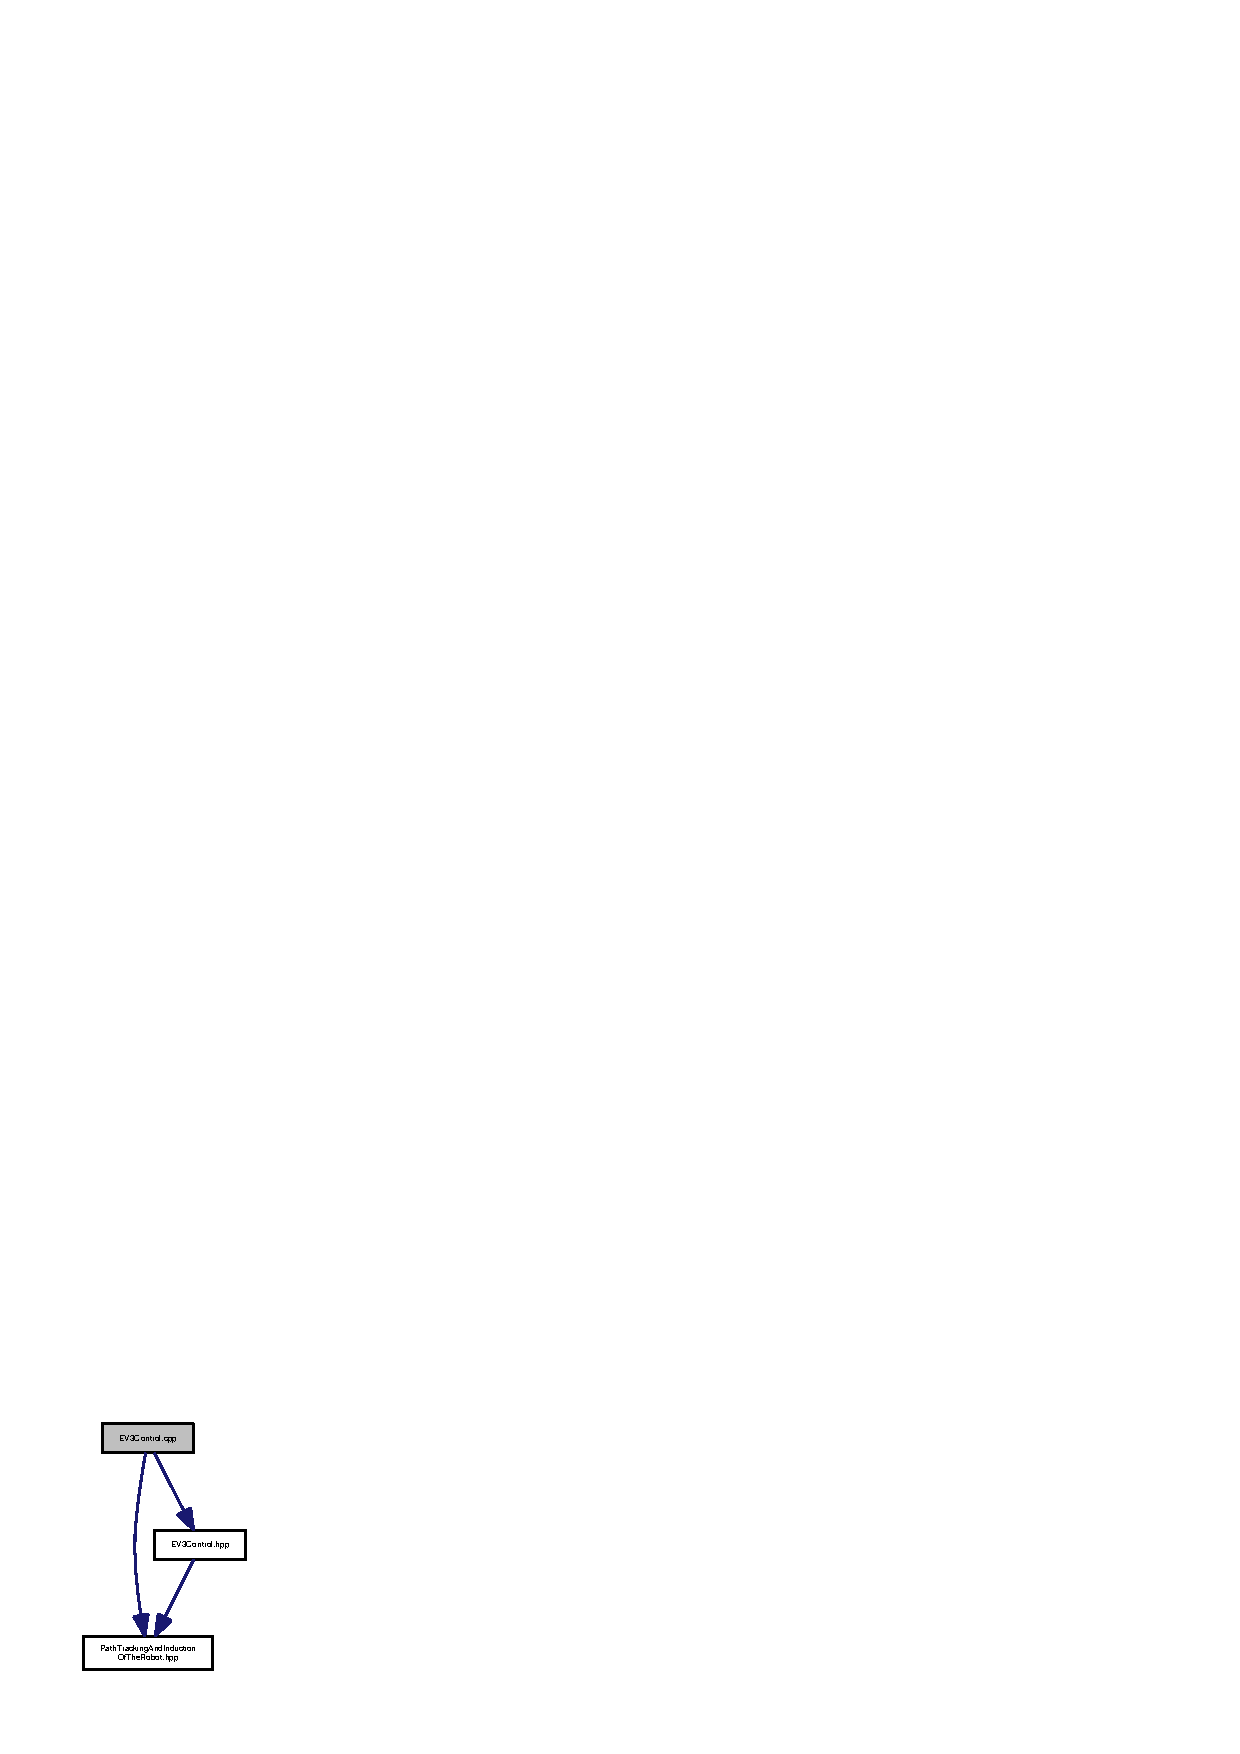
\includegraphics[width=122pt]{_e_v3_control_8cpp__incl}
\end{center}
\end{figure}

\section{E\-V3\-Control.\-hpp ファイル}
\label{_e_v3_control_8hpp}\index{E\-V3\-Control.\-hpp@{E\-V3\-Control.\-hpp}}
{\ttfamily \#include \char`\"{}Path\-Tracking\-And\-Induction\-Of\-The\-Robot.\-hpp\char`\"{}}\\*
E\-V3\-Control.\-hpp の依存先関係図\-:\nopagebreak
\begin{figure}[H]
\begin{center}
\leavevmode
\includegraphics[width=106pt]{_e_v3_control_8hpp__incl}
\end{center}
\end{figure}
被依存関係図\-:\nopagebreak
\begin{figure}[H]
\begin{center}
\leavevmode
\includegraphics[width=138pt]{_e_v3_control_8hpp__dep__incl}
\end{center}
\end{figure}
\subsection*{クラス}
\begin{DoxyCompactItemize}
\item 
class {\bf E\-V3\-Control}
\begin{DoxyCompactList}\small\item\em E\-V3を制御するためのクラス \end{DoxyCompactList}\end{DoxyCompactItemize}

\section{Image\-Processing.\-cpp ファイル}
\label{_image_processing_8cpp}\index{Image\-Processing.\-cpp@{Image\-Processing.\-cpp}}
{\ttfamily \#include \char`\"{}Path\-Tracking\-And\-Induction\-Of\-The\-Robot.\-hpp\char`\"{}}\\*
{\ttfamily \#include \char`\"{}Image\-Processing.\-hpp\char`\"{}}\\*

\section{Image\-Processing.\-hpp ファイル}
\label{_image_processing_8hpp}\index{Image\-Processing.\-hpp@{Image\-Processing.\-hpp}}
{\ttfamily \#include \char`\"{}Path\-Tracking\-And\-Induction\-Of\-The\-Robot.\-hpp\char`\"{}}\\*
\subsection*{クラス}
\begin{DoxyCompactItemize}
\item 
class {\bf Image\-Processing}
\begin{DoxyCompactList}\small\item\em 画像処理用のクラス \end{DoxyCompactList}\end{DoxyCompactItemize}

\section{Kinect.\-cpp ファイル}
\label{_kinect_8cpp}\index{Kinect.\-cpp@{Kinect.\-cpp}}
{\ttfamily \#include \char`\"{}Path\-Tracking\-And\-Induction\-Of\-The\-Robot.\-hpp\char`\"{}}\\*
{\ttfamily \#include \char`\"{}Kinect.\-hpp\char`\"{}}\\*

\section{Kinect.\-hpp ファイル}
\label{_kinect_8hpp}\index{Kinect.\-hpp@{Kinect.\-hpp}}
{\ttfamily \#include \char`\"{}Path\-Tracking\-And\-Induction\-Of\-The\-Robot.\-hpp\char`\"{}}\\*
\subsection*{クラス}
\begin{DoxyCompactItemize}
\item 
class {\bf Kinect}
\begin{DoxyCompactList}\small\item\em Kinect操作用のクラス \end{DoxyCompactList}\end{DoxyCompactItemize}
\subsection*{マクロ定義}
\begin{DoxyCompactItemize}
\item 
\#define {\bf E\-R\-R\-O\-R\-\_\-\-C\-H\-E\-C\-K}(ret)
\begin{DoxyCompactList}\small\item\em エラーチェック \end{DoxyCompactList}\end{DoxyCompactItemize}
\subsection*{変数}
\begin{DoxyCompactItemize}
\item 
const N\-U\-I\-\_\-\-I\-M\-A\-G\-E\-\_\-\-R\-E\-S\-O\-L\-U\-T\-I\-O\-N {\bf C\-A\-M\-E\-R\-A\-\_\-\-R\-E\-S\-O\-L\-U\-T\-I\-O\-N} = N\-U\-I\-\_\-\-I\-M\-A\-G\-E\-\_\-\-R\-E\-S\-O\-L\-U\-T\-I\-O\-N\-\_\-640x480
\end{DoxyCompactItemize}


\subsection{マクロ定義詳解}
\index{Kinect.\-hpp@{Kinect.\-hpp}!E\-R\-R\-O\-R\-\_\-\-C\-H\-E\-C\-K@{E\-R\-R\-O\-R\-\_\-\-C\-H\-E\-C\-K}}
\index{E\-R\-R\-O\-R\-\_\-\-C\-H\-E\-C\-K@{E\-R\-R\-O\-R\-\_\-\-C\-H\-E\-C\-K}!Kinect.hpp@{Kinect.\-hpp}}
\subsubsection[{E\-R\-R\-O\-R\-\_\-\-C\-H\-E\-C\-K}]{\setlength{\rightskip}{0pt plus 5cm}\#define E\-R\-R\-O\-R\-\_\-\-C\-H\-E\-C\-K(
\begin{DoxyParamCaption}
\item[{}]{ret}
\end{DoxyParamCaption}
)}\label{_kinect_8hpp_a60155ea06e80f9ce19fbf58d043f3287}
{\bfseries 値\-:}
\begin{DoxyCode}
\textcolor{keywordflow}{if} (ret != S\_OK)\{ \(\backslash\)
stringstream ss; \(\backslash\)
ss << \textcolor{stringliteral}{"faild"} #ret \textcolor{stringliteral}{" "} << hex << ret << endl; \(\backslash\)
throw runtime\_error(ss.str().c\_str()); \(\backslash\)
\}
\end{DoxyCode}


エラーチェック 



 Kinect.\-hpp の 17 行目に定義があります。



参照元 Kinect\-::create\-Instance(), Kinect\-::draw\-R\-G\-B\-Image(), Kinect\-::get\-Point\-Cloud(), Kinect\-::initialize().



\subsection{変数詳解}
\index{Kinect.\-hpp@{Kinect.\-hpp}!C\-A\-M\-E\-R\-A\-\_\-\-R\-E\-S\-O\-L\-U\-T\-I\-O\-N@{C\-A\-M\-E\-R\-A\-\_\-\-R\-E\-S\-O\-L\-U\-T\-I\-O\-N}}
\index{C\-A\-M\-E\-R\-A\-\_\-\-R\-E\-S\-O\-L\-U\-T\-I\-O\-N@{C\-A\-M\-E\-R\-A\-\_\-\-R\-E\-S\-O\-L\-U\-T\-I\-O\-N}!Kinect.hpp@{Kinect.\-hpp}}
\subsubsection[{C\-A\-M\-E\-R\-A\-\_\-\-R\-E\-S\-O\-L\-U\-T\-I\-O\-N}]{\setlength{\rightskip}{0pt plus 5cm}const N\-U\-I\-\_\-\-I\-M\-A\-G\-E\-\_\-\-R\-E\-S\-O\-L\-U\-T\-I\-O\-N C\-A\-M\-E\-R\-A\-\_\-\-R\-E\-S\-O\-L\-U\-T\-I\-O\-N = N\-U\-I\-\_\-\-I\-M\-A\-G\-E\-\_\-\-R\-E\-S\-O\-L\-U\-T\-I\-O\-N\-\_\-640x480}\label{_kinect_8hpp_ac0e005483bfce51f732e38048c0b1898}
Kinectの解像度の設定 

 Kinect.\-hpp の 25 行目に定義があります。



参照元 Kinect\-::get\-Point\-Cloud(), Kinect\-::initialize().


\section{Least\-Square\-Method.\-cpp ファイル}
\label{_least_square_method_8cpp}\index{Least\-Square\-Method.\-cpp@{Least\-Square\-Method.\-cpp}}
{\ttfamily \#include \char`\"{}Path\-Tracking\-And\-Induction\-Of\-The\-Robot.\-hpp\char`\"{}}\\*
{\ttfamily \#include \char`\"{}Least\-Square\-Method.\-hpp\char`\"{}}\\*
Least\-Square\-Method.\-cpp の依存先関係図\-:\nopagebreak
\begin{figure}[H]
\begin{center}
\leavevmode
\includegraphics[width=134pt]{_least_square_method_8cpp__incl}
\end{center}
\end{figure}

\section{Least\-Square\-Method.\-hpp ファイル}
\label{_least_square_method_8hpp}\index{Least\-Square\-Method.\-hpp@{Least\-Square\-Method.\-hpp}}
{\ttfamily \#include \char`\"{}Path\-Tracking\-And\-Induction\-Of\-The\-Robot.\-hpp\char`\"{}}\\*
Least\-Square\-Method.\-hpp の依存先関係図\-:\nopagebreak
\begin{figure}[H]
\begin{center}
\leavevmode
\includegraphics[width=106pt]{_least_square_method_8hpp__incl}
\end{center}
\end{figure}
被依存関係図\-:\nopagebreak
\begin{figure}[H]
\begin{center}
\leavevmode
\includegraphics[width=154pt]{_least_square_method_8hpp__dep__incl}
\end{center}
\end{figure}
\subsection*{クラス}
\begin{DoxyCompactItemize}
\item 
class {\bf Least\-Square\-Method}
\begin{DoxyCompactList}\small\item\em 最小二乗法を行うクラス \end{DoxyCompactList}\end{DoxyCompactItemize}

\section{main.\-cpp ファイル}
\label{main_8cpp}\index{main.\-cpp@{main.\-cpp}}
{\ttfamily \#include \char`\"{}Path\-Tracking\-And\-Induction\-Of\-The\-Robot.\-hpp\char`\"{}}\\*
{\ttfamily \#include \char`\"{}Kinect.\-hpp\char`\"{}}\\*
{\ttfamily \#include \char`\"{}Image\-Processing.\-hpp\char`\"{}}\\*
{\ttfamily \#include \char`\"{}Drawing.\-hpp\char`\"{}}\\*
{\ttfamily \#include \char`\"{}System.\-hpp\char`\"{}}\\*
{\ttfamily \#include \char`\"{}Least\-Square\-Method.\-hpp\char`\"{}}\\*
{\ttfamily \#include \char`\"{}Point\-Cloud\-Library.\-hpp\char`\"{}}\\*
{\ttfamily \#include \char`\"{}E\-V3\-Control.\-hpp\char`\"{}}\\*
\subsection*{関数}
\begin{DoxyCompactItemize}
\item 
void {\bf on\-Mouse} (int event, int x, int y, int flags, void $\ast$param)
\begin{DoxyCompactList}\small\item\em マウス操作 \end{DoxyCompactList}\item 
int {\bf main} ()
\begin{DoxyCompactList}\small\item\em 関数main() \end{DoxyCompactList}\end{DoxyCompactItemize}
\subsection*{変数}
\begin{DoxyCompactItemize}
\item 
Mat {\bf image}
\begin{DoxyCompactList}\small\item\em R\-G\-B画像格納用の変数 \end{DoxyCompactList}\item 
char {\bf directory\-Name} [{\bf N\-O\-C}]
\begin{DoxyCompactList}\small\item\em フォルダ名 \end{DoxyCompactList}\item 
bool {\bf select\-Object} = false
\begin{DoxyCompactList}\small\item\em オブジェクト選択 \end{DoxyCompactList}\item 
int {\bf track\-Object} = 0
\begin{DoxyCompactList}\small\item\em 追跡するオブジェクト \end{DoxyCompactList}\item 
Point {\bf origin}
\begin{DoxyCompactList}\small\item\em オリジナルの座標 \end{DoxyCompactList}\item 
Rect {\bf selection}
\begin{DoxyCompactList}\small\item\em 選択 \end{DoxyCompactList}\item 
int {\bf save\-\_\-count} = 0
\end{DoxyCompactItemize}


\subsection{関数詳解}
\index{main.\-cpp@{main.\-cpp}!main@{main}}
\index{main@{main}!main.cpp@{main.\-cpp}}
\subsubsection[{main}]{\setlength{\rightskip}{0pt plus 5cm}int main (
\begin{DoxyParamCaption}
{}
\end{DoxyParamCaption}
)}\label{main_8cpp_ae66f6b31b5ad750f1fe042a706a4e3d4}


関数main() 


\begin{DoxyParams}{引数}
{\em なし} & \\
\hline
\end{DoxyParams}
\begin{DoxyReturn}{戻り値}
なし 
\end{DoxyReturn}
$<$システム的なメソッドをまとめているクラス

$<$drawingクラスのインスタンスを生成

$<$最小二乗法を行うクラスのインスタンスを生成(c49)

$<$E\-V3を制御する用のクラスを作成(c80)

$<$E\-V3の軌道を保存するためのフラグ(c82)

$<$背景画像(c75)

pointcloudlibrary.\-viewer-\/$>$was\-Stopped() \&\& 

 main.\-cpp の 39 行目に定義があります。



参照先 System\-::alternatives(), Least\-Square\-Method\-::calc\-Yaw\-Roll\-Pitch(), Point\-Cloud\-Library\-::centroid, System\-::check\-Directory(), Image\-Processing\-::closing\-\_\-times, System\-::countdown\-Timer(), Point\-Cloud\-Library\-::downsampling\-\_\-flag, Point\-Cloud\-Library\-::down\-Sampling\-Using\-Voxel\-Grid\-Filter(), Kinect\-::draw\-R\-G\-B\-Image(), System\-::end\-Message(), System\-::end\-Timer(), E\-V3\-Control\-::ev3\-\_\-6dof, Point\-Cloud\-Library\-::extractplane\-\_\-flag, Point\-Cloud\-Library\-::flag\-Checker(), Image\-Processing\-::get\-Background\-Substraction\-Bin\-Image(), Point\-Cloud\-Library\-::get\-Centroid\-Coordinate3d(), Least\-Square\-Method\-::get\-Coefficient(), Point\-Cloud\-Library\-::get\-Extract\-Plane\-And\-Clustering(), System\-::get\-Frame\-Rate(), Kinect\-::get\-Point\-Cloud(), System\-::get\-Process\-Timein\-Miliseconds(), Image\-Processing\-::get\-Undistortion\-Image(), Drawing\-::gnuplot\-Script\-E\-V3\-Route(), Drawing\-::gnuplot\-Script\-E\-V3\-Unit(), image, Kinect\-::initialize(), Point\-Cloud\-Library\-::initialize\-P\-C\-L\-Visualizer(), Kinect\-::key, Image\-Processing\-::load\-Internal\-Camera\-Parameter(), System\-::make\-Directory(), Point\-Cloud\-Library\-::mls\-\_\-flag, Image\-Processing\-::neighborhood, Point\-Cloud\-Library\-::passthrough\-\_\-flag, Point\-Cloud\-Library\-::pass\-Through\-Filter(), System\-::remove\-Directory(), Point\-Cloud\-Library\-::remove\-Outlier(), save\-\_\-count, System\-::save\-\_\-flag, System\-::save\-Data\-Continuously(), System\-::save\-Data\-Every\-Enter\-Key(), E\-V3\-Control\-::set6\-Do\-F\-E\-V3(), Image\-Processing\-::show\-Image(), Point\-Cloud\-Library\-::smoothing\-Using\-Moving\-Least\-Square(), System\-::start\-Message(), System\-::start\-Timer(), Point\-Cloud\-Library\-::statisticaloutlierremoval\-\_\-flag, Kinect\-::stream\-Event, Image\-Processing\-::th, Point\-Cloud\-Library\-::visualizer (計49項目).


\begin{DoxyCode}
40 \{
41     RETRY: \textcolor{comment}{//goto文.再計測をやり直す場合}
42     \textcolor{comment}{//インスタンスの生成}
43     Kinect kinect; \textcolor{comment}{//Kinectクラスのインスタンスを生成}
44     System sys; 
45     ImageProcessing imgproc; \textcolor{comment}{//Imageprocessingクラスのインスタンスを生成}
46     Drawing draw; 
47     LeastSquareMethod lsm; 
48     PointCloudLibrary pointcloudlibrary(\textcolor{comment}{/*false*/}\textcolor{keyword}{true}, \textcolor{comment}{/*false*/}\textcolor{keyword}{true}, \textcolor{comment}{/*false*/}\textcolor{keyword}{true}, \textcolor{keyword}{false}, \textcolor{keyword}{false}\textcolor{comment}{/*true*/});
       \textcolor{comment}{//PointCloudLibraryクラスのインスタンスを生成(c57)}
49     EV3Control ev3control; 
50 
51     \textcolor{comment}{//変数の宣言}
52     \textcolor{keywordtype}{bool} saveev3route\_flag = \textcolor{keyword}{false}; 
53 
54     \textcolor{comment}{//画像関係の変数}
55     Mat flip\_image; \textcolor{comment}{//確認用に反転した画像}
56     Mat current\_image; \textcolor{comment}{//現在のフレームの画像(c75)}
57     Mat bin\_image; \textcolor{comment}{//背景差分によって得られた二値画像(c75)}
58     Mat background\_image; 
59     Mat background\_gray\_image;
60 
61     \textcolor{comment}{//ポイントクラウド関係の変数(c57)}
62     pcl::PointCloud<pcl::PointXYZRGB>::Ptr cloud; \textcolor{comment}{//処理を受け取る点群}
63 
64     \textcolor{comment}{//EV3ユニットの平面の係数(c78)}
65     Eigen::Vector3f coefficient\_plane; \textcolor{comment}{//平面の係数}
66     AttitudeAngle3d attitude\_angle; \textcolor{comment}{//姿勢角(c78)}
67 
68     \textcolor{comment}{//CloudVisualizermの初期設定(c83)}
69 
70 
71     \textcolor{comment}{//メインの処理}
72     \textcolor{keywordflow}{try}\{
73         sys.startMessage(); \textcolor{comment}{//プログラム開始時のメッセージを表示}
74         \textcolor{comment}{//初期設定(利用する場合はコメントを外す)}
75         \textcolor{comment}{//pointcloudlibrary.loadPLY("EV3COLOR.ply"); //.plyファイルの読み込み.動作しない}
76         \textcolor{comment}{//VideoWriter writer; //動画保存用 }
77 
78         \textcolor{comment}{//ウインドウ名とファイル名の定義}
79         \textcolor{keyword}{const} \textcolor{keywordtype}{string} main\_windowname = \textcolor{stringliteral}{"Current Image"}; \textcolor{comment}{//メインウインドウの名前をつけておく.(c31)}
80         \textcolor{keyword}{const} \textcolor{keywordtype}{string} backgroundimage\_windowname = \textcolor{stringliteral}{"Background Image"}; \textcolor{comment}{//背景画像を表示するためのウインドウ名}
81         \textcolor{keyword}{const} \textcolor{keywordtype}{string} maskbinimage\_windowname = \textcolor{stringliteral}{"Mask Image"}; \textcolor{comment}{//マスク画像を表示するためのウインドウ名}
82         \textcolor{comment}{//const string outputVideoName = "video.avi"; //計測中の動画ファイル名(c39)}
83         \textcolor{keyword}{const} \textcolor{keywordtype}{string} cameraparameter\_name = \textcolor{stringliteral}{"sourcedata/cameraParam.xml"}; \textcolor{comment}{//
      xmlファイル名の定義.カメラキャリブレーションによって得られたファイル名(c54)}
84         \textcolor{keyword}{const} \textcolor{keywordtype}{char}* basedirectory\_name = \textcolor{stringliteral}{"data"}; \textcolor{comment}{//データ保存先のディレクトリ名}
85         \textcolor{keyword}{const} \textcolor{keywordtype}{string} cloudviewer\_windowname = \textcolor{stringliteral}{"Cloud Viewer"}; \textcolor{comment}{//クラウドビューアーの名前の定義(c81)}
86         \textcolor{keyword}{const} \textcolor{keywordtype}{string} pclvisualizer\_windowname = \textcolor{stringliteral}{"3D Viewer"};
87         \textcolor{keyword}{const} \textcolor{keywordtype}{string} param\_windowname = \textcolor{stringliteral}{"OpenCV Parameter Setting Window"}; \textcolor{comment}{//パラメータ調整用のウインドウ(c82)}
88 
89         kinect.initialize(); \textcolor{comment}{//Kinectの初期化}
90         sys.checkDirectory(basedirectory\_name); \textcolor{comment}{//base\_directoryが存在するか確認し,存在しなければ作成(c81)}
91         sys.makeDirectory(); \textcolor{comment}{//起動時刻をフォルダ名にしてフォルダを作成}
92         
93         \textcolor{comment}{//動画を保存するために利用する(c40)}
94         \textcolor{comment}{//writer = sys.outputVideo(&outputVideoName); //動画を保存したいときはコメントをはずす.while文内のwriter << imageのコメントも}
95 
96         imgproc.loadInternalCameraParameter(cameraparameter\_name); \textcolor{comment}{//キャリブレーションを行うためのパラメータを取得(c79)}
97 
98         \textcolor{comment}{//背景用に一度撮影(c75)}
99         cout << \textcolor{stringliteral}{"Take a Background Image in "} << endl;
100         sys.countdownTimer(3);
101         system(\textcolor{stringliteral}{"cls"});
102         DWORD ret = ::WaitForSingleObject(kinect.streamEvent, INFINITE); \textcolor{comment}{//フレーム更新をイベントとして待つ}
103         ::ResetEvent(kinect.streamEvent); \textcolor{comment}{//イベントが発生したら次のイベントに備えてリセット}
104         \textcolor{comment}{//Kinectから画像を取得し,背景画像とする}
105         PlaySound(TEXT(\textcolor{stringliteral}{"sourcedata/shutter.wav"}), NULL, (SND\_ASYNC | SND\_FILENAME)); \textcolor{comment}{//音声ファイルを再生}
106         background\_image = kinect.drawRGBImage(image); \textcolor{comment}{//RGBカメラの処理}
107         background\_image = imgproc.getUndistortionImage(background\_image); \textcolor{comment}{//キャリブレーション後の画像を今の背景画像とする}
108         imgproc.showImage(backgroundimage\_windowname, background\_image); \textcolor{comment}{//背景画像を表示する}
109         cvtColor(background\_image, background\_gray\_image, CV\_BGR2GRAY); \textcolor{comment}{//グレースケールに変換}
110         
111         Sleep(1000);
112 
113         \textcolor{comment}{//プログラム開始の通知}
114         cout << \textcolor{stringliteral}{"Process will Start in "} << endl;
115         sys.countdownTimer(2); 
116         PlaySound(TEXT(\textcolor{stringliteral}{"sourcedata/shutter.wav"}), NULL, (SND\_ASYNC | SND\_FILENAME)); \textcolor{comment}{//音声ファイルを再生}
117         system(\textcolor{stringliteral}{"cls"}); \textcolor{comment}{//コンソール内の表示をリセット(c64)}
118 
119         \textcolor{comment}{//pointcloudlibrary.initializePointCloudViewer(cloudviewer\_windowname); //クラウドビューアーの初期化}
120         pointcloudlibrary.initializePCLVisualizer(pclvisualizer\_windowname);
121 
122         \textcolor{comment}{//namedWindow("閾値", 1);}
123         \textcolor{keywordflow}{while} (!pointcloudlibrary.visualizer->wasStopped() && kinect.key != \textcolor{charliteral}{'q'} && !GetAsyncKeyState(\textcolor{charliteral}{'Q'}))\{
       \textcolor{comment}{//(c3).メインループ.1フレームごとの処理を繰り返し行う.(c63)CloudViewerが終了処理('q'キーを入力)したらプログラムが終了する}
124             \textcolor{comment}{//タイマー開始(c65)}
125             sys.startTimer();
126 
127             \textcolor{comment}{//setMouseCallback(mainwindow\_name, onMouse, 0); //(c25).マウスコールバック関数をセット(c31)}
128 
129             DWORD ret = ::WaitForSingleObject(kinect.streamEvent, INFINITE); \textcolor{comment}{//フレーム更新をイベントとして待つ}
130             ::ResetEvent(kinect.streamEvent); \textcolor{comment}{//イベントが発生したら次のイベントに備えてリセット}
131 
132             \textcolor{comment}{//Kinectから画像を取得し,画像処理を行う}
133             current\_image = kinect.drawRGBImage(image); \textcolor{comment}{//RGBカメラの処理}
134             current\_image = imgproc.getUndistortionImage(current\_image); \textcolor{comment}{//
      Kinectのキャリブレーションを行い,キャリブレーション結果を適用する(c71)}
135             imgproc.showImage(main\_windowname, current\_image);
136             \textcolor{comment}{//flip(current\_image, flip\_image, 1);}
137             \textcolor{comment}{//imgproc.showImage("Original - Flip", flip\_image); //Kinectから取得した画像を表示}
138             
139             \textcolor{comment}{//タイヤも含めて前面の点群を取得する}
140             namedWindow(param\_windowname, CV\_WINDOW\_KEEPRATIO);
141             createTrackbar(\textcolor{stringliteral}{"Threshold(0-255)"}, param\_windowname, &imgproc.th, 255);
142             createTrackbar(\textcolor{stringliteral}{"Neighborhood Level(0-10)"}, param\_windowname, &imgproc.
      neighborhood, 10);
143             createTrackbar(\textcolor{stringliteral}{"Closing Times Level(0-10)"}, param\_windowname, &imgproc.
      closing_times, 10);
144             bin\_image = imgproc.getBackgroundSubstractionBinImage(current\_image, background\_gray\_image\textcolor{comment}{/*,
       imgproc.th, imgproc.med, imgproc.cnt*/});
145             \textcolor{comment}{//ユニット部だけ切り取る(c77)}
146             \textcolor{comment}{//bin\_image = imgproc.getUnitMask(bin\_image);}
147             imgproc.showImage(maskbinimage\_windowname, bin\_image); \textcolor{comment}{//確認用に切り取った画像を表示する}
148             
149             \textcolor{comment}{//ポイントクラウドの取得(c57)}
150             cloud = kinect.getPointCloud(bin\_image); \textcolor{comment}{//ポイントクラウドの取得(c57).切り取った画像をもとにする}
151             pointcloudlibrary.flagChecker(); \textcolor{comment}{//各点群処理のフラグをチェックするメソッド(c64)}
152             cout << \textcolor{stringliteral}{"
      =========================================================================================="} << endl;
153             cout << \textcolor{stringliteral}{"Original PointCloud Size\(\backslash\)t=>\(\backslash\)t"} << cloud->size() << endl;
154 
155             \textcolor{comment}{//PCLの処理}
156             \textcolor{keywordflow}{if} (pointcloudlibrary.passthrough\_flag == \textcolor{keyword}{true})\{  \textcolor{comment}{//外れ値除去(c59)}
157                 cloud = pointcloudlibrary.passThroughFilter(cloud, \textcolor{stringliteral}{"z"}, 400, 30000); \textcolor{comment}{//
      Kinectから取得した外れ値を除去(c60).与えた軸の中で自分が取得したい範囲の下限と上限を与えることでそれ以外を省く(c81)}
158                 \textcolor{comment}{//cloud = pointcloudlibrary.radiusOutlierRemoval(cloud); //半径を指定して外れ値を除去(c60)}
159             \}
160 
161             \textcolor{keywordflow}{if} (pointcloudlibrary.downsampling\_flag == \textcolor{keyword}{true})\{   \textcolor{comment}{//ダウンサンプリング処理(c59)}
162                 \textcolor{comment}{//cloud = pointcloudlibrary.downSamplingUsingVoxelGridFilter(pointcloudlibrary.cloud, 2.0f,
       2.0f, 2.0f); //Default=all 0.003}
163                 cloud = pointcloudlibrary.downSamplingUsingVoxelGridFilter(cloud, 2.5f, 2.5f, 2.5f); \textcolor{comment}{//
      Default=all 0.003}
164                 \textcolor{comment}{//pointcloudlibrary.cloud =
       pointcloudlibrary.downSamplingUsingVoxelGridFilter(pointcloudlibrary.cloud, 0.001, 0.001, 0.001); //Default=all 0.003}
165             \}
166 
167             \textcolor{keywordflow}{if} (pointcloudlibrary.statisticaloutlierremoval\_flag == \textcolor{keyword}{true})\{
168                 cloud = pointcloudlibrary.removeOutlier(cloud); \textcolor{comment}{//統計的な外れ値除去(c60)}
169             \}
170 
171             \textcolor{keywordflow}{if} (pointcloudlibrary.downsampling\_flag == \textcolor{keyword}{true} && pointcloudlibrary.mls\_flag == \textcolor{keyword}{true})\{  \textcolor{comment}{//
      スムージング処理(c60)}
172                 cloud = pointcloudlibrary.smoothingUsingMovingLeastSquare(cloud, \textcolor{keyword}{true}, \textcolor{keyword}{true}, 2.5); \textcolor{comment}{//0.002
       < radius < ◯.小さいほど除去される}
173 
174             \}
175             \textcolor{keywordflow}{else} \textcolor{keywordflow}{if} (pointcloudlibrary.downsampling\_flag == \textcolor{keyword}{false} && pointcloudlibrary.mls\_flag == \textcolor{keyword}{true})\{
176                 cout << \textcolor{stringliteral}{"MLSを有効にするためには,ダウンサンプリングを有効にしてください"} << endl;
177             \}
178 
179             \textcolor{keywordflow}{if} (pointcloudlibrary.extractplane\_flag == \textcolor{keyword}{true})\{   \textcolor{comment}{//平面検出とクラスタリング(c61)}
180                 cloud = pointcloudlibrary.getExtractPlaneAndClustering(cloud, \textcolor{keyword}{true}, 100, 5, \textcolor{keyword}{false}, \textcolor{keyword}{true}, 0.
      02, \textcolor{comment}{/*350*/}150, \textcolor{comment}{/*25000*/}\textcolor{comment}{/*20000*/}200000); \textcolor{comment}{//Default=0.03(前処理なしの場合)}
181             \}
182 
183             pointcloudlibrary.centroid = pointcloudlibrary.getCentroidCoordinate3d(cloud); \textcolor{comment}{//重心座標の計算}
184             
185             
186             coefficient\_plane = lsm.getCoefficient(cloud); \textcolor{comment}{//最小二乗法を行い平面の係数[a b c]'を取得する(c78)}
187             attitude\_angle = lsm.calcYawRollPitch(coefficient\_plane); \textcolor{comment}{//姿勢角を取得(c78)}
188             \textcolor{comment}{//cout << "[Yaw, Roll, Pitch]" << attitude\_angle.yaw << " , " << attitude\_angle.roll << " , "
       << attitude\_angle.pitch << endl;}
189             
190             ev3control.set6DoFEV3(cloud, pointcloudlibrary.centroid, attitude\_angle); \textcolor{comment}{//6DoFをまとめる}
191             
192             \textcolor{comment}{//平均座標に球を描画する(c83)}
193             pcl::PointXYZ sphere;
194             sphere.x = pointcloudlibrary.centroid.x; \textcolor{comment}{//平均座標のx座標}
195             sphere.y = pointcloudlibrary.centroid.y; \textcolor{comment}{//平均座標のy座標}
196             sphere.z = pointcloudlibrary.centroid.z; \textcolor{comment}{//平均座標のz座標}
197             pointcloudlibrary.visualizer->addSphere(sphere, 10, 0.5, 0.0, 0.0, \textcolor{stringliteral}{"sphere"}); \textcolor{comment}{//平均座標に球を描画}
198 
199             \textcolor{comment}{//Kinectから取得した点群を描画}
200             pointcloudlibrary.visualizer->addPointCloud(cloud, \textcolor{stringliteral}{"show cloud"}); \textcolor{comment}{//点群を描画}
201             \textcolor{comment}{//visualizer->updatePointCloud<pcl::PointXYZRGB>(cloud, "show cloud");}
202             cout << \textcolor{stringliteral}{"
      =========================================================================================="} << endl;
203 
204             \textcolor{comment}{//pointcloudlibrary.viewer->showCloud(cloud); //処理後の点群を表示}
205             pointcloudlibrary.visualizer->spinOnce(); \textcolor{comment}{//PCLVisualizerを描画}
206             \textcolor{comment}{//終了のためのキー入力チェック兼表示のためのウェイトタイム}
207             kinect.key = waitKey(1); \textcolor{comment}{//OpenCVのウインドウを表示し続ける}
208 
209             \textcolor{comment}{//PCLのフレームレートを計算する用(c61)}
210             sys.endTimer(); \textcolor{comment}{//タイマーを終了(c65)}
211             cout << sys.getProcessTimeinMiliseconds() << \textcolor{stringliteral}{"[ms], "} << sys.
      getFrameRate() << \textcolor{stringliteral}{" fps"} << \textcolor{stringliteral}{"\(\backslash\)n"} << endl;
212 
213             \textcolor{comment}{//キーが入力されていれば以下を実行する.GetAsyncKeyStateを利用することで}
214             \textcolor{keywordflow}{if} (GetAsyncKeyState(\textcolor{charliteral}{'R'}))\{
215                 system(\textcolor{stringliteral}{"cls"});
216                 destroyAllWindows(); \textcolor{comment}{//PCLまたは,OpenCV画面上で'q'キーが入力されたらOpenCVのウインドウを閉じて処理を終了(c66)}
217                 \textcolor{comment}{//pointcloudlibrary.viewer->~CloudViewer(); //クラウドビューアーの削除}
218                 sys.removeDirectory(); \textcolor{comment}{//再計測を行う場合は,現在のデータは必要ないため削除}
219                 cout << \textcolor{stringliteral}{"Data Removed."} << endl;
220                 save_count = 0;
221                 system(\textcolor{stringliteral}{"cls"}); \textcolor{comment}{//cmdをクリア}
222                 cout << \textcolor{stringliteral}{"RETRY"} << endl;
223                 \textcolor{keywordflow}{goto} RETRY;
224             \}
225             \textcolor{keywordflow}{else} \textcolor{keywordflow}{if} (GetAsyncKeyState(\textcolor{charliteral}{'P'}))\{ \textcolor{comment}{//その時点のデータを保存する.複数回データを計測する際はプログラムを起動しなおす手間が省ける}
226                 cout << \textcolor{stringliteral}{"Save the Current Data."} << endl;
227                 sys.saveDataEveryEnterKey(current\_image,bin\_image,ev3control.
      ev3_6dof, cloud);
228                 draw.gnuplotScriptEV3Unit(coefficient\_plane); \textcolor{comment}{//gnuplot用のスクリプト}
229                 sys.save_flag = \textcolor{keyword}{true}; \textcolor{comment}{//6DoF情報を出力するフラグをオンにする(c82)}
230                 save_count++;
231             \}
232             \textcolor{keywordflow}{else} \textcolor{keywordflow}{if} (GetAsyncKeyState(\textcolor{charliteral}{'L'}))\{ \textcolor{comment}{//'l'が入力されたら.EV3軌道が欲しい時に入力する}
233                 saveev3route\_flag = \textcolor{keyword}{true}; \textcolor{comment}{//フラグをtrueにする}
234             \}
235 
236             \textcolor{comment}{//'l'キーが入力されていれば,平均座標の軌道を追跡し続ける(c82)}
237             \textcolor{keywordflow}{if} (saveev3route\_flag == \textcolor{keyword}{true})\{ \textcolor{comment}{//フラグがtrueであれば,平均座標の軌道を保存する(c82)}
238                 sys.saveDataContinuously(ev3control.ev3_6dof);
239             \}
240 
241             \textcolor{comment}{//PCLVisualizerに描画した点群を削除する}
242             pointcloudlibrary.visualizer->removePointCloud(\textcolor{stringliteral}{"show cloud"});
243             pointcloudlibrary.visualizer->removeShape(\textcolor{stringliteral}{"sphere"});
244 
245             system(\textcolor{stringliteral}{"cls"}); \textcolor{comment}{//コンソール内の表示をリセット(c64)}
246         \}
247 
248         \textcolor{comment}{//計測が終了したところ(PCL上, OpenCVウインドウ上, コンソール上で'q'が押されてたとき)}
249         destroyAllWindows(); \textcolor{comment}{//PCLまたは,OpenCV画面上で'q'キーが入力されたらOpenCVのウインドウを閉じて処理を終了(c66)}
250         \textcolor{comment}{//pointcloudlibrary.viewer->~CloudViewer(); //クラウドビューアーの削除}
251         pointcloudlibrary.visualizer->~PCLVisualizer(); \textcolor{comment}{//PCLVisualizerの削除}
252         \textcolor{keywordflow}{if} (saveev3route\_flag == \textcolor{keyword}{true})\{ \textcolor{comment}{//一度でもデータを保存していれば,どちらかのフラグはtrueになる}
253             draw.gnuplotScriptEV3Route(); \textcolor{comment}{//軌道をプロットするスクリプトを保存する}
254         \}
255 
256         \textcolor{comment}{//データを保存するかの確認}
257         \textcolor{keywordflow}{if} (saveev3route\_flag == \textcolor{keyword}{true} || sys.save_flag == \textcolor{keyword}{true})\{ \textcolor{comment}{//
      データを保存するフラグがtrue(=データが保存されている)なら保存するかどうか確認する}
258             cout << \textcolor{stringliteral}{"Save Data?"} << endl;
259             \textcolor{keywordtype}{int} checkNum = sys.alternatives(); \textcolor{comment}{//'1'なら保存,'0'なら削除}
260             \textcolor{keywordflow}{if} (checkNum == 1)\{
261                 sys.endMessage(checkNum);
262             \}
263         \}
264         \textcolor{keywordflow}{else}\{
265             sys.removeDirectory(); \textcolor{comment}{//ディレクトリの削除}
266             sys.endMessage();
267         \}
268     \}
269     \textcolor{keywordflow}{catch} (exception& ex)\{ \textcolor{comment}{//例外処理}
270         cout << ex.what() << endl;
271         destroyAllWindows(); \textcolor{comment}{//OpenCVで作成したウインドウを全て削除する(c35)}
272         \textcolor{comment}{//pointcloudlibrary.viewer->~CloudViewer(); //クラウドビューアーの削除}
273         pointcloudlibrary.visualizer->~PCLVisualizer(); \textcolor{comment}{//PCLVisualizerの削除}
274         \textcolor{comment}{//異常終了した時はデータを保存する必要がないので削除}
275         sys.removeDirectory();
276         cout << \textcolor{stringliteral}{"Data Removed."} << endl;
277         \textcolor{keywordflow}{return} -1;
278     \}
279     \textcolor{keywordflow}{return} 0;
280 \}\end{DoxyCode}
\index{main.\-cpp@{main.\-cpp}!on\-Mouse@{on\-Mouse}}
\index{on\-Mouse@{on\-Mouse}!main.cpp@{main.\-cpp}}
\subsubsection[{on\-Mouse}]{\setlength{\rightskip}{0pt plus 5cm}void on\-Mouse (
\begin{DoxyParamCaption}
\item[{int}]{event, }
\item[{int}]{x, }
\item[{int}]{y, }
\item[{int}]{flags, }
\item[{void $\ast$}]{param}
\end{DoxyParamCaption}
)}\label{main_8cpp_ab6ccc6c8d80970d4178c943533533860}


マウス操作 



 Mouse.\-cpp の 12 行目に定義があります。


\begin{DoxyCode}
13 \{
14     \textcolor{keywordflow}{if} (selectObject)
15     \{
16         selection.x = MIN(x, origin.x);
17         selection.y = MIN(y, origin.y);
18         selection.width = abs(x - origin.x);
19         selection.height = abs(y - origin.y);
20         selection &= Rect(0, 0, image.cols, image.rows);
21     \}
22 
23     \textcolor{keywordflow}{switch} (event)
24     \{
25     \textcolor{keywordflow}{case} CV\_EVENT\_LBUTTONDOWN:
26         origin = Point(x, y);
27         selection = Rect(x, y, 0, 0);
28         selectObject = \textcolor{keyword}{true};
29         \textcolor{keywordflow}{break};
30     \textcolor{keywordflow}{case} CV\_EVENT\_LBUTTONUP:
31         selectObject = \textcolor{keyword}{false};
32         \textcolor{keywordflow}{if} (selection.width > 0 && selection.height > 0)
33         \{
34             trackObject = -1;
35         \}
36         \textcolor{keywordflow}{break};
37     \}
38 
39     \textcolor{keywordflow}{return};
40 \}\end{DoxyCode}


\subsection{変数詳解}
\index{main.\-cpp@{main.\-cpp}!directory\-Name@{directory\-Name}}
\index{directory\-Name@{directory\-Name}!main.cpp@{main.\-cpp}}
\subsubsection[{directory\-Name}]{\setlength{\rightskip}{0pt plus 5cm}char directory\-Name[{\bf N\-O\-C}]}\label{main_8cpp_abefb498e9a643f68bb3d37c22953ddad}


フォルダ名 



 main.\-cpp の 23 行目に定義があります。



参照元 System\-::end\-Message(), Drawing\-::gnuplot\-Script(), Drawing\-::gnuplot\-Script\-Co\-G(), Drawing\-::gnuplot\-Script\-E\-V3\-Route(), Drawing\-::gnuplot\-Script\-E\-V3\-Unit(), System\-::make\-Directory(), System\-::open\-Directory(), System\-::output\-All\-Data(), System\-::output\-Video(), Drawing\-::plot3\-D(), Drawing\-::plot3\-D\-Real\-Time(), System\-::remove\-Directory(), System\-::save\-Data\-Continuously(), System\-::save\-Data\-Every\-Enter\-Key().

\index{main.\-cpp@{main.\-cpp}!image@{image}}
\index{image@{image}!main.cpp@{main.\-cpp}}
\subsubsection[{image}]{\setlength{\rightskip}{0pt plus 5cm}Mat image}\label{main_8cpp_aabb27b8973575043030df51be47cd24a}


R\-G\-B画像格納用の変数 



 main.\-cpp の 21 行目に定義があります。



参照元 Kinect\-::get\-Point\-Cloud(), main(), on\-Mouse().

\index{main.\-cpp@{main.\-cpp}!origin@{origin}}
\index{origin@{origin}!main.cpp@{main.\-cpp}}
\subsubsection[{origin}]{\setlength{\rightskip}{0pt plus 5cm}Point origin}\label{main_8cpp_a903d0d8820c696aaa1170c50deb3633f}


オリジナルの座標 



 main.\-cpp の 28 行目に定義があります。



参照元 on\-Mouse().

\index{main.\-cpp@{main.\-cpp}!save\-\_\-count@{save\-\_\-count}}
\index{save\-\_\-count@{save\-\_\-count}!main.cpp@{main.\-cpp}}
\subsubsection[{save\-\_\-count}]{\setlength{\rightskip}{0pt plus 5cm}int save\-\_\-count = 0}\label{main_8cpp_aacae5d304dcef5f6bbf0fe5030e50626}


 main.\-cpp の 32 行目に定義があります。



参照元 Drawing\-::gnuplot\-Script\-E\-V3\-Unit(), main(), System\-::save\-Data\-Every\-Enter\-Key().

\index{main.\-cpp@{main.\-cpp}!selection@{selection}}
\index{selection@{selection}!main.cpp@{main.\-cpp}}
\subsubsection[{selection}]{\setlength{\rightskip}{0pt plus 5cm}Rect selection}\label{main_8cpp_a15633c47538e3790df1e008a7f6dbfea}


選択 



 main.\-cpp の 29 行目に定義があります。



参照元 on\-Mouse().

\index{main.\-cpp@{main.\-cpp}!select\-Object@{select\-Object}}
\index{select\-Object@{select\-Object}!main.cpp@{main.\-cpp}}
\subsubsection[{select\-Object}]{\setlength{\rightskip}{0pt plus 5cm}bool select\-Object = false}\label{main_8cpp_a71a276a0dc4ef6aa35740b58f10bcb39}


オブジェクト選択 



 main.\-cpp の 26 行目に定義があります。



参照元 on\-Mouse().

\index{main.\-cpp@{main.\-cpp}!track\-Object@{track\-Object}}
\index{track\-Object@{track\-Object}!main.cpp@{main.\-cpp}}
\subsubsection[{track\-Object}]{\setlength{\rightskip}{0pt plus 5cm}int track\-Object = 0}\label{main_8cpp_a88f176e4e65e22a17093a8cd24003a66}


追跡するオブジェクト 



 main.\-cpp の 27 行目に定義があります。



参照元 on\-Mouse().


\section{Mouse.\-cpp ファイル}
\label{_mouse_8cpp}\index{Mouse.\-cpp@{Mouse.\-cpp}}
{\ttfamily \#include \char`\"{}Path\-Tracking\-And\-Induction\-Of\-The\-Robot.\-hpp\char`\"{}}\\*
Mouse.\-cpp の依存先関係図\-:\nopagebreak
\begin{figure}[H]
\begin{center}
\leavevmode
\includegraphics[width=106pt]{_mouse_8cpp__incl}
\end{center}
\end{figure}
\subsection*{関数}
\begin{DoxyCompactItemize}
\item 
void {\bf on\-Mouse} (int event, int x, int y, int flags, void $\ast$param)
\begin{DoxyCompactList}\small\item\em メソッドon\-Mouse().マウス左クリックで座標を取得するメソッド \end{DoxyCompactList}\end{DoxyCompactItemize}


\subsection{関数詳解}
\index{Mouse.\-cpp@{Mouse.\-cpp}!on\-Mouse@{on\-Mouse}}
\index{on\-Mouse@{on\-Mouse}!Mouse.cpp@{Mouse.\-cpp}}
\subsubsection[{on\-Mouse}]{\setlength{\rightskip}{0pt plus 5cm}void on\-Mouse (
\begin{DoxyParamCaption}
\item[{int}]{event, }
\item[{int}]{x, }
\item[{int}]{y, }
\item[{int}]{flags, }
\item[{void $\ast$}]{param}
\end{DoxyParamCaption}
)}\label{_mouse_8cpp_ab6ccc6c8d80970d4178c943533533860}


メソッドon\-Mouse().マウス左クリックで座標を取得するメソッド 

マウス操作


\begin{DoxyParams}{引数}
{\em event} & int 型.イベント \\
\hline
{\em x} & int型.x座標 \\
\hline
{\em y} & int型.y座標 \\
\hline
{\em flags} & int型.フラグ \\
\hline
{\em param} & void$\ast$型.その他パラメータ \\
\hline
\end{DoxyParams}


 Mouse.\-cpp の 19 行目に定義があります。



参照先 image, origin, selection, select\-Object, track\-Object.


\section{Path\-Tracking\-And\-Induction\-Of\-The\-Robot.\-hpp ファイル}
\label{_path_tracking_and_induction_of_the_robot_8hpp}\index{Path\-Tracking\-And\-Induction\-Of\-The\-Robot.\-hpp@{Path\-Tracking\-And\-Induction\-Of\-The\-Robot.\-hpp}}
\subsection*{クラス}
\begin{DoxyCompactItemize}
\item 
struct {\bf Point3}
\item 
struct {\bf output\-Data}
\item 
struct {\bf Do\-F}
\item 
struct {\bf Attitude\-Angle}
\end{DoxyCompactItemize}
\subsection*{型定義}
\begin{DoxyCompactItemize}
\item 
typedef struct {\bf Point3} {\bf Point3ius}
\item 
typedef struct {\bf output\-Data} {\bf output\-Data}
\item 
typedef struct {\bf Do\-F} {\bf Do\-F6d}
\item 
typedef struct {\bf Attitude\-Angle} {\bf Attitude\-Angle3d}
\end{DoxyCompactItemize}
\subsection*{関数}
\begin{DoxyCompactItemize}
\item 
void {\bf on\-Mouse} (int event, int x, int y, int, void $\ast$)
\begin{DoxyCompactList}\small\item\em マウス操作 \end{DoxyCompactList}\end{DoxyCompactItemize}
\subsection*{変数}
\begin{DoxyCompactItemize}
\item 
Mat {\bf image}
\begin{DoxyCompactList}\small\item\em R\-G\-B画像格納用の変数 \end{DoxyCompactList}\item 
char {\bf directory\-Name} [{\bf N\-O\-C}]
\begin{DoxyCompactList}\small\item\em フォルダ名 \end{DoxyCompactList}\item 
bool {\bf select\-Object}
\begin{DoxyCompactList}\small\item\em オブジェクト選択 \end{DoxyCompactList}\item 
int {\bf track\-Object}
\begin{DoxyCompactList}\small\item\em 追跡するオブジェクト \end{DoxyCompactList}\item 
Point {\bf origin}
\begin{DoxyCompactList}\small\item\em オリジナルの座標 \end{DoxyCompactList}\item 
Rect {\bf selection}
\begin{DoxyCompactList}\small\item\em 選択 \end{DoxyCompactList}\item 
int {\bf save\-\_\-count}
\end{DoxyCompactItemize}


\subsection{型定義詳解}
\index{Path\-Tracking\-And\-Induction\-Of\-The\-Robot.\-hpp@{Path\-Tracking\-And\-Induction\-Of\-The\-Robot.\-hpp}!Attitude\-Angle3d@{Attitude\-Angle3d}}
\index{Attitude\-Angle3d@{Attitude\-Angle3d}!PathTrackingAndInductionOfTheRobot.hpp@{Path\-Tracking\-And\-Induction\-Of\-The\-Robot.\-hpp}}
\subsubsection[{Attitude\-Angle3d}]{\setlength{\rightskip}{0pt plus 5cm}typedef struct {\bf Attitude\-Angle} {\bf Attitude\-Angle3d}}\label{_path_tracking_and_induction_of_the_robot_8hpp_a4860903646946a52474a935518d26b08}
\index{Path\-Tracking\-And\-Induction\-Of\-The\-Robot.\-hpp@{Path\-Tracking\-And\-Induction\-Of\-The\-Robot.\-hpp}!Do\-F6d@{Do\-F6d}}
\index{Do\-F6d@{Do\-F6d}!PathTrackingAndInductionOfTheRobot.hpp@{Path\-Tracking\-And\-Induction\-Of\-The\-Robot.\-hpp}}
\subsubsection[{Do\-F6d}]{\setlength{\rightskip}{0pt plus 5cm}typedef struct {\bf Do\-F} {\bf Do\-F6d}}\label{_path_tracking_and_induction_of_the_robot_8hpp_a33b77e4ea1c0ec898f240665aba2a93c}
\index{Path\-Tracking\-And\-Induction\-Of\-The\-Robot.\-hpp@{Path\-Tracking\-And\-Induction\-Of\-The\-Robot.\-hpp}!output\-Data@{output\-Data}}
\index{output\-Data@{output\-Data}!PathTrackingAndInductionOfTheRobot.hpp@{Path\-Tracking\-And\-Induction\-Of\-The\-Robot.\-hpp}}
\subsubsection[{output\-Data}]{\setlength{\rightskip}{0pt plus 5cm}typedef struct {\bf output\-Data} {\bf output\-Data}}\label{_path_tracking_and_induction_of_the_robot_8hpp_a9618d6d926e1cc639647588117793210}
\index{Path\-Tracking\-And\-Induction\-Of\-The\-Robot.\-hpp@{Path\-Tracking\-And\-Induction\-Of\-The\-Robot.\-hpp}!Point3ius@{Point3ius}}
\index{Point3ius@{Point3ius}!PathTrackingAndInductionOfTheRobot.hpp@{Path\-Tracking\-And\-Induction\-Of\-The\-Robot.\-hpp}}
\subsubsection[{Point3ius}]{\setlength{\rightskip}{0pt plus 5cm}typedef struct {\bf Point3} {\bf Point3ius}}\label{_path_tracking_and_induction_of_the_robot_8hpp_a9cd09b6cf0b036e8fe8d70d17d7fbe1f}


\subsection{関数詳解}
\index{Path\-Tracking\-And\-Induction\-Of\-The\-Robot.\-hpp@{Path\-Tracking\-And\-Induction\-Of\-The\-Robot.\-hpp}!on\-Mouse@{on\-Mouse}}
\index{on\-Mouse@{on\-Mouse}!PathTrackingAndInductionOfTheRobot.hpp@{Path\-Tracking\-And\-Induction\-Of\-The\-Robot.\-hpp}}
\subsubsection[{on\-Mouse}]{\setlength{\rightskip}{0pt plus 5cm}void on\-Mouse (
\begin{DoxyParamCaption}
\item[{int}]{event, }
\item[{int}]{x, }
\item[{int}]{y, }
\item[{int}]{, }
\item[{void $\ast$}]{}
\end{DoxyParamCaption}
)}\label{_path_tracking_and_induction_of_the_robot_8hpp_a6c81aa00b4dcf0cbae98a14c37683ed9}


マウス操作 



 Mouse.\-cpp の 12 行目に定義があります。



参照先 image, origin, selection, select\-Object, track\-Object.


\begin{DoxyCode}
13 \{
14     \textcolor{keywordflow}{if} (selectObject)
15     \{
16         selection.x = MIN(x, origin.x);
17         selection.y = MIN(y, origin.y);
18         selection.width = abs(x - origin.x);
19         selection.height = abs(y - origin.y);
20         selection &= Rect(0, 0, image.cols, image.rows);
21     \}
22 
23     \textcolor{keywordflow}{switch} (event)
24     \{
25     \textcolor{keywordflow}{case} CV\_EVENT\_LBUTTONDOWN:
26         origin = Point(x, y);
27         selection = Rect(x, y, 0, 0);
28         selectObject = \textcolor{keyword}{true};
29         \textcolor{keywordflow}{break};
30     \textcolor{keywordflow}{case} CV\_EVENT\_LBUTTONUP:
31         selectObject = \textcolor{keyword}{false};
32         \textcolor{keywordflow}{if} (selection.width > 0 && selection.height > 0)
33         \{
34             trackObject = -1;
35         \}
36         \textcolor{keywordflow}{break};
37     \}
38 
39     \textcolor{keywordflow}{return};
40 \}\end{DoxyCode}


\subsection{変数詳解}
\index{Path\-Tracking\-And\-Induction\-Of\-The\-Robot.\-hpp@{Path\-Tracking\-And\-Induction\-Of\-The\-Robot.\-hpp}!directory\-Name@{directory\-Name}}
\index{directory\-Name@{directory\-Name}!PathTrackingAndInductionOfTheRobot.hpp@{Path\-Tracking\-And\-Induction\-Of\-The\-Robot.\-hpp}}
\subsubsection[{directory\-Name}]{\setlength{\rightskip}{0pt plus 5cm}char directory\-Name[{\bf N\-O\-C}]}\label{_path_tracking_and_induction_of_the_robot_8hpp_abefb498e9a643f68bb3d37c22953ddad}


フォルダ名 



 main.\-cpp の 23 行目に定義があります。



参照元 System\-::end\-Message(), Drawing\-::gnuplot\-Script(), Drawing\-::gnuplot\-Script\-Co\-G(), Drawing\-::gnuplot\-Script\-E\-V3\-Route(), Drawing\-::gnuplot\-Script\-E\-V3\-Unit(), System\-::make\-Directory(), System\-::open\-Directory(), System\-::output\-All\-Data(), System\-::output\-Video(), Drawing\-::plot3\-D(), Drawing\-::plot3\-D\-Real\-Time(), System\-::remove\-Directory(), System\-::save\-Data\-Continuously(), System\-::save\-Data\-Every\-Enter\-Key().

\index{Path\-Tracking\-And\-Induction\-Of\-The\-Robot.\-hpp@{Path\-Tracking\-And\-Induction\-Of\-The\-Robot.\-hpp}!image@{image}}
\index{image@{image}!PathTrackingAndInductionOfTheRobot.hpp@{Path\-Tracking\-And\-Induction\-Of\-The\-Robot.\-hpp}}
\subsubsection[{image}]{\setlength{\rightskip}{0pt plus 5cm}Mat image}\label{_path_tracking_and_induction_of_the_robot_8hpp_aabb27b8973575043030df51be47cd24a}


R\-G\-B画像格納用の変数 



 main.\-cpp の 21 行目に定義があります。



参照元 Kinect\-::get\-Point\-Cloud(), main(), on\-Mouse().

\index{Path\-Tracking\-And\-Induction\-Of\-The\-Robot.\-hpp@{Path\-Tracking\-And\-Induction\-Of\-The\-Robot.\-hpp}!origin@{origin}}
\index{origin@{origin}!PathTrackingAndInductionOfTheRobot.hpp@{Path\-Tracking\-And\-Induction\-Of\-The\-Robot.\-hpp}}
\subsubsection[{origin}]{\setlength{\rightskip}{0pt plus 5cm}Point origin}\label{_path_tracking_and_induction_of_the_robot_8hpp_a903d0d8820c696aaa1170c50deb3633f}


オリジナルの座標 



 main.\-cpp の 28 行目に定義があります。



参照元 on\-Mouse().

\index{Path\-Tracking\-And\-Induction\-Of\-The\-Robot.\-hpp@{Path\-Tracking\-And\-Induction\-Of\-The\-Robot.\-hpp}!save\-\_\-count@{save\-\_\-count}}
\index{save\-\_\-count@{save\-\_\-count}!PathTrackingAndInductionOfTheRobot.hpp@{Path\-Tracking\-And\-Induction\-Of\-The\-Robot.\-hpp}}
\subsubsection[{save\-\_\-count}]{\setlength{\rightskip}{0pt plus 5cm}int save\-\_\-count}\label{_path_tracking_and_induction_of_the_robot_8hpp_aacae5d304dcef5f6bbf0fe5030e50626}


 main.\-cpp の 32 行目に定義があります。



参照元 Drawing\-::gnuplot\-Script\-E\-V3\-Unit(), main(), System\-::save\-Data\-Every\-Enter\-Key().

\index{Path\-Tracking\-And\-Induction\-Of\-The\-Robot.\-hpp@{Path\-Tracking\-And\-Induction\-Of\-The\-Robot.\-hpp}!selection@{selection}}
\index{selection@{selection}!PathTrackingAndInductionOfTheRobot.hpp@{Path\-Tracking\-And\-Induction\-Of\-The\-Robot.\-hpp}}
\subsubsection[{selection}]{\setlength{\rightskip}{0pt plus 5cm}Rect selection}\label{_path_tracking_and_induction_of_the_robot_8hpp_a15633c47538e3790df1e008a7f6dbfea}


選択 



 main.\-cpp の 29 行目に定義があります。



参照元 on\-Mouse().

\index{Path\-Tracking\-And\-Induction\-Of\-The\-Robot.\-hpp@{Path\-Tracking\-And\-Induction\-Of\-The\-Robot.\-hpp}!select\-Object@{select\-Object}}
\index{select\-Object@{select\-Object}!PathTrackingAndInductionOfTheRobot.hpp@{Path\-Tracking\-And\-Induction\-Of\-The\-Robot.\-hpp}}
\subsubsection[{select\-Object}]{\setlength{\rightskip}{0pt plus 5cm}bool select\-Object}\label{_path_tracking_and_induction_of_the_robot_8hpp_a71a276a0dc4ef6aa35740b58f10bcb39}


オブジェクト選択 



 main.\-cpp の 26 行目に定義があります。



参照元 on\-Mouse().

\index{Path\-Tracking\-And\-Induction\-Of\-The\-Robot.\-hpp@{Path\-Tracking\-And\-Induction\-Of\-The\-Robot.\-hpp}!track\-Object@{track\-Object}}
\index{track\-Object@{track\-Object}!PathTrackingAndInductionOfTheRobot.hpp@{Path\-Tracking\-And\-Induction\-Of\-The\-Robot.\-hpp}}
\subsubsection[{track\-Object}]{\setlength{\rightskip}{0pt plus 5cm}int track\-Object}\label{_path_tracking_and_induction_of_the_robot_8hpp_a88f176e4e65e22a17093a8cd24003a66}


追跡するオブジェクト 



 main.\-cpp の 27 行目に定義があります。



参照元 on\-Mouse().


\section{Point\-Cloud\-Library.\-cpp ファイル}
\label{_point_cloud_library_8cpp}\index{Point\-Cloud\-Library.\-cpp@{Point\-Cloud\-Library.\-cpp}}
{\ttfamily \#include \char`\"{}Path\-Tracking\-And\-Induction\-Of\-The\-Robot.\-hpp\char`\"{}}\\*
{\ttfamily \#include \char`\"{}Point\-Cloud\-Library.\-hpp\char`\"{}}\\*
Point\-Cloud\-Library.\-cpp の依存先関係図\-:\nopagebreak
\begin{figure}[H]
\begin{center}
\leavevmode
\includegraphics[width=131pt]{_point_cloud_library_8cpp__incl}
\end{center}
\end{figure}

\section{Point\-Cloud\-Library.\-hpp ファイル}
\label{_point_cloud_library_8hpp}\index{Point\-Cloud\-Library.\-hpp@{Point\-Cloud\-Library.\-hpp}}
{\ttfamily \#include \char`\"{}Path\-Tracking\-And\-Induction\-Of\-The\-Robot.\-hpp\char`\"{}}\\*
Point\-Cloud\-Library.\-hpp の依存先関係図\-:\nopagebreak
\begin{figure}[H]
\begin{center}
\leavevmode
\includegraphics[width=106pt]{_point_cloud_library_8hpp__incl}
\end{center}
\end{figure}
被依存関係図\-:\nopagebreak
\begin{figure}[H]
\begin{center}
\leavevmode
\includegraphics[width=150pt]{_point_cloud_library_8hpp__dep__incl}
\end{center}
\end{figure}
\subsection*{クラス}
\begin{DoxyCompactItemize}
\item 
class {\bf Point\-Cloud\-Library}
\begin{DoxyCompactList}\small\item\em 点群処理を行うクラス \end{DoxyCompactList}\end{DoxyCompactItemize}

\section{stdafx.\-cpp ファイル}
\label{stdafx_8cpp}\index{stdafx.\-cpp@{stdafx.\-cpp}}

\section{stdafx.\-h ファイル}
\label{stdafx_8h}\index{stdafx.\-h@{stdafx.\-h}}


標準のシステム,インクルードファイル,または参照回数が多く,かつあまり変更されない,プロジェクト専用のインクルードファイルを記述する.  


{\ttfamily \#include $<$iostream$>$}\\*
{\ttfamily \#include $<$sstream$>$}\\*
{\ttfamily \#include $<$fstream$>$}\\*
{\ttfamily \#include $<$string$>$}\\*
{\ttfamily \#include $<$stdio.\-h$>$}\\*
{\ttfamily \#include $<$stdlib.\-h$>$}\\*
{\ttfamily \#include $<$direct.\-h$>$}\\*
{\ttfamily \#include $<$math.\-h$>$}\\*
{\ttfamily \#include $<$ctype.\-h$>$}\\*
{\ttfamily \#include $<$sys/stat.\-h$>$}\\*
{\ttfamily \#include $<$Windows.\-h$>$}\\*
{\ttfamily \#include $<$mmsystem.\-h$>$}\\*
{\ttfamily \#include $<$Nui\-Api.\-h$>$}\\*
{\ttfamily \#include $<$opencv2\textbackslash{}opencv.\-hpp$>$}\\*
{\ttfamily \#include $<$opencv2\textbackslash{}core\textbackslash{}core.\-hpp$>$}\\*
{\ttfamily \#include $<$opencv2\textbackslash{}highgui\textbackslash{}highgui.\-hpp$>$}\\*
{\ttfamily \#include $<$opencv2\textbackslash{}imgproc\textbackslash{}imgproc.\-hpp$>$}\\*
{\ttfamily \#include $<$opencv2\textbackslash{}video\textbackslash{}tracking.\-hpp$>$}\\*
{\ttfamily \#include $<$opencv2\textbackslash{}flann\textbackslash{}flann.\-hpp$>$}\\*
{\ttfamily \#include $<$pcl\textbackslash{}point\-\_\-types.\-h$>$}\\*
{\ttfamily \#include $<$pcl\textbackslash{}point\-\_\-cloud.\-h$>$}\\*
{\ttfamily \#include $<$pcl\textbackslash{}io\textbackslash{}io.\-h$>$}\\*
{\ttfamily \#include $<$pcl\textbackslash{}io\textbackslash{}pcd\-\_\-io.\-h$>$}\\*
{\ttfamily \#include $<$pcl\textbackslash{}io\textbackslash{}ply\-\_\-io.\-h$>$}\\*
{\ttfamily \#include $<$pcl\textbackslash{}common\textbackslash{}common\-\_\-headers.\-h$>$}\\*
{\ttfamily \#include $<$pcl\textbackslash{}visualization\textbackslash{}cloud\-\_\-viewer.\-h$>$}\\*
{\ttfamily \#include $<$pcl\textbackslash{}visualization\textbackslash{}pcl\-\_\-visualizer.\-h$>$}\\*
{\ttfamily \#include $<$pcl\textbackslash{}filters\textbackslash{}passthrough.\-h$>$}\\*
{\ttfamily \#include $<$pcl\textbackslash{}filters\textbackslash{}statistical\-\_\-outlier\-\_\-removal.\-h$>$}\\*
{\ttfamily \#include $<$pcl\textbackslash{}filters\textbackslash{}radius\-\_\-outlier\-\_\-removal.\-h$>$}\\*
{\ttfamily \#include $<$pcl\textbackslash{}kdtree\textbackslash{}kdtree\-\_\-flann.\-h$>$}\\*
{\ttfamily \#include $<$pcl\textbackslash{}surface\textbackslash{}mls.\-h$>$}\\*
{\ttfamily \#include $<$pcl\textbackslash{}filters\textbackslash{}voxel\-\_\-grid.\-h$>$}\\*
{\ttfamily \#include $<$pcl\textbackslash{}\-Model\-Coefficients.\-h$>$}\\*
{\ttfamily \#include $<$pcl\textbackslash{}sample\-\_\-consensus\textbackslash{}method\-\_\-types.\-h$>$}\\*
{\ttfamily \#include $<$pcl\textbackslash{}sample\-\_\-consensus\textbackslash{}model\-\_\-types.\-h$>$}\\*
{\ttfamily \#include $<$pcl\textbackslash{}segmentation\textbackslash{}sac\-\_\-segmentation.\-h$>$}\\*
{\ttfamily \#include $<$pcl\textbackslash{}filters\textbackslash{}extract\-\_\-indices.\-h$>$}\\*
{\ttfamily \#include $<$pcl\textbackslash{}features\textbackslash{}normal\-\_\-3d.\-h$>$}\\*
{\ttfamily \#include $<$pcl\textbackslash{}segmentation\textbackslash{}extract\-\_\-clusters.\-h$>$}\\*
{\ttfamily \#include $<$pcl\textbackslash{}features\textbackslash{}integral\-\_\-image\-\_\-normal.\-h$>$}\\*
{\ttfamily \#include $<$boost\textbackslash{}thread\textbackslash{}thread.\-hpp$>$}\\*
{\ttfamily \#include $<$pcl\textbackslash{}registration\textbackslash{}icp.\-h$>$}\\*
{\ttfamily \#include $<$pcl\textbackslash{}\-P\-C\-L\-Point\-Field.\-h$>$}\\*
stdafx.\-h の依存先関係図\-:\nopagebreak
\begin{figure}[H]
\begin{center}
\leavevmode
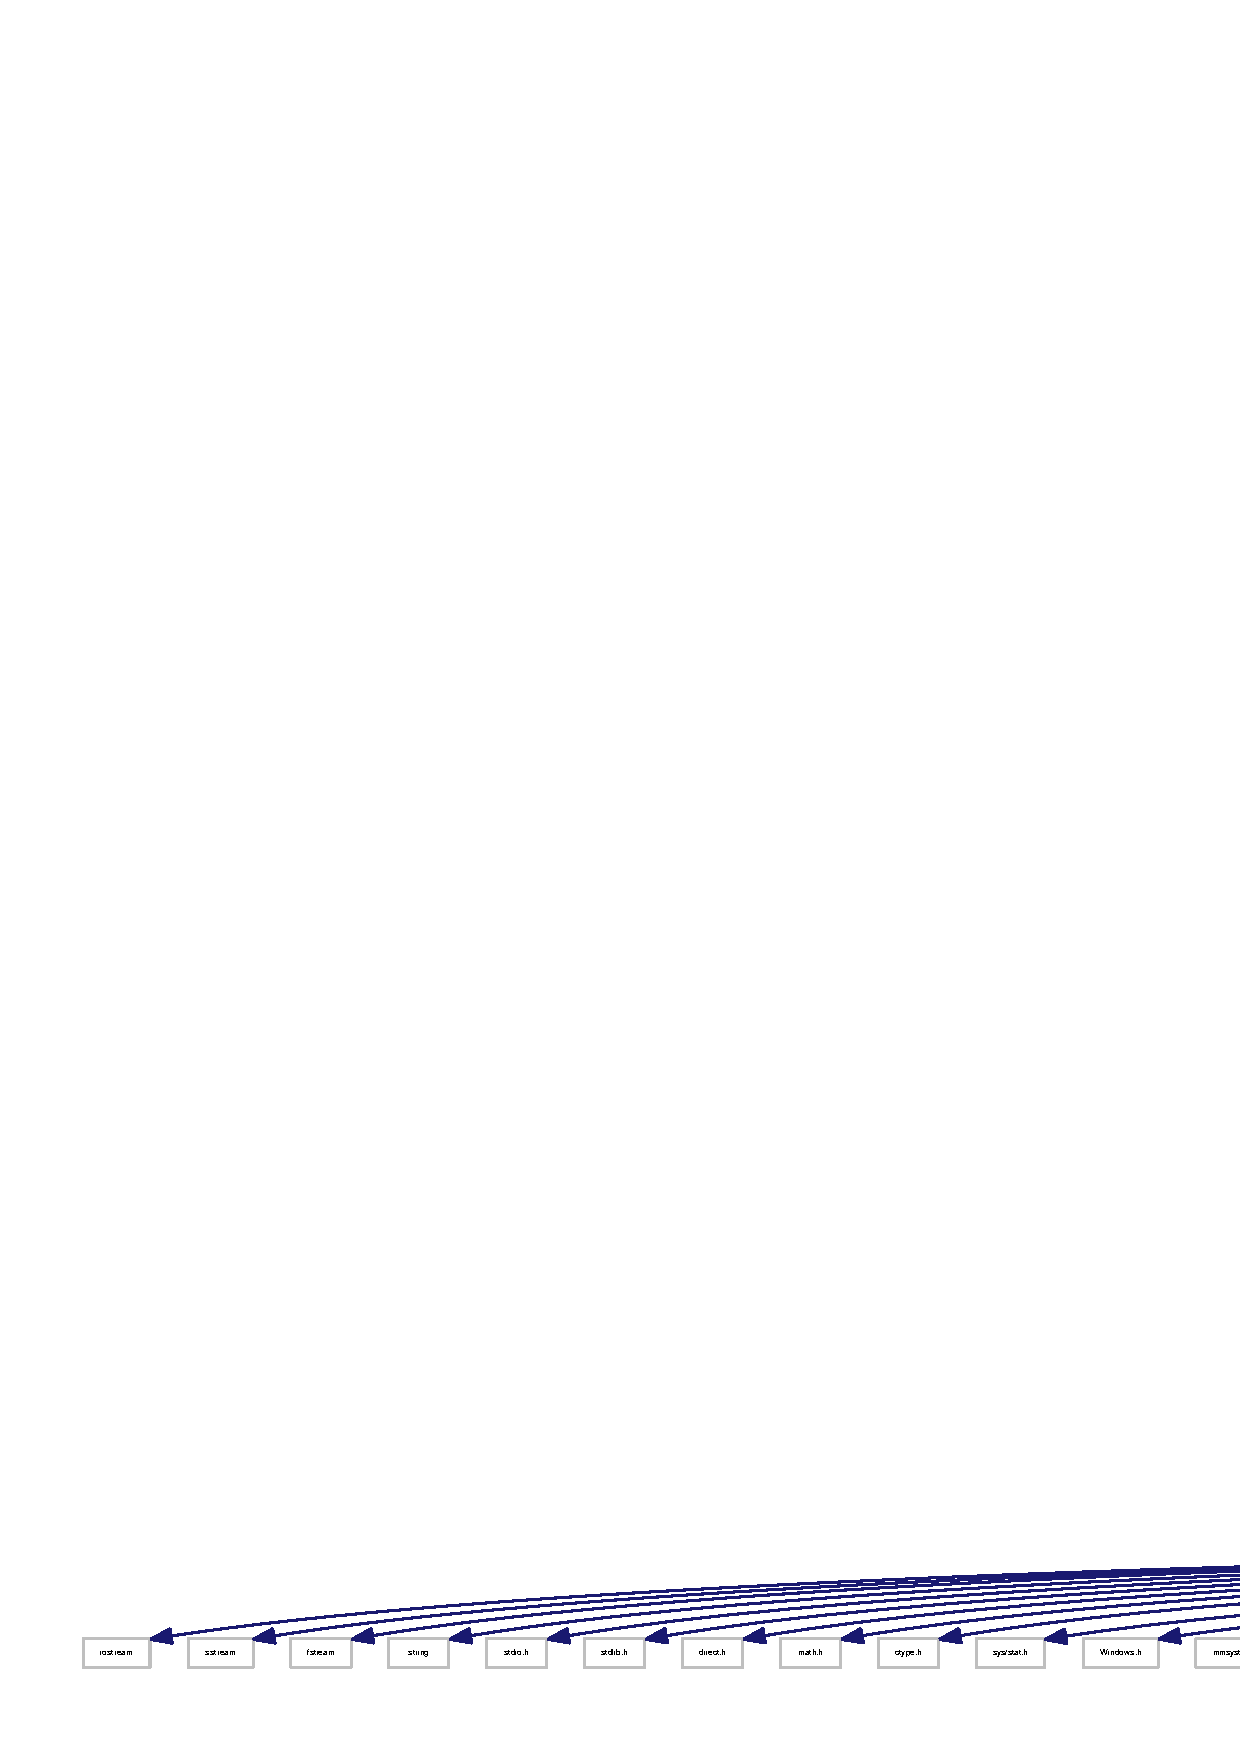
\includegraphics[width=350pt]{stdafx_8h__incl}
\end{center}
\end{figure}
\subsection*{マクロ定義}
\begin{DoxyCompactItemize}
\item 
\#define {\bf \-\_\-\-C\-R\-T\-\_\-\-S\-E\-C\-U\-R\-E\-\_\-\-N\-O\-\_\-\-W\-A\-R\-N\-I\-N\-G\-S}
\item 
\#define {\bf W\-I\-D\-T\-H}~640
\begin{DoxyCompactList}\small\item\em $<$名前空間 \end{DoxyCompactList}\item 
\#define {\bf H\-E\-I\-G\-H\-T}~480
\begin{DoxyCompactList}\small\item\em 画像の高さ \end{DoxyCompactList}\item 
\#define {\bf A\-L\-L\-P\-I\-X\-E\-L}~{\bf W\-I\-D\-T\-H}$\ast${\bf H\-E\-I\-G\-H\-T}
\begin{DoxyCompactList}\small\item\em 1フレームの全ピクセル数 \end{DoxyCompactList}\item 
\#define {\bf N\-O\-C}~128
\begin{DoxyCompactList}\small\item\em Number of Characters.(ファイルの名前を付けるときの文字数制限) \end{DoxyCompactList}\end{DoxyCompactItemize}


\subsection{詳解}
標準のシステム,インクルードファイル,または参照回数が多く,かつあまり変更されない,プロジェクト専用のインクルードファイルを記述する. \begin{DoxyDate}{日付}
2015.\-11.\-22 
\end{DoxyDate}
\begin{DoxyAuthor}{著者}
H.\-Shigehara 
\end{DoxyAuthor}


 {\bf stdafx.\-h} に定義があります。



\subsection{マクロ定義詳解}
\index{stdafx.\-h@{stdafx.\-h}!\-\_\-\-C\-R\-T\-\_\-\-S\-E\-C\-U\-R\-E\-\_\-\-N\-O\-\_\-\-W\-A\-R\-N\-I\-N\-G\-S@{\-\_\-\-C\-R\-T\-\_\-\-S\-E\-C\-U\-R\-E\-\_\-\-N\-O\-\_\-\-W\-A\-R\-N\-I\-N\-G\-S}}
\index{\-\_\-\-C\-R\-T\-\_\-\-S\-E\-C\-U\-R\-E\-\_\-\-N\-O\-\_\-\-W\-A\-R\-N\-I\-N\-G\-S@{\-\_\-\-C\-R\-T\-\_\-\-S\-E\-C\-U\-R\-E\-\_\-\-N\-O\-\_\-\-W\-A\-R\-N\-I\-N\-G\-S}!stdafx.h@{stdafx.\-h}}
\subsubsection[{\-\_\-\-C\-R\-T\-\_\-\-S\-E\-C\-U\-R\-E\-\_\-\-N\-O\-\_\-\-W\-A\-R\-N\-I\-N\-G\-S}]{\setlength{\rightskip}{0pt plus 5cm}\#define \-\_\-\-C\-R\-T\-\_\-\-S\-E\-C\-U\-R\-E\-\_\-\-N\-O\-\_\-\-W\-A\-R\-N\-I\-N\-G\-S}\label{stdafx_8h_af08ec37a8c99d747fb60fa15bc28678b}


 stdafx.\-h の 11 行目に定義があります。

\index{stdafx.\-h@{stdafx.\-h}!A\-L\-L\-P\-I\-X\-E\-L@{A\-L\-L\-P\-I\-X\-E\-L}}
\index{A\-L\-L\-P\-I\-X\-E\-L@{A\-L\-L\-P\-I\-X\-E\-L}!stdafx.h@{stdafx.\-h}}
\subsubsection[{A\-L\-L\-P\-I\-X\-E\-L}]{\setlength{\rightskip}{0pt plus 5cm}\#define A\-L\-L\-P\-I\-X\-E\-L~{\bf W\-I\-D\-T\-H}$\ast${\bf H\-E\-I\-G\-H\-T}}\label{stdafx_8h_ada27e1c35871e9e6118bd9818362f01e}


1フレームの全ピクセル数 



 stdafx.\-h の 80 行目に定義があります。

\index{stdafx.\-h@{stdafx.\-h}!H\-E\-I\-G\-H\-T@{H\-E\-I\-G\-H\-T}}
\index{H\-E\-I\-G\-H\-T@{H\-E\-I\-G\-H\-T}!stdafx.h@{stdafx.\-h}}
\subsubsection[{H\-E\-I\-G\-H\-T}]{\setlength{\rightskip}{0pt plus 5cm}\#define H\-E\-I\-G\-H\-T~480}\label{stdafx_8h_aed89bd71aee8be823e8a20ec4e093c1e}


画像の高さ 



 stdafx.\-h の 79 行目に定義があります。

\index{stdafx.\-h@{stdafx.\-h}!N\-O\-C@{N\-O\-C}}
\index{N\-O\-C@{N\-O\-C}!stdafx.h@{stdafx.\-h}}
\subsubsection[{N\-O\-C}]{\setlength{\rightskip}{0pt plus 5cm}\#define N\-O\-C~128}\label{stdafx_8h_a5d8ba032e2fdf7b2561f508164124f3e}


Number of Characters.(ファイルの名前を付けるときの文字数制限) 



 stdafx.\-h の 81 行目に定義があります。



参照元 Drawing\-::gnuplot\-Script\-E\-V3(), Drawing\-::gnuplot\-Script\-E\-V3\-Route(), Drawing\-::gnuplot\-Script\-Time2\-V(), Drawing\-::gnuplot\-Script\-Time2\-Yaw(), main(), System\-::make\-Directory(), System\-::make\-Directory\-Based\-Date(), System\-::open\-Directory(), E\-V3\-Control\-::output6\-Do\-F(), E\-V3\-Control\-::output6\-Do\-F\-Continuous(), E\-V3\-Control\-::output\-Control\-Information(), E\-V3\-Control\-::output\-E\-V3\-Route\-Continuous(), Image\-Processing\-::output\-Image\-Select\-Directory(), Point\-Cloud\-Library\-::output\-Point\-Cloud(), Point\-Cloud\-Library\-::output\-Point\-Cloud\-P\-L\-Y(), System\-::output\-Video(), System\-::remove\-Directory() (計17項目).

\index{stdafx.\-h@{stdafx.\-h}!W\-I\-D\-T\-H@{W\-I\-D\-T\-H}}
\index{W\-I\-D\-T\-H@{W\-I\-D\-T\-H}!stdafx.h@{stdafx.\-h}}
\subsubsection[{W\-I\-D\-T\-H}]{\setlength{\rightskip}{0pt plus 5cm}\#define W\-I\-D\-T\-H~640}\label{stdafx_8h_a241aeeb764887ae5e3de58b98f04b16d}


$<$名前空間 

画像の幅 

 stdafx.\-h の 78 行目に定義があります。


\section{System.\-cpp ファイル}
\label{_system_8cpp}\index{System.\-cpp@{System.\-cpp}}
{\ttfamily \#include \char`\"{}Path\-Tracking\-And\-Induction\-Of\-The\-Robot.\-hpp\char`\"{}}\\*
{\ttfamily \#include \char`\"{}System.\-hpp\char`\"{}}\\*

\section{System.\-hpp ファイル}
\label{_system_8hpp}\index{System.\-hpp@{System.\-hpp}}
{\ttfamily \#include \char`\"{}Path\-Tracking\-And\-Induction\-Of\-The\-Robot.\-hpp\char`\"{}}\\*
System.\-hpp の依存先関係図\-:\nopagebreak
\begin{figure}[H]
\begin{center}
\leavevmode
\includegraphics[width=106pt]{_system_8hpp__incl}
\end{center}
\end{figure}
被依存関係図\-:\nopagebreak
\begin{figure}[H]
\begin{center}
\leavevmode
\includegraphics[width=132pt]{_system_8hpp__dep__incl}
\end{center}
\end{figure}
\subsection*{クラス}
\begin{DoxyCompactItemize}
\item 
class {\bf System}
\begin{DoxyCompactList}\small\item\em システム関連の処理を行うクラス \end{DoxyCompactList}\end{DoxyCompactItemize}

%--- End generated contents ---

% Index
\newpage
\phantomsection
\addcontentsline{toc}{chapter}{索引}
\printindex

\end{document}
